\documentclass[mathserif, aspectratio=169]{beamer}
\usetheme{odenpecos}
\setbeamertemplate{itemize/enumerate body begin}{\fontsize{8.8}{9}\selectfont}
\setbeamertemplate{itemize/enumerate subbody begin}{\fontsize{7.5}{8}\selectfont}
\setbeamertemplate{itemize/enumerate subsubbody begin}{\fontsize{7.5}{8}\selectfont}

% default search path for figures
\graphicspath{{./shared_figures/}{./figures/}}

\newcommand{\zapspace}{\topsep=0pt\partopsep=0pt\itemsep=0pt\parskip=0pt}

\usepackage{multicol}
\usepackage{pict2e}
\usepackage{esdiff}
\usepackage{multimedia}
\usepackage{verbatim}
\usepackage{mhchem}

\usepackage[percent]{overpic}
\usepackage[absolute,overlay]{textpos}

\newcommand{\overbar}[1]{\mkern 1.5mu\overline{\mkern-1.5mu#1\mkern-1.5mu}\mkern 1.5mu}
\newcommand{\pp}[2]{\frac{\partial #1}{\partial #2}}
\newcommand{\dd}[2]{\frac{d #1}{d #2}}
\newcommand{\DD}[2]{\frac{D #1}{D #2}}
\newcommand{\mm}{\mathbf{minmod}}
\def\etal{{\it et al~}}
\newcommand{\be}{\begin{eqnarray}}
\newcommand{\ee}{\end{eqnarray}}
\newcommand{\mbb}[1]{\mathbb{#1}} % math blackboard bold
\newcommand{\mcal}[1]{\mathcal{#1}} % math blackboard bold
\newcommand{\mbf}[1]{\mathbf{#1}} % math bold face (for vectors)
\newcommand{\sbf}[1]{\boldsymbol{#1}} % bold face for symbols
\newcommand{\jump}[1]{\llbracket #1 \rrbracket} % jump operator
\newcommand{\avg}[1]{\langle #1 \rangle} % average operator
\newcommand{\rarrow}{\rightarrow}
\newcommand{\Rarrow}{\Rightarrow}
\newcommand{\LRarrow}{\Leftrightarrow}
\newcommand{\vvvert}{|\kern-1pt|\kern-1pt|}
\newcommand{\enorm}[1]{\vvvert #1 \vvvert}
\newcommand{\nutil}{\tilde{\nu}}
\newcommand{\Var}{\mathrm{Var}}
\newcommand{\Cov}{\mathrm{Cov}}


\definecolor{MyDarkGreen}{rgb}{0,0.45,0.08}
\newcommand{\myred}[1]{{\color{red} #1}}
\newcommand{\myblue}[1]{{\color{blue} #1}}
\newcommand{\mygreen}[1]{{\color{MyDarkGreen} #1}}

\newcommand{\sa}{\nu_{\mathrm{sa}}}
\newcommand{\tep}{\tilde{\epsilon}}
\newcommand{\Ssd}{\mathcal{S}} % source term due to slow derivative
\newcommand{\ud}{\,\mathrm{d}}

\newcommand{\Mach}[1]{\ensuremath{\mbox{Ma}_{#1}}}
\newcommand{\Reynolds}{\ensuremath{\mathit{Re}}}
\newcommand{\DensityRat}{\ensuremath{\mathit{DR}}}
\newcommand{\BlowRat}{\ensuremath{\mbox{BR}}}
\newcommand{\VelRat}{\ensuremath{\mathit{VR}}}
\newcommand{\Tau}{\ensuremath{\mathrm{T}}}

\newcommand{\wall}     {\ensuremath{\mathrm{w}}}   % wall subindex
\newcommand{\awall}    {\ensuremath{\mathrm{aw}}}  % adiabatic wall subindex

\newcommand{\commentout}[1]{}

\newcommand{\vect}[1]{\boldsymbol{#1}}
\usepackage{mleftright}
\newcommand{\of}[1]{\mleft( #1 \mright)}
\newcommand{\vth}{v_{\textrm{th}}}
\newcommand{\reals}{\mathbb{R}}
\newcommand{\myint}{\int\limits}
\newcommand{\ddt}[1]{\partial_t #1}
\newcommand{\RR}{\mathbb{R}}
\newcommand{\vr}{v}
%\newcommand{\vtheta}{\theta_{\vect{v}}}
%\newcommand{\vphi}{\varphi_{\vect{v}}}
%\newcommand{\vr}{v_{r}}
\newcommand{\vtheta}{v_{\theta}}
\newcommand{\vphi}{v_{\varphi}}
\newcommand{\vomega}{v_{\omega}}
\newcommand{\vrunit}{\hat{\vect{v}}_{r}}
\newcommand{\vthetaunit}{\hat{\vect{v}}_{\theta}}
\newcommand{\vphiunit}{\hat{\vect{v}}_{\varphi}}
\DeclareMathOperator{\variance}{Var}

\begin{document}
% disable nav
\setbeamertemplate{navigation symbols}{}

% ---------------------------------------------------------------
% Oden/Pecos title page

%\hoffset=.16in
%
%\begin{frame}[plain,t]{}
%\makeatletter
%%\vspace*{0.85cm}
%%\vspace*{0.65cm}
%\includegraphics[height=0.9in,trim=50 40 40 0, clip]{PMSc_159_university_formal_horizontal.pdf} \newline
%%\vspace*{0.3cm}
%\begin{columns}[T,onlytextwidth]
%\column{.8\textwidth}
%{\bf \color{burntorange} \fontfamily{bch}\selectfont 
%% -- Set talk title here
%Solving the Boltzmann equation for electron kinetics using Petrov-Galerkin approach
%% --
%}
%\end{columns}
%\vspace*{.15cm}
%\rule{.8\textwidth}{0.6pt} \newline
%
%\vspace*{0.05cm}
%\setstretch{0.65}
%{\fontfamily{phv}\selectfont
%  { \scriptsize
%    % -- define presenter, authors here
%    Milinda Fernando, Daniil Bochkov, Todd Oliver, George Biros\newline
%    % --
%  }
%  {\color{burntorange} \tiny
%    % -- define role, meeting event, location, etc
%    Year-1 Review $\cdot$ August, 2021 $\cdot$ Austin, TX
%    % --
%  }
%}
%
%\vspace*{1cm}
%%\includegraphics[height=0.3in]{figures/pecos_orange1.png}
%\begin{columns}
%\begin{column}{0.8\linewidth}
%\includegraphics[height=0.5in]{oden_pecos_2020_wordmark.png}\\
%{\scriptsize \url{https://pecos.oden.utexas.edu}}
%\end{column}
%
%\begin{column}{0.2\linewidth}
%\includegraphics[height=0.6in]{psaap3-logo.png}
%\end{column}
%\end{columns}
%
%\end{frame}
%\hoffset=0in
% -- end title slide ---------------------------------------------

\begin{frame}{Collision operator with corrected basis}
	\begin{columns}
		\begin{column}{0.5\textwidth}
			Maxwell polynomials
			\small
			\begin{align*}
				\Phi_{klm} (\vect{v}) &= \exp\left(-\left(\frac{v_r}{v_{th}}\right) ^ 2\right)  P_{kl}\of{\frac{v_r}{v_{th}}} Y_{lm}(v_\theta,v_\phi) \\
				\Psi_{pqs} (\vect{v}) &= P_{pq}\of{\frac{v_r}{v_{th}}} Y_{qs}(v_\theta,v_\phi)
			\end{align*}
			\begin{itemize}
				\item Mass matrix is orthonomal.  
			\end{itemize}
		\end{column}
		\begin{column}{0.5\textwidth}
			B-Splines 
			\small
			\begin{align*}
			\Phi_{klm} (\vect{v}) &= \left(\frac{v_r}{v_{th}}\right)^l P_k\of{\frac{v_r}{v_{th}}} Y_{lm}(v_\theta,v_\phi) \\
			\Psi_{pqs} (\vect{v}) &= \left(\frac{v_r}{v_{th}}\right)^q P_p\of{\frac{v_r}{v_{th}}} Y_{qs}(v_\theta,v_\phi)
			\end{align*}
			\begin{itemize}
				\item ill-conditioning of the mass matrix treated with pseudo inverse. 
				\item knots are placed in log scale
				\item pseudo inverse allows placing knots closer to $v=0$
			\end{itemize}
		\end{column}
	\end{columns}
\end{frame}

%\begin{frame}
%\frametitle{Discretized collision kernel with Maxwell (T=3eV) singular values}
%\begin{table}
%	\centering
%	\begin{tabular}{cc}
%		$l_{max}=0$ &  $l_{max}=1$ \\
%		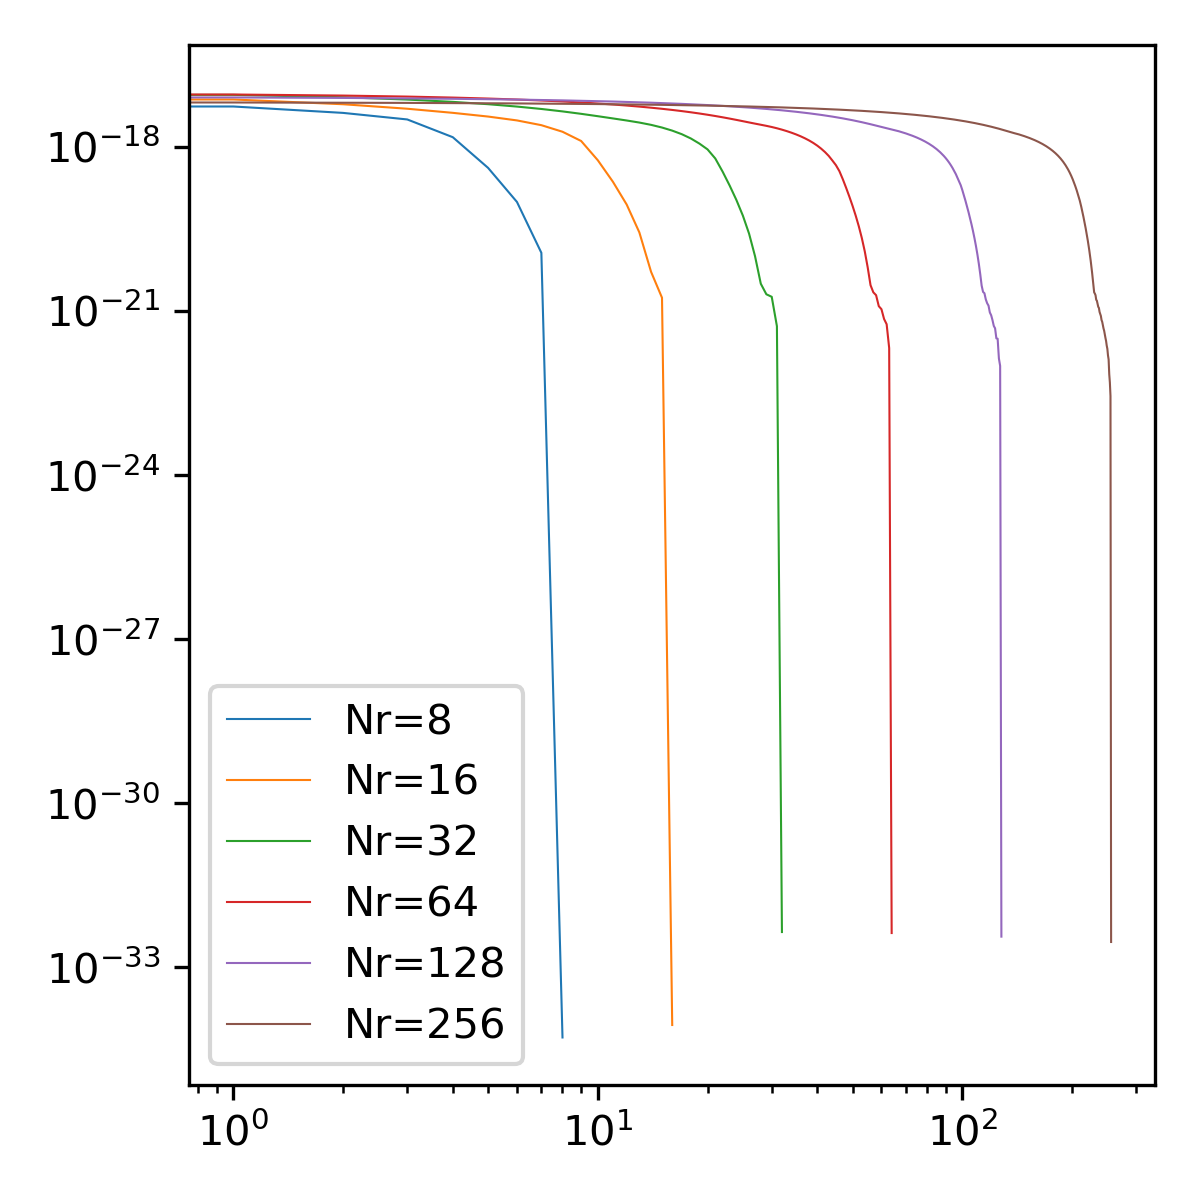
\includegraphics[width=0.3\textwidth]{figures/m_spectrum_3ev_l_max_0.png} & 
%		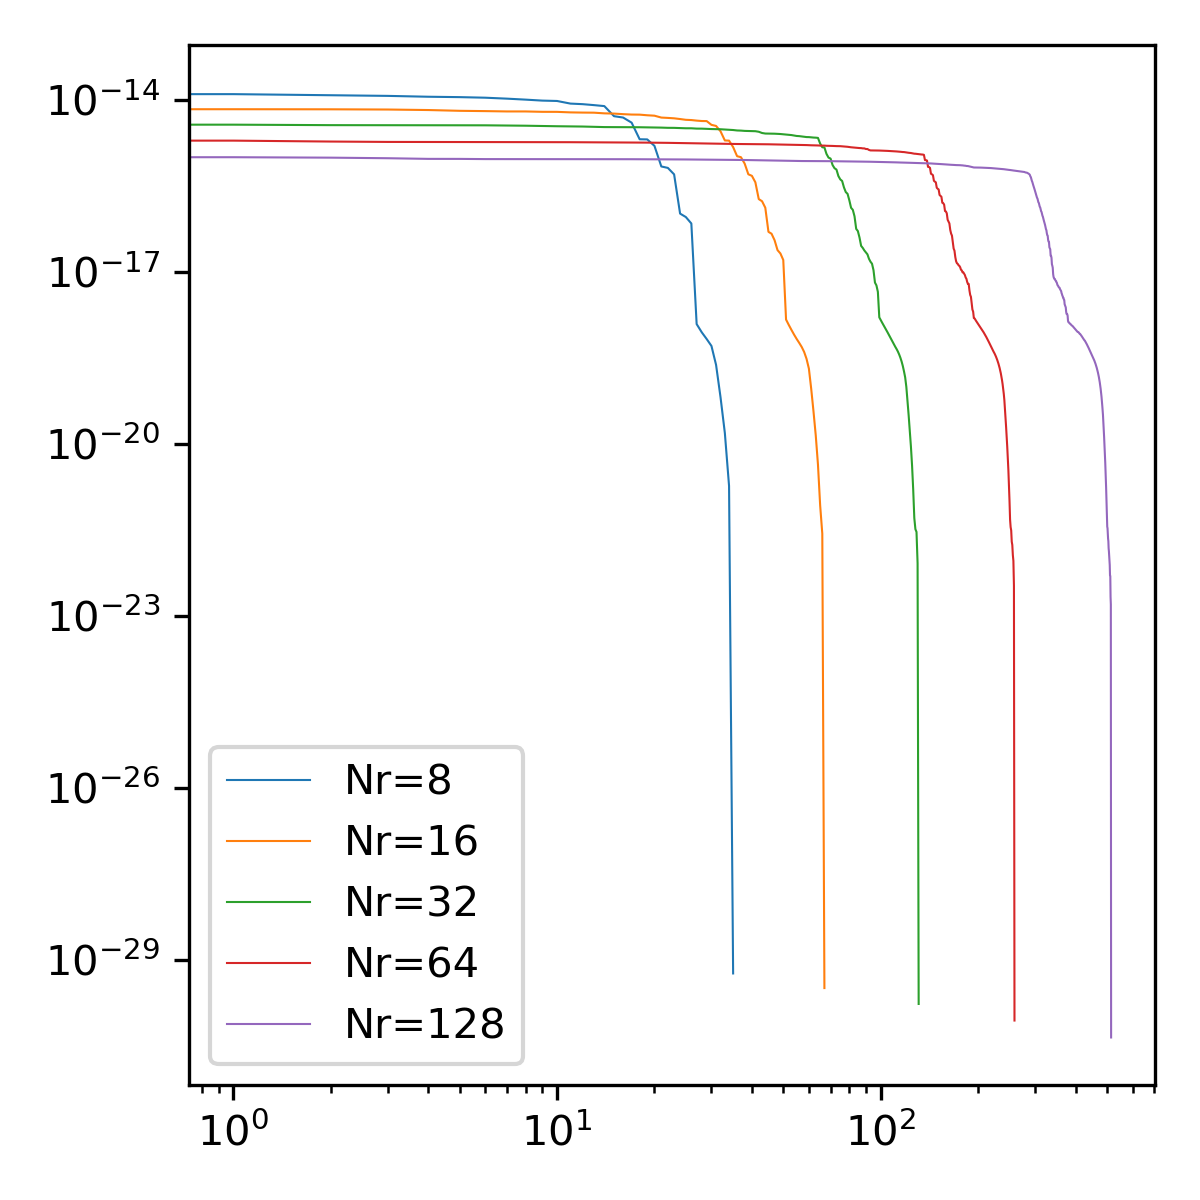
\includegraphics[width=0.3\textwidth]{figures/m_spectrum_3ev_l_max_1.png} 
%	\end{tabular}
%\end{table}
%Currently the differential cross section is uniform across all scattering angles. 
%\end{frame}


\begin{frame}
	\frametitle{Discretized collision kernel (T=3eV) singular values}
	\only<+>{
	\begin{table}
		\centering
		\begin{tabular}{cc}
			Maxwell &  linear splines \\
			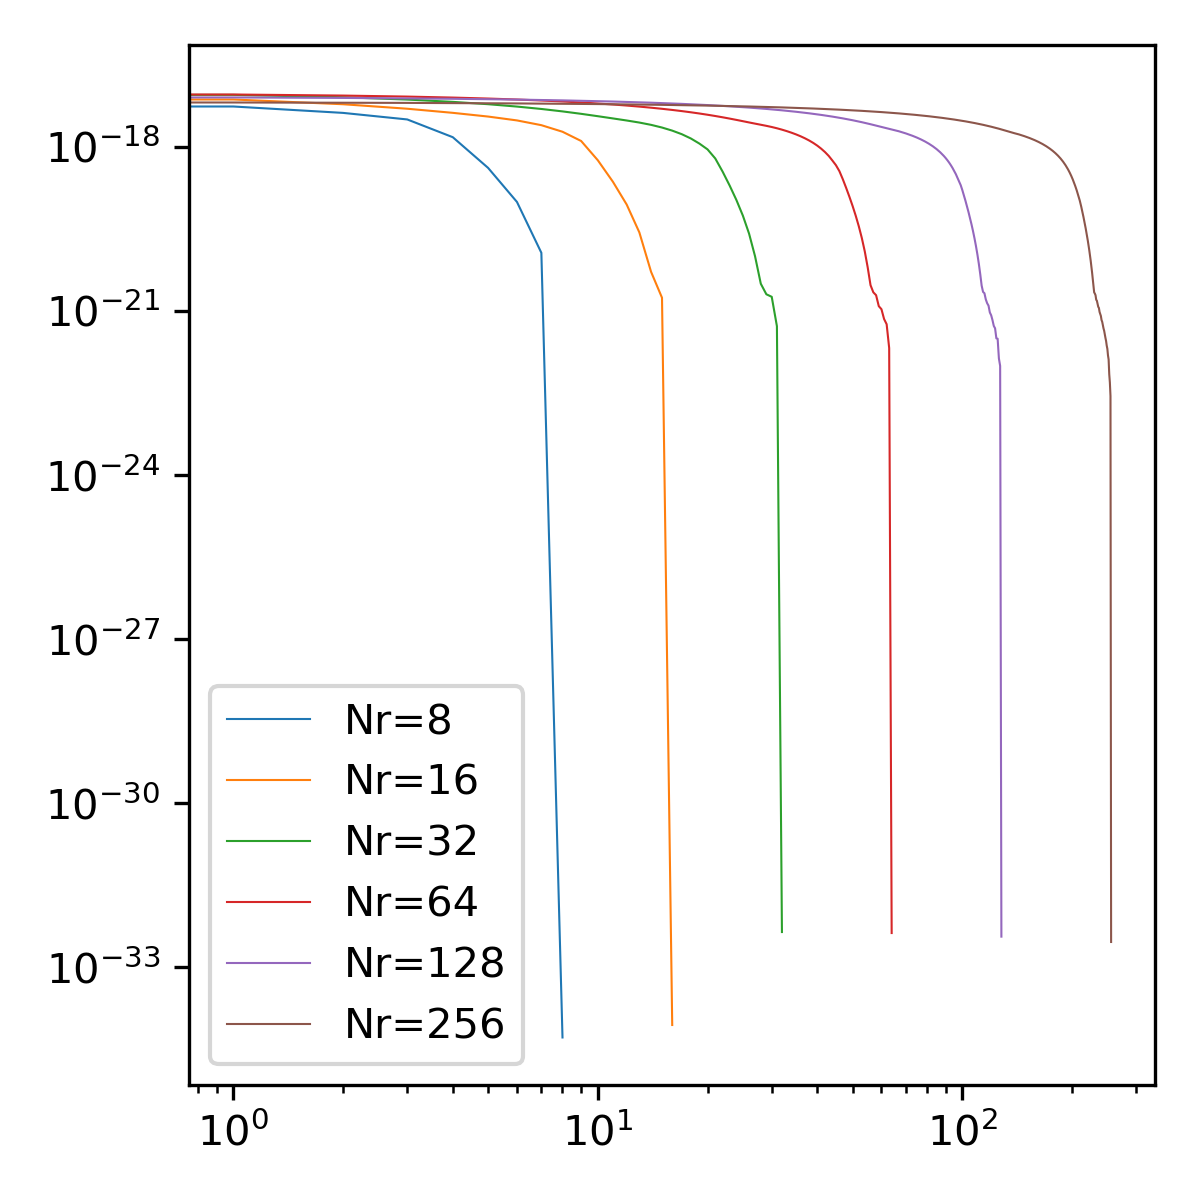
\includegraphics[width=0.35\textwidth]{figures/m_spectrum_3ev_l_max_0.png} & 
			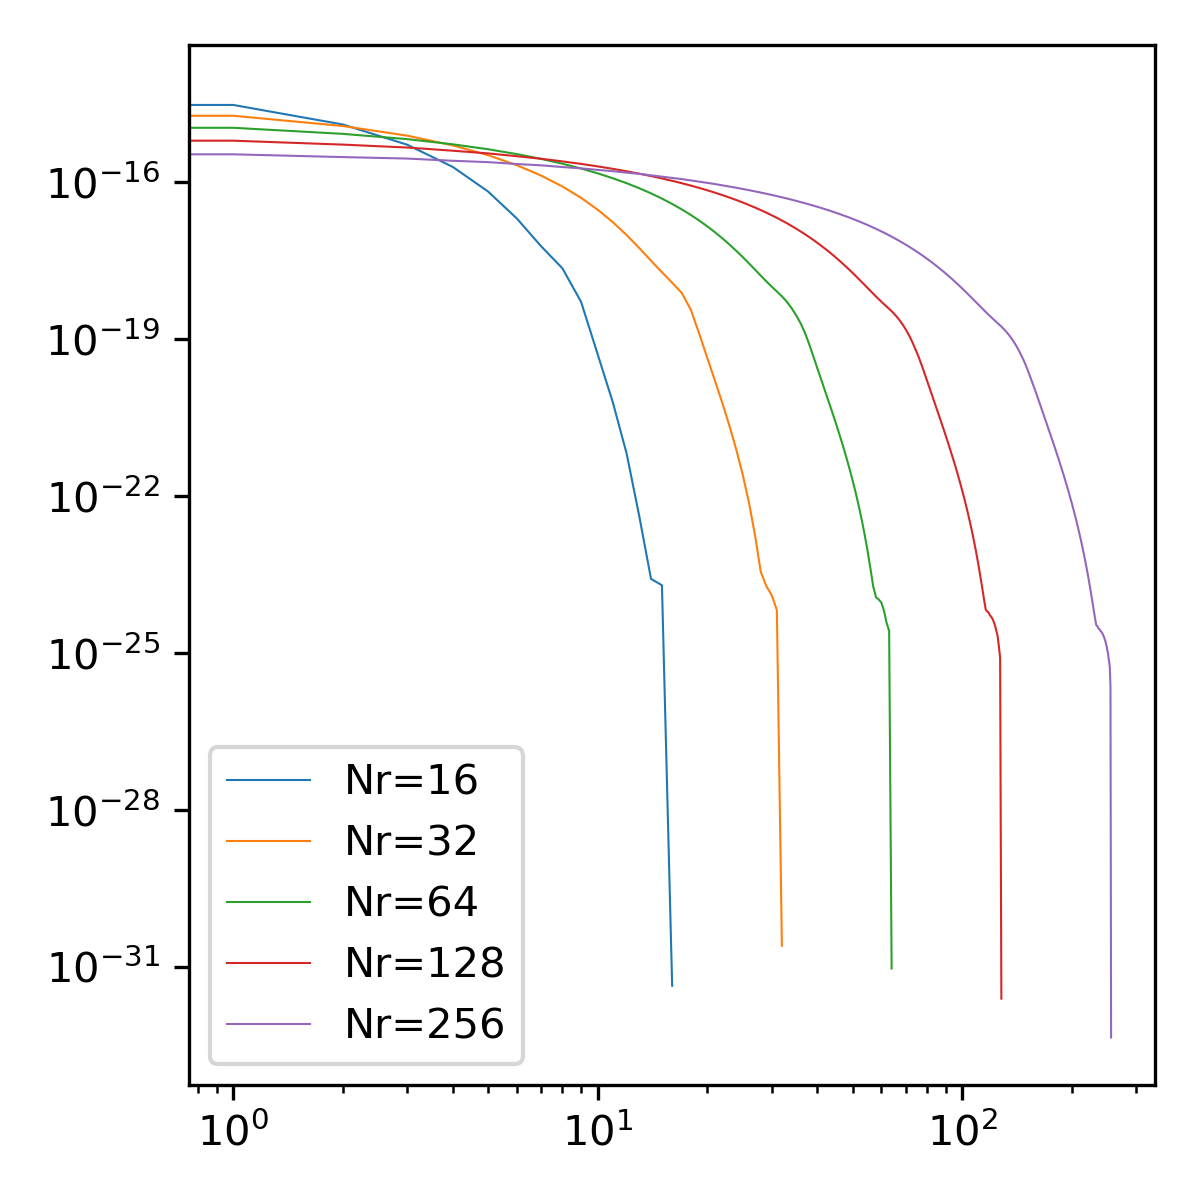
\includegraphics[width=0.35\textwidth]{figures/b_sp1_spectrum_3ev_l_max_0.png} 
		\end{tabular}
	\end{table}}
	\only<+>{
	\begin{table}
		\centering
		\begin{tabular}{cc}
			Maxwell &  quadratic splines \\
			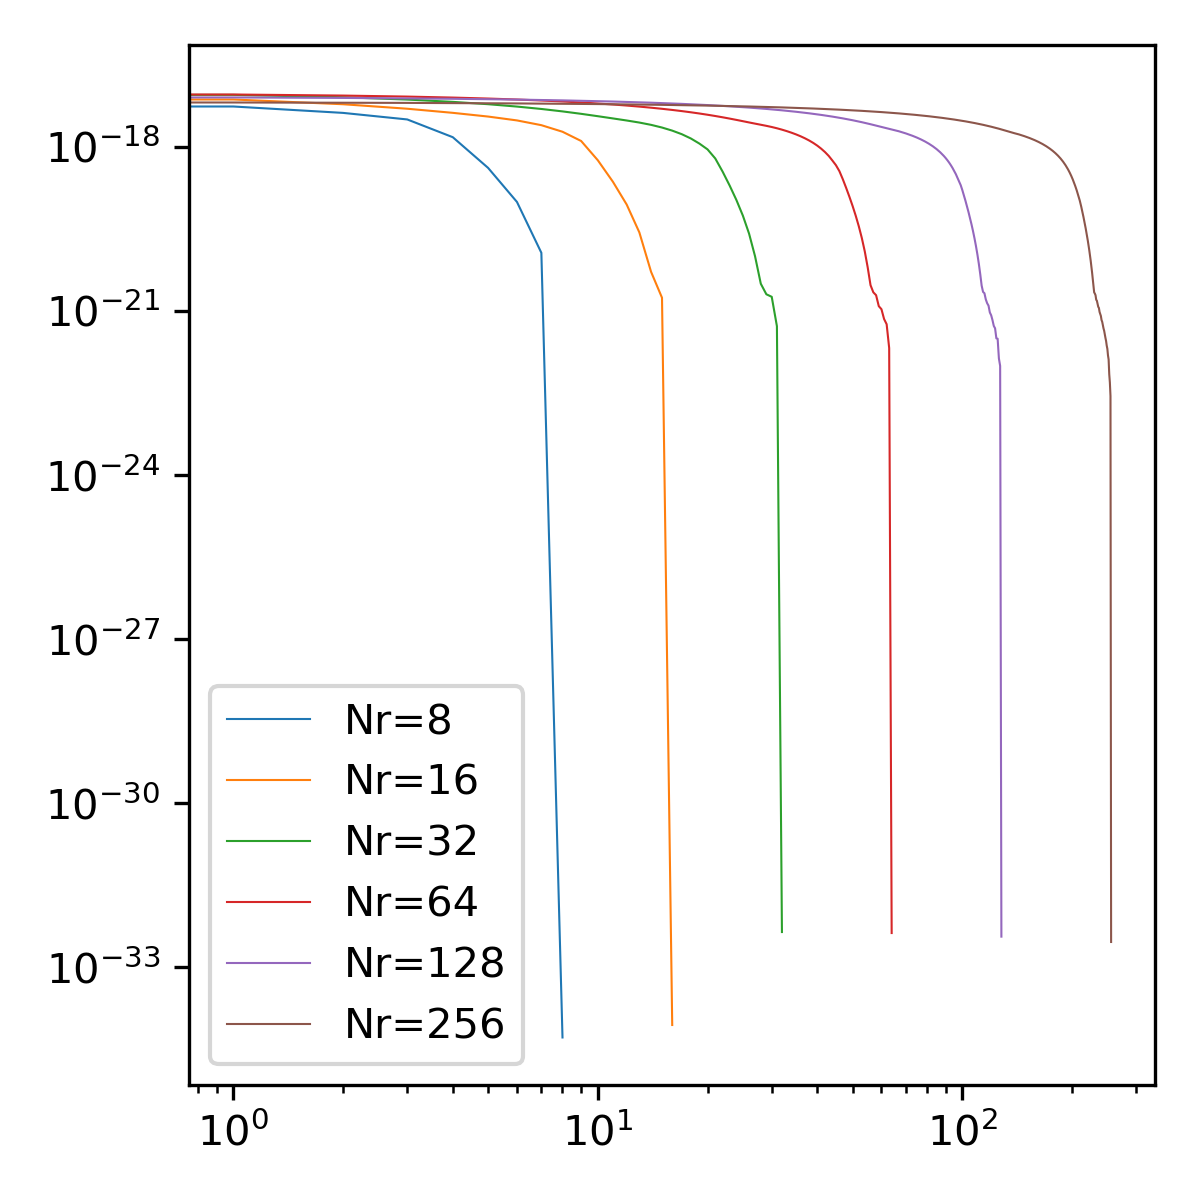
\includegraphics[width=0.35\textwidth]{figures/m_spectrum_3ev_l_max_0.png} & 
			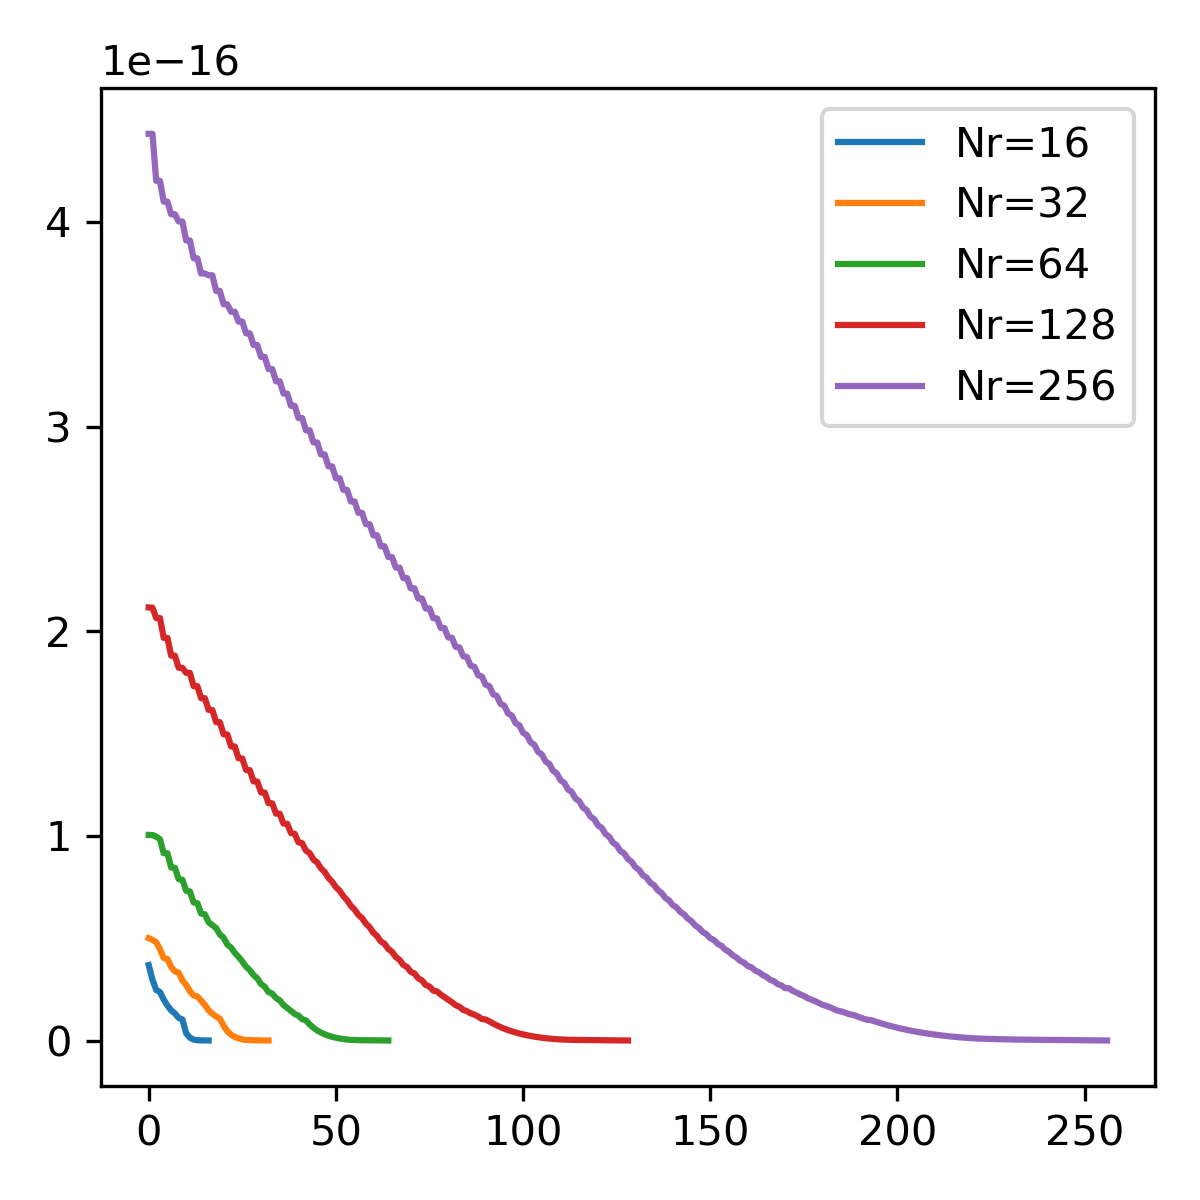
\includegraphics[width=0.35\textwidth]{figures/b_sp2_spectrum_3ev_l_max_0.png} 
		\end{tabular}
\end{table}}
	\only<+>{
	\begin{table}
		\centering
		\begin{tabular}{cc}
			Maxwell &  cubic splines \\
			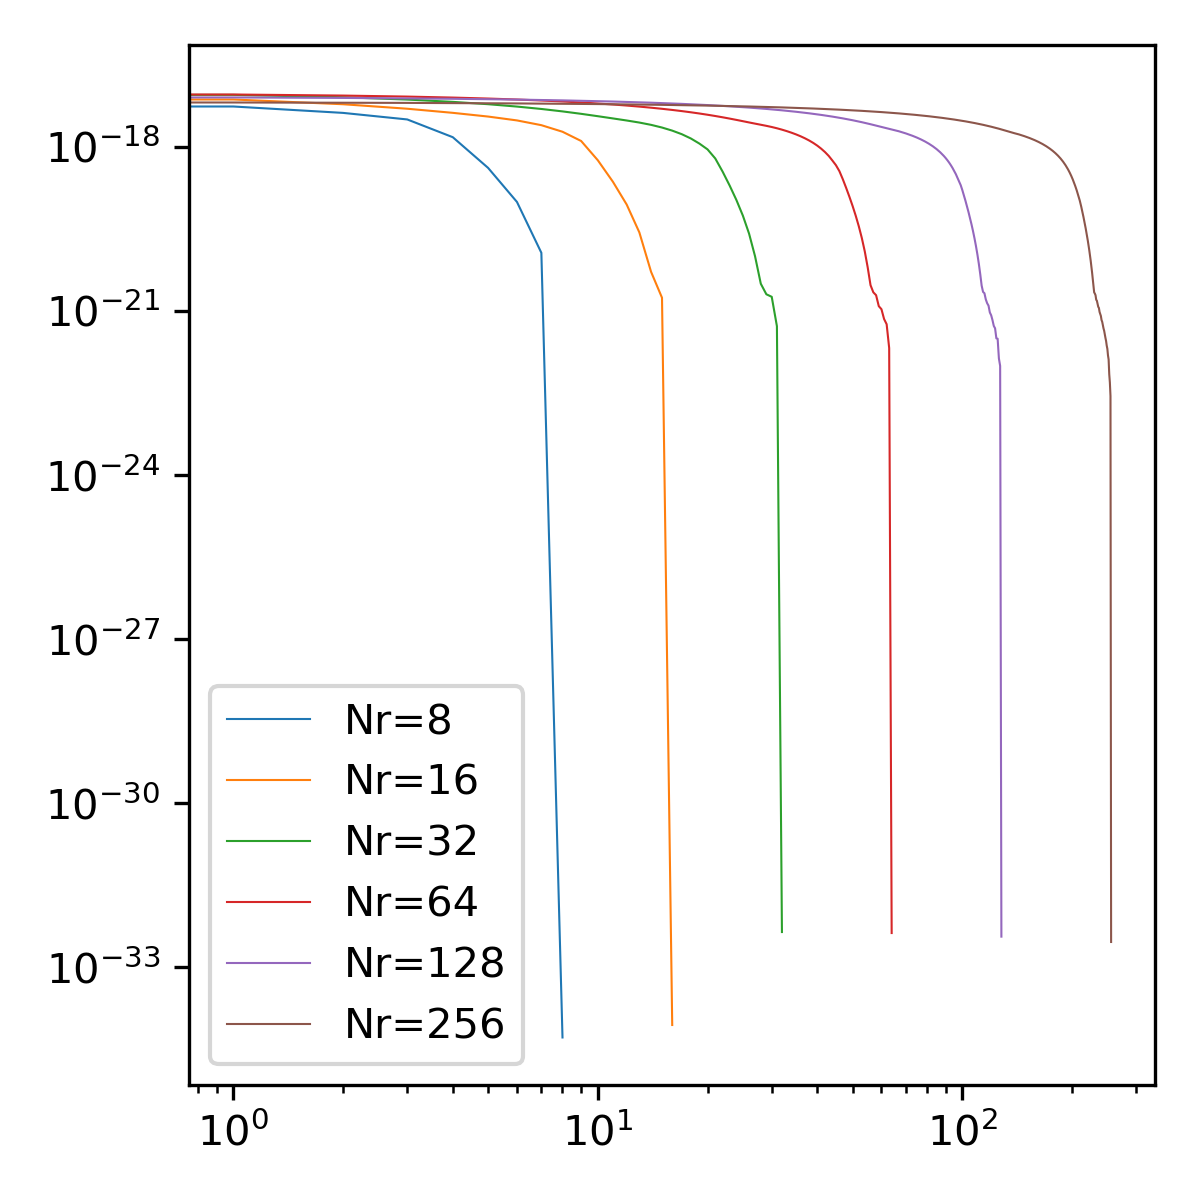
\includegraphics[width=0.35\textwidth]{figures/m_spectrum_3ev_l_max_0.png} & 
			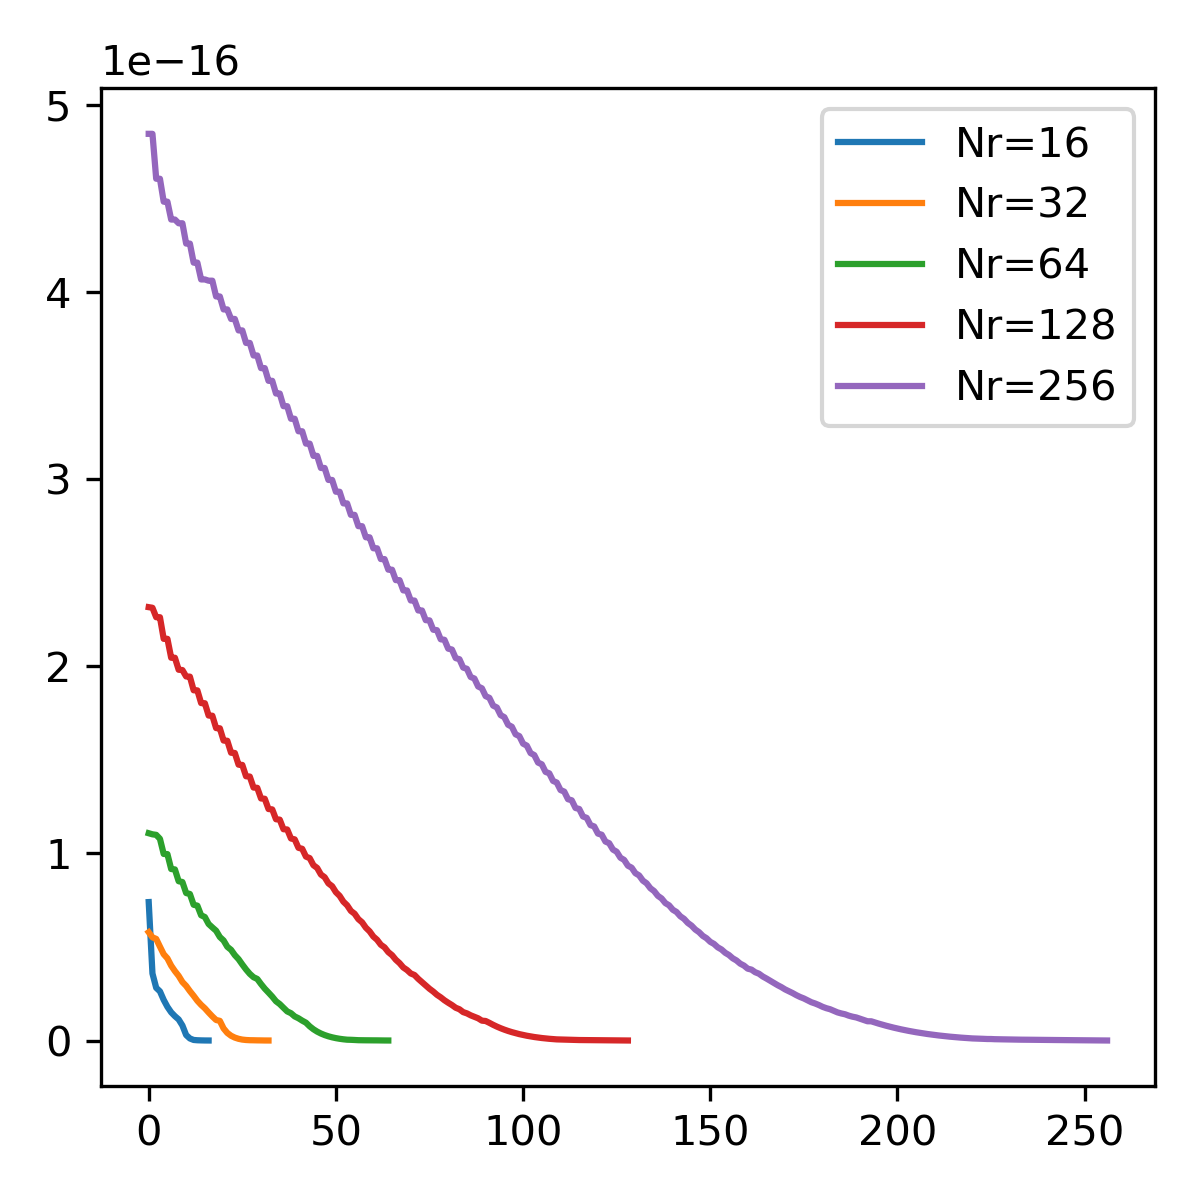
\includegraphics[width=0.35\textwidth]{figures/b_sp3_spectrum_3ev_l_max_0.png} 
		\end{tabular}
\end{table}}
\end{frame}

\begin{frame}
	\frametitle{Elastic collisions (with energy transfer)}
	\only<+>{
		Using Temp(t=0)=1eV, T=1e-6 s
		\begin{table}
			\centering
			\begin{tabular}{cc}
				Maxwell &   quadratic splines\\
				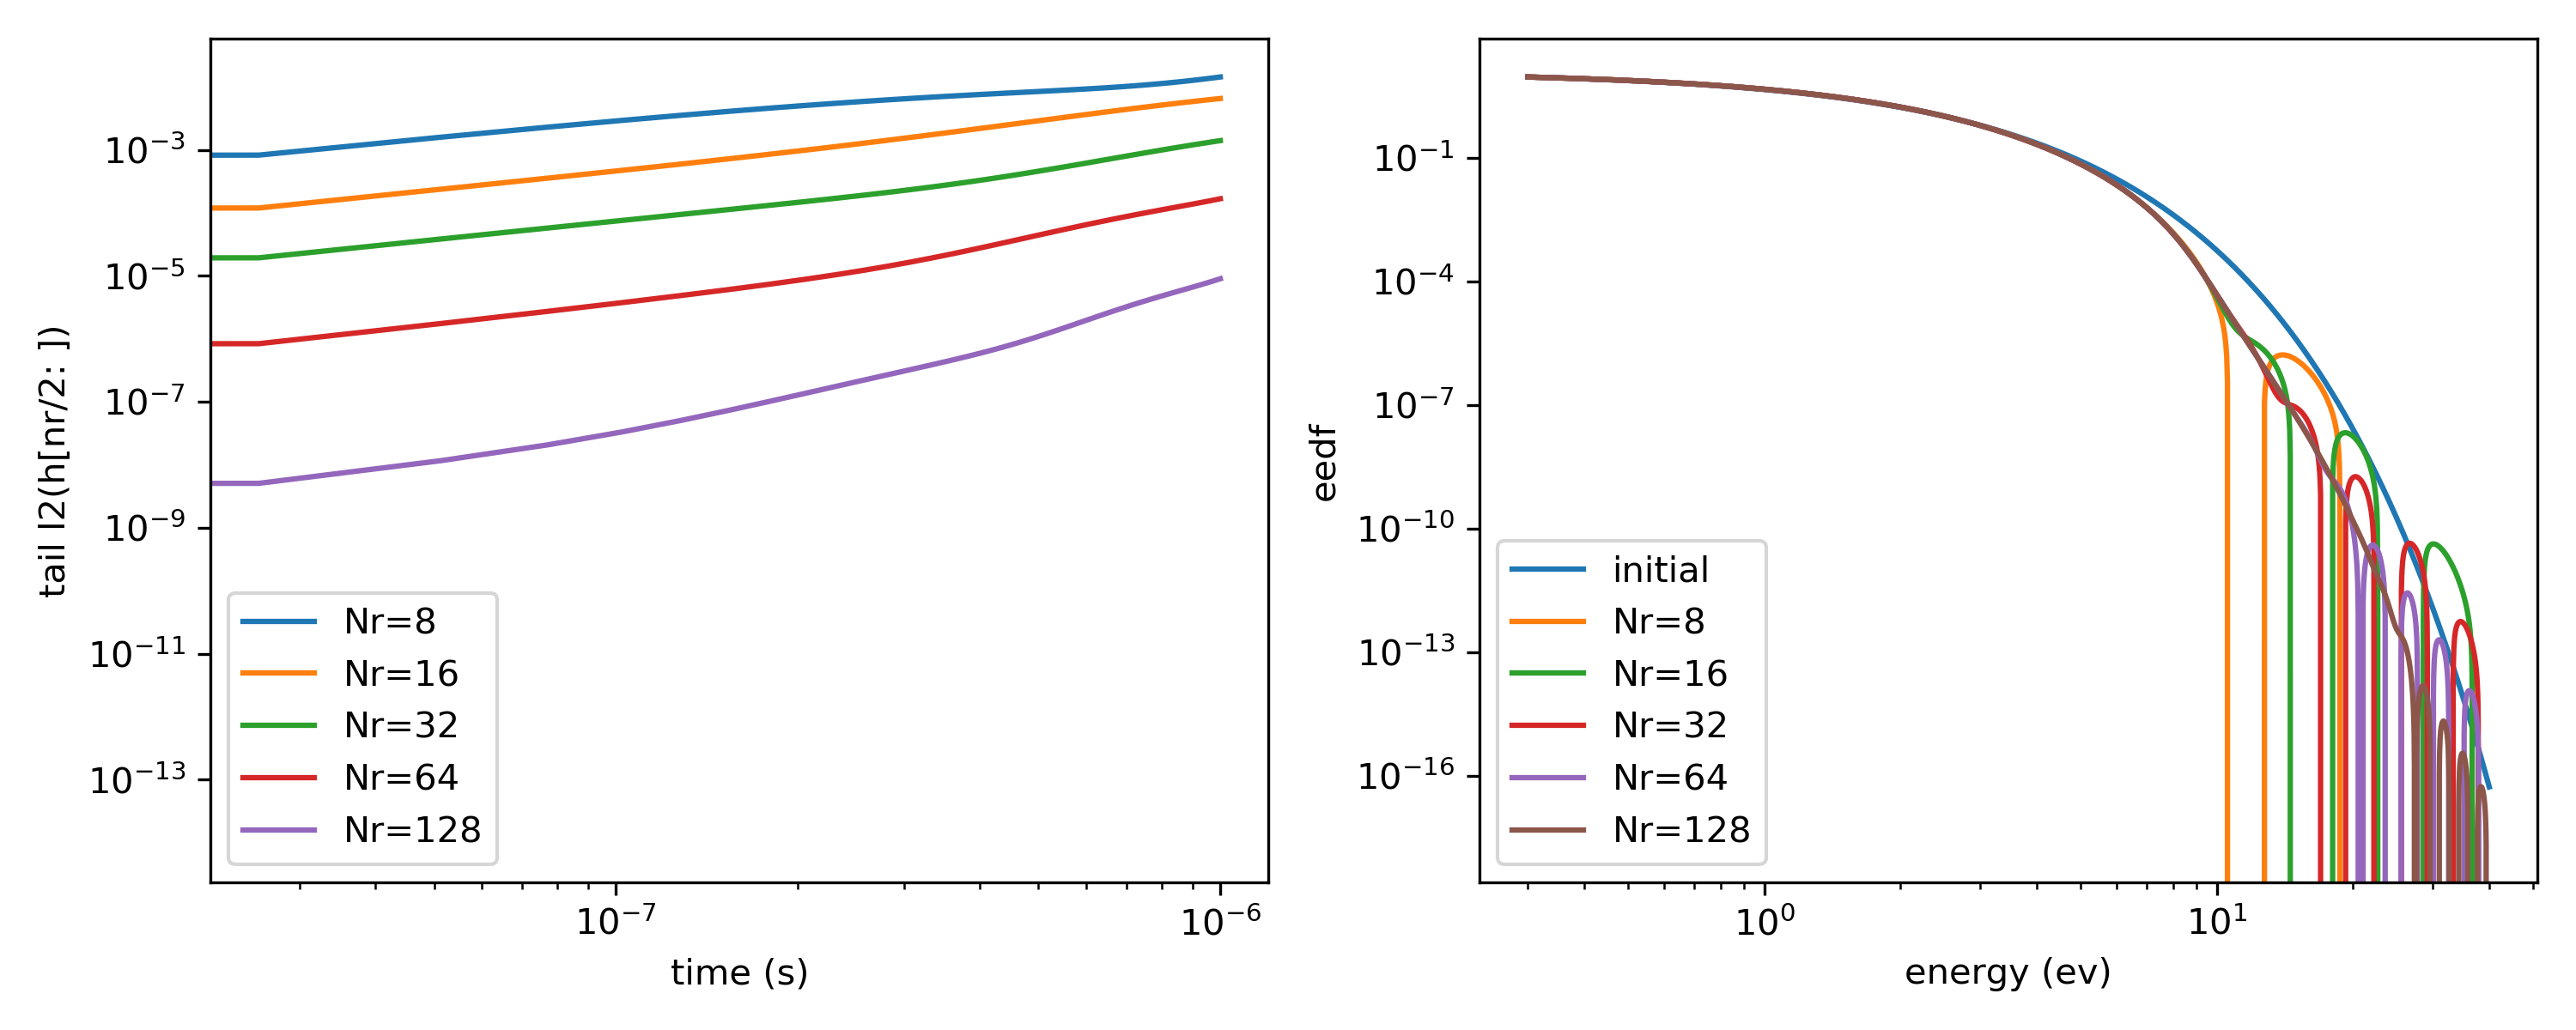
\includegraphics[width=0.48\textwidth]{figures/m_1ev_1e-6.png} & 
				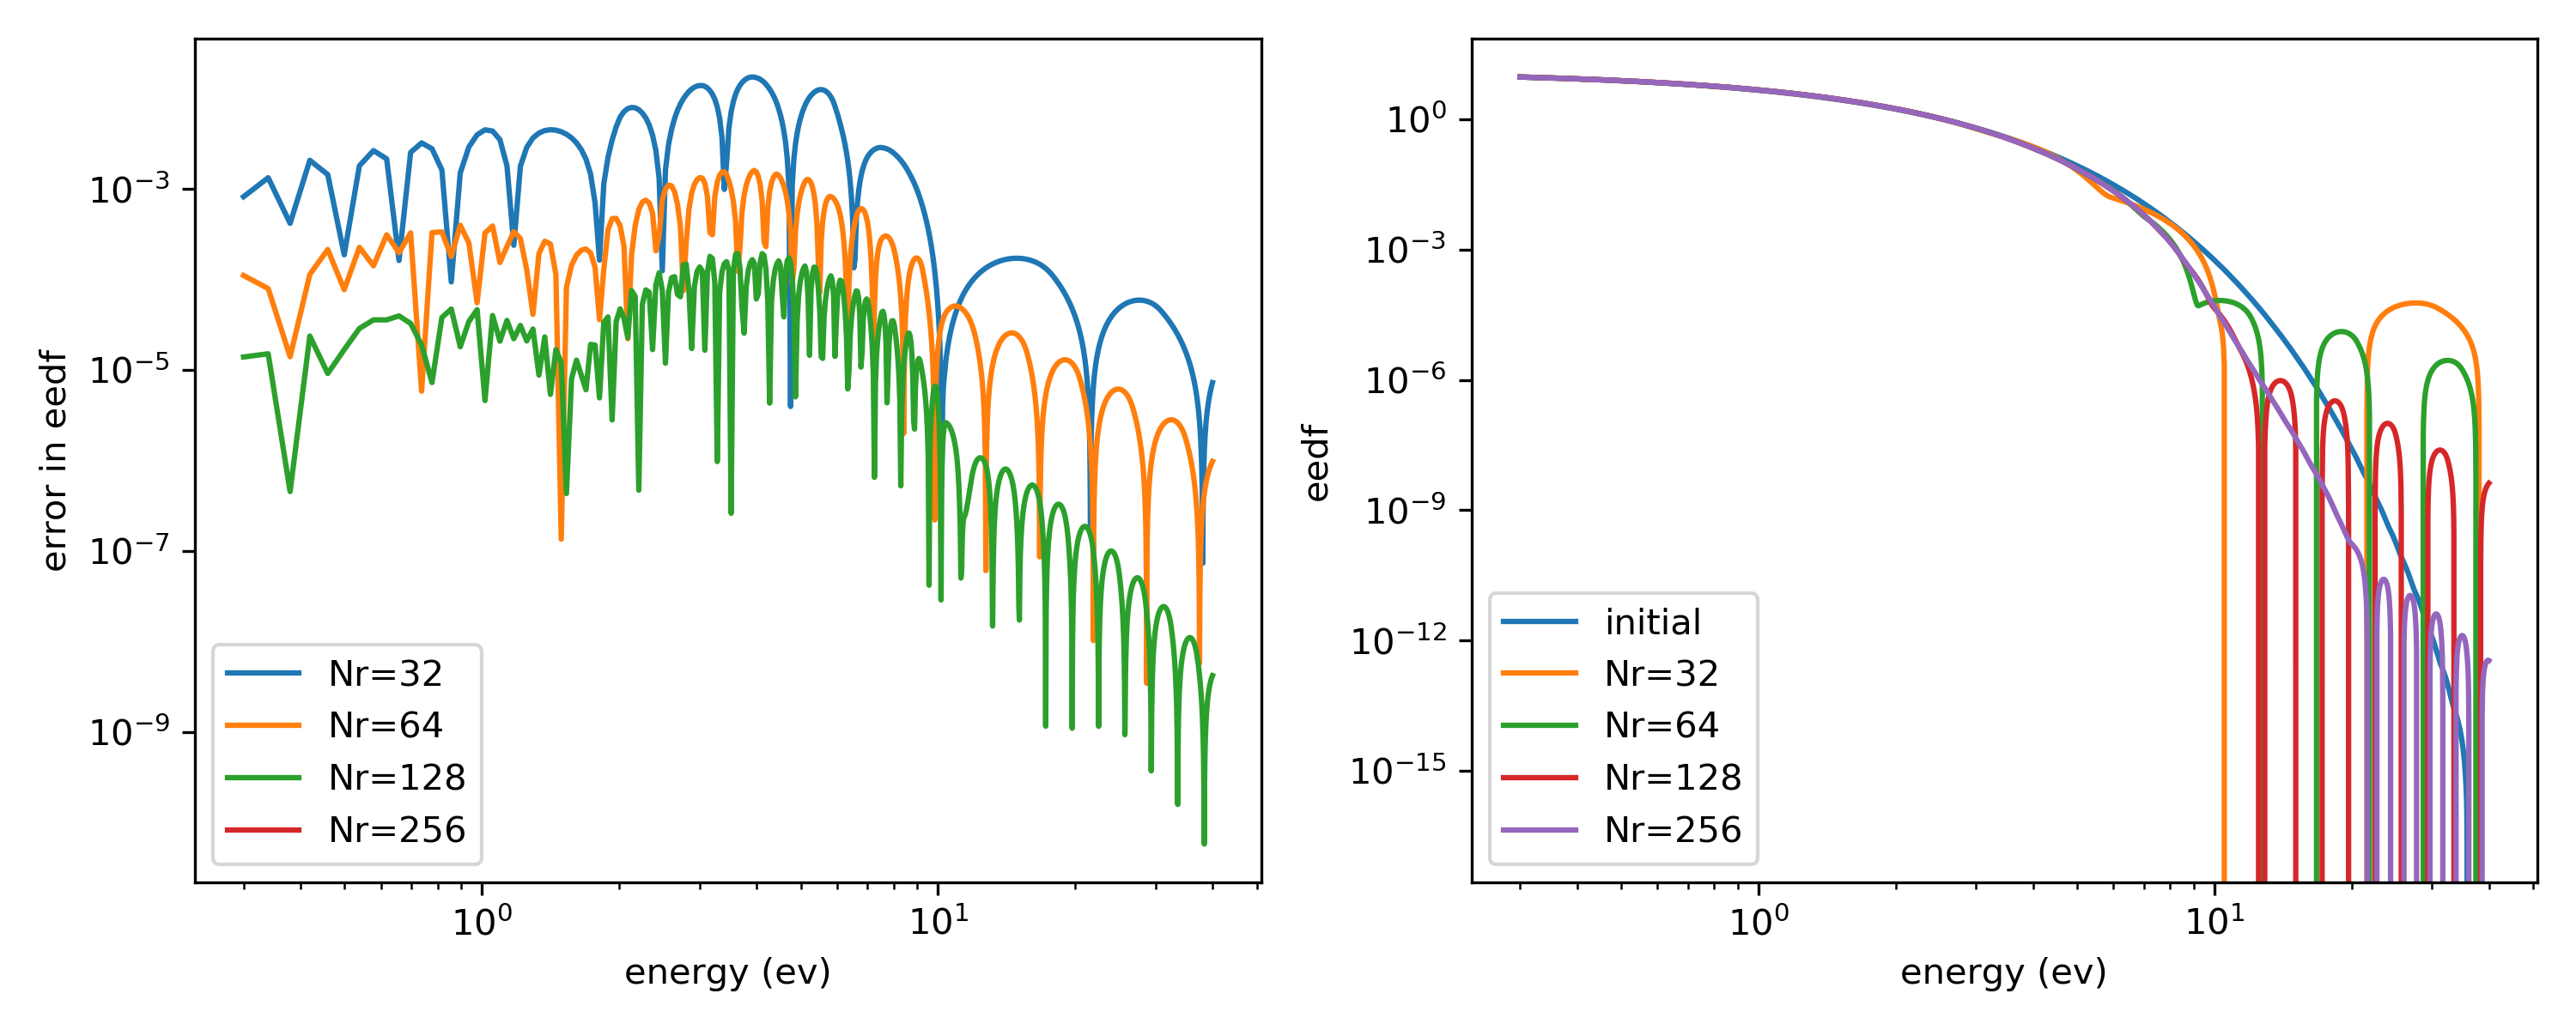
\includegraphics[width=0.48\textwidth]{figures/b_sp2_1ev_1e-6.png} 
			\end{tabular}
	\end{table}
	}
	\only<+>{
	Using Temp(t=0)=3eV, T=1e-6 s
	\begin{table}
		\centering
		\begin{tabular}{cc}
			Maxwell &   quadratic splines\\
			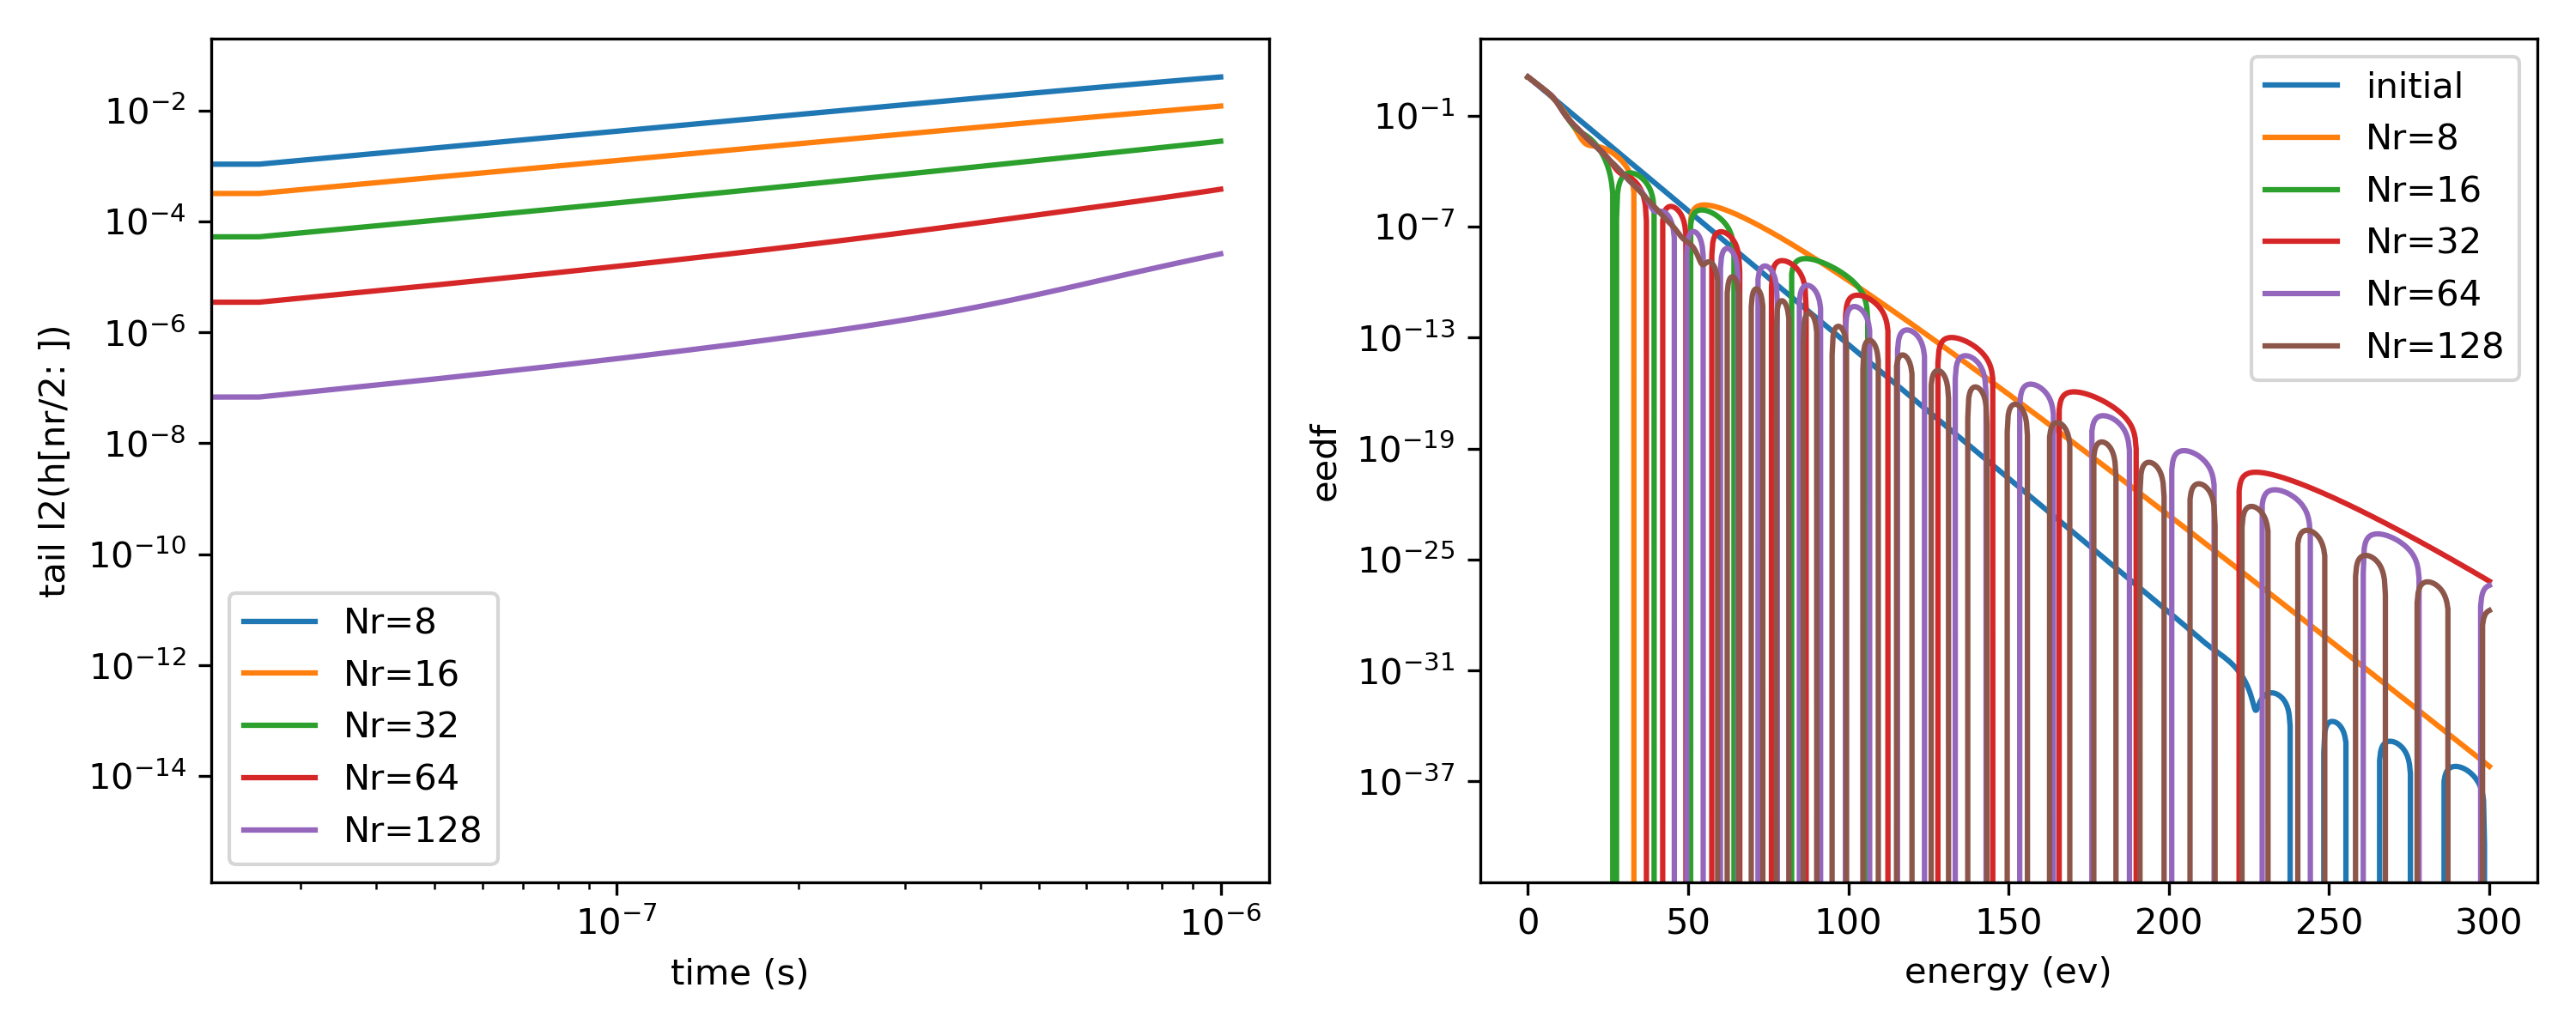
\includegraphics[width=0.48\textwidth]{figures/m_3ev_1e-6.png} & 
			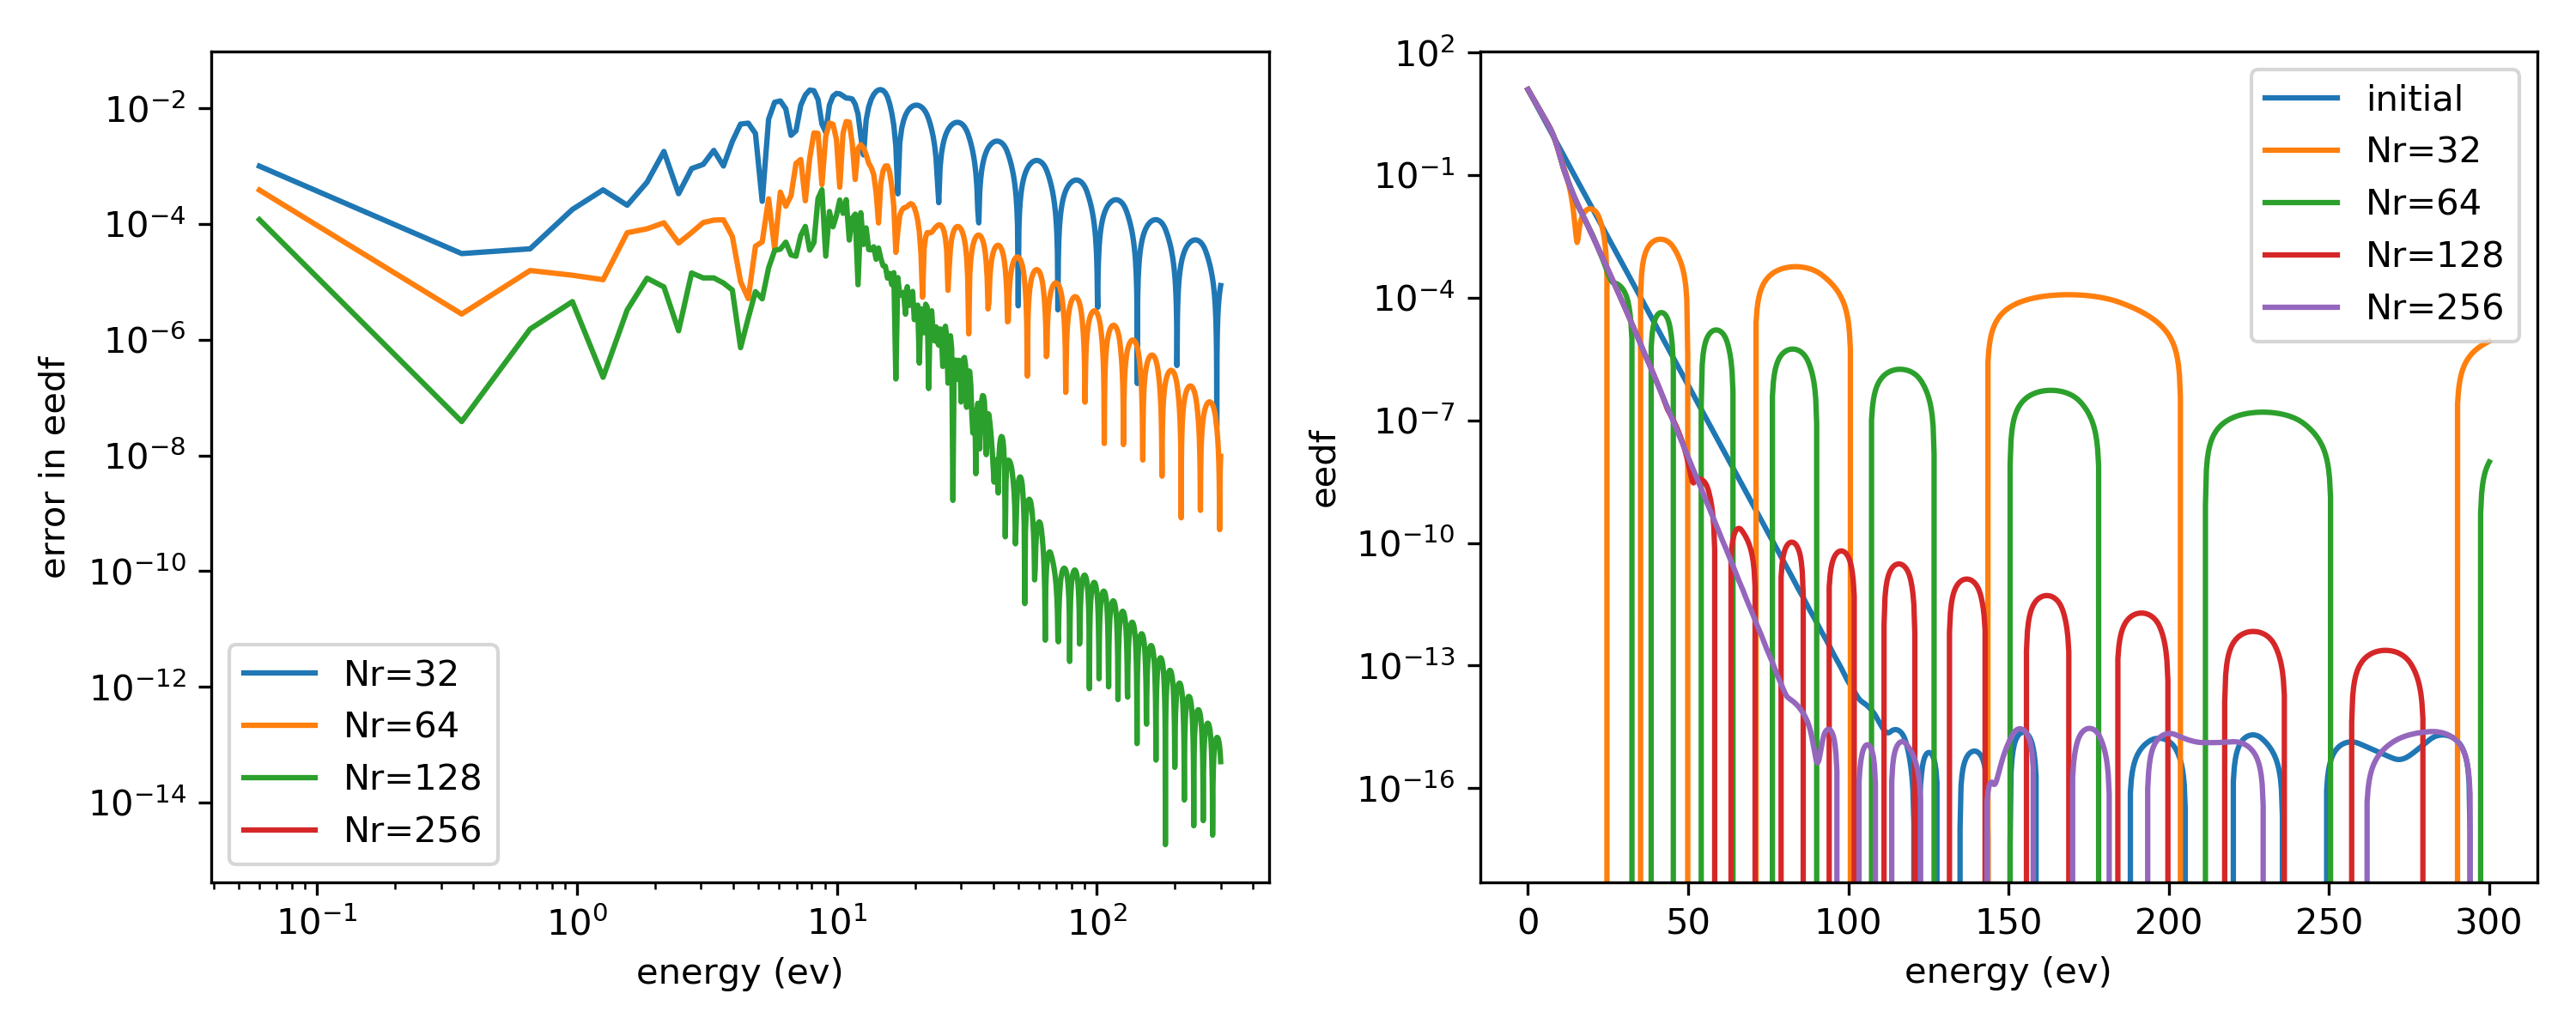
\includegraphics[width=0.48\textwidth]{figures/b_sp2_3ev_1e-6.png} 
		\end{tabular}
	\end{table}
	}

	\only<+>{
	Using Temp(t=0)=5eV, T=1e-6 s
	\begin{table}
		\centering
		\begin{tabular}{cc}
			Maxwell &   quadratic splines\\
			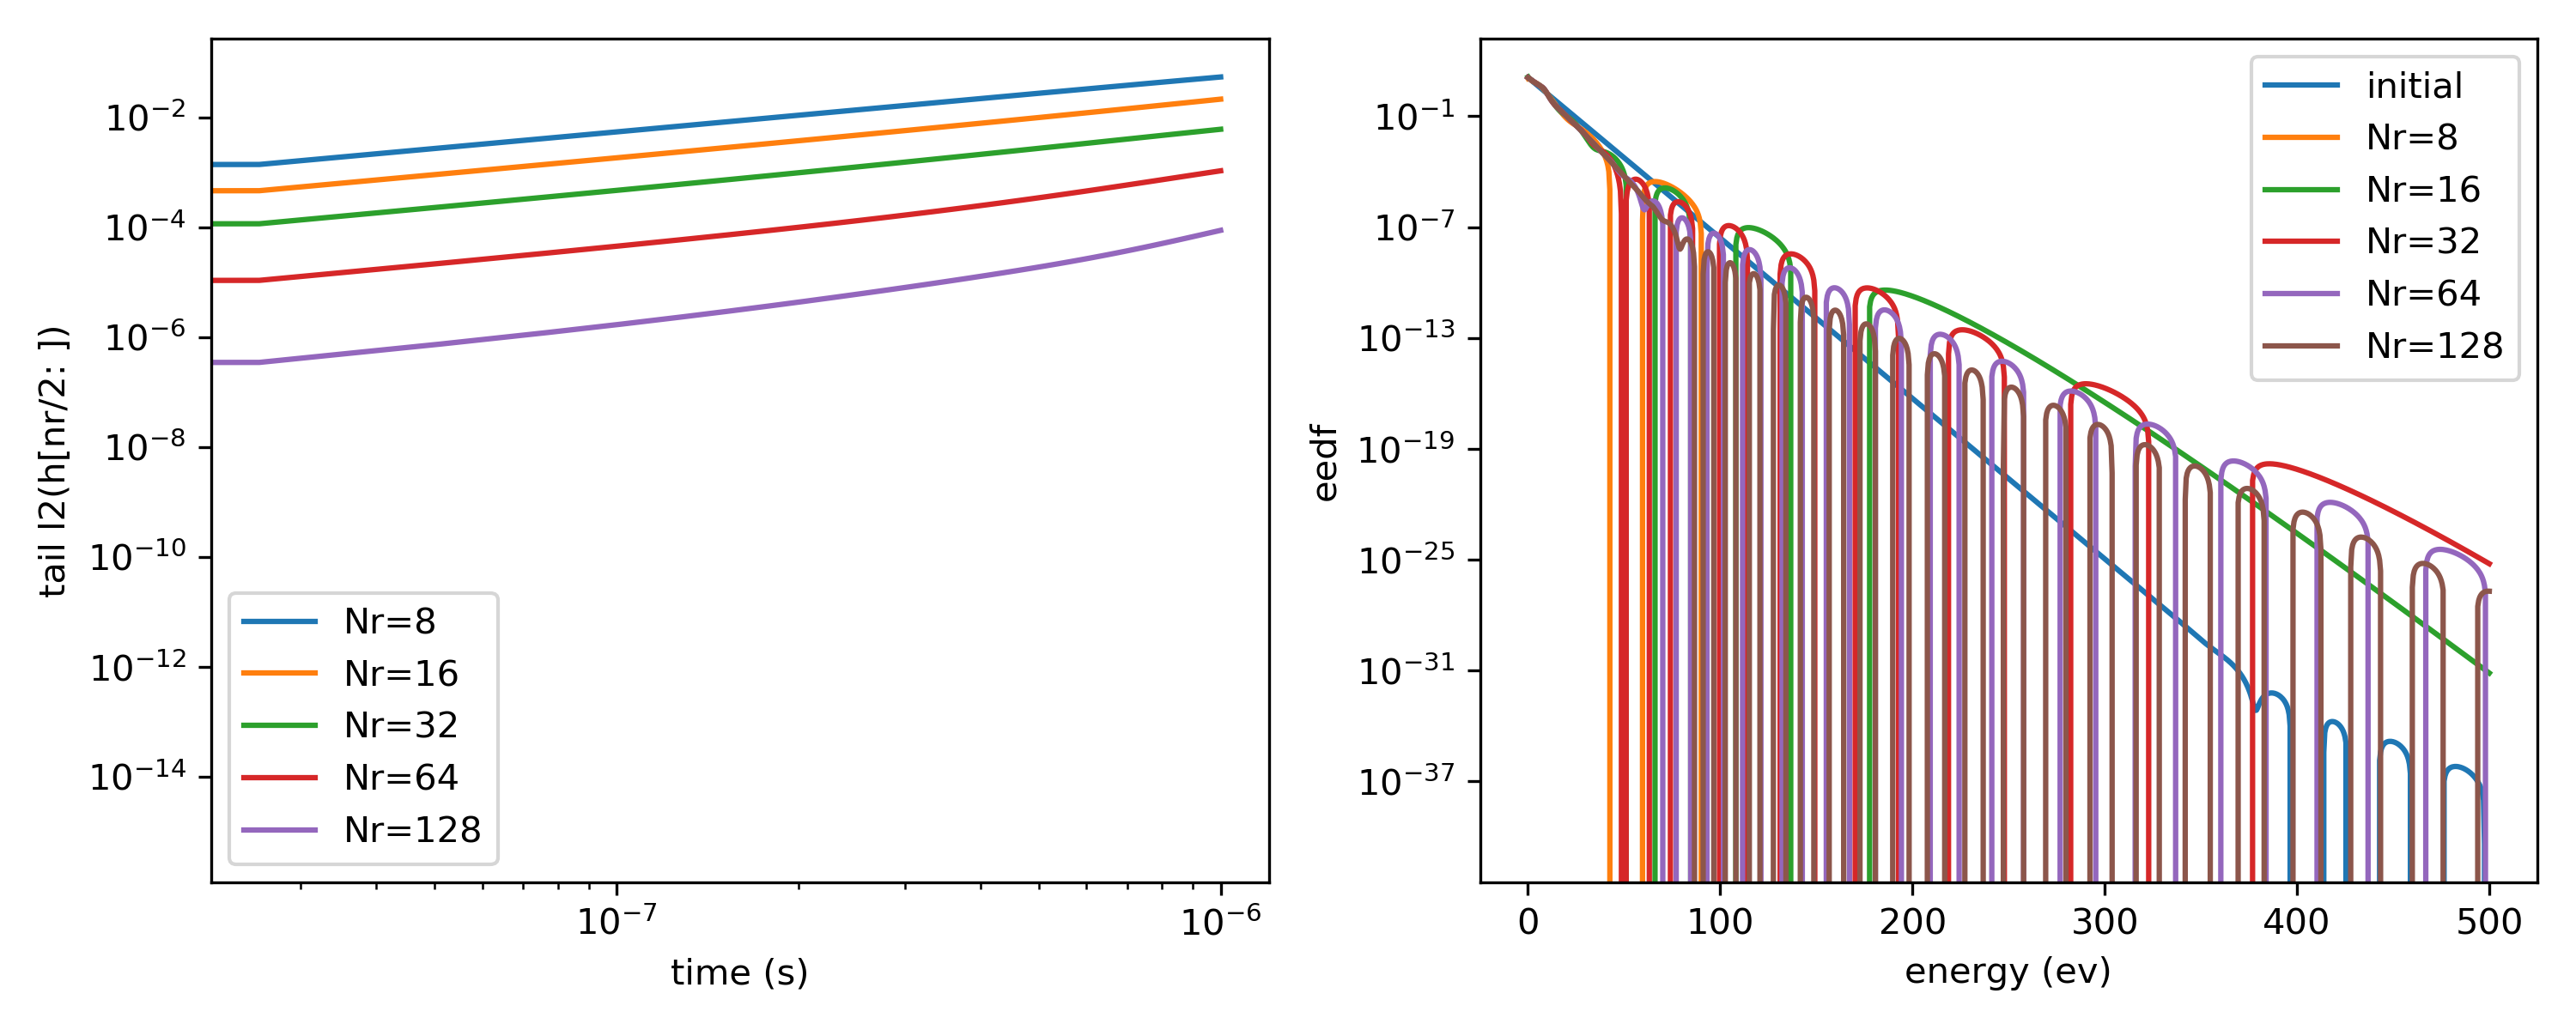
\includegraphics[width=0.48\textwidth]{figures/m_5ev_1e-6.png} & 
			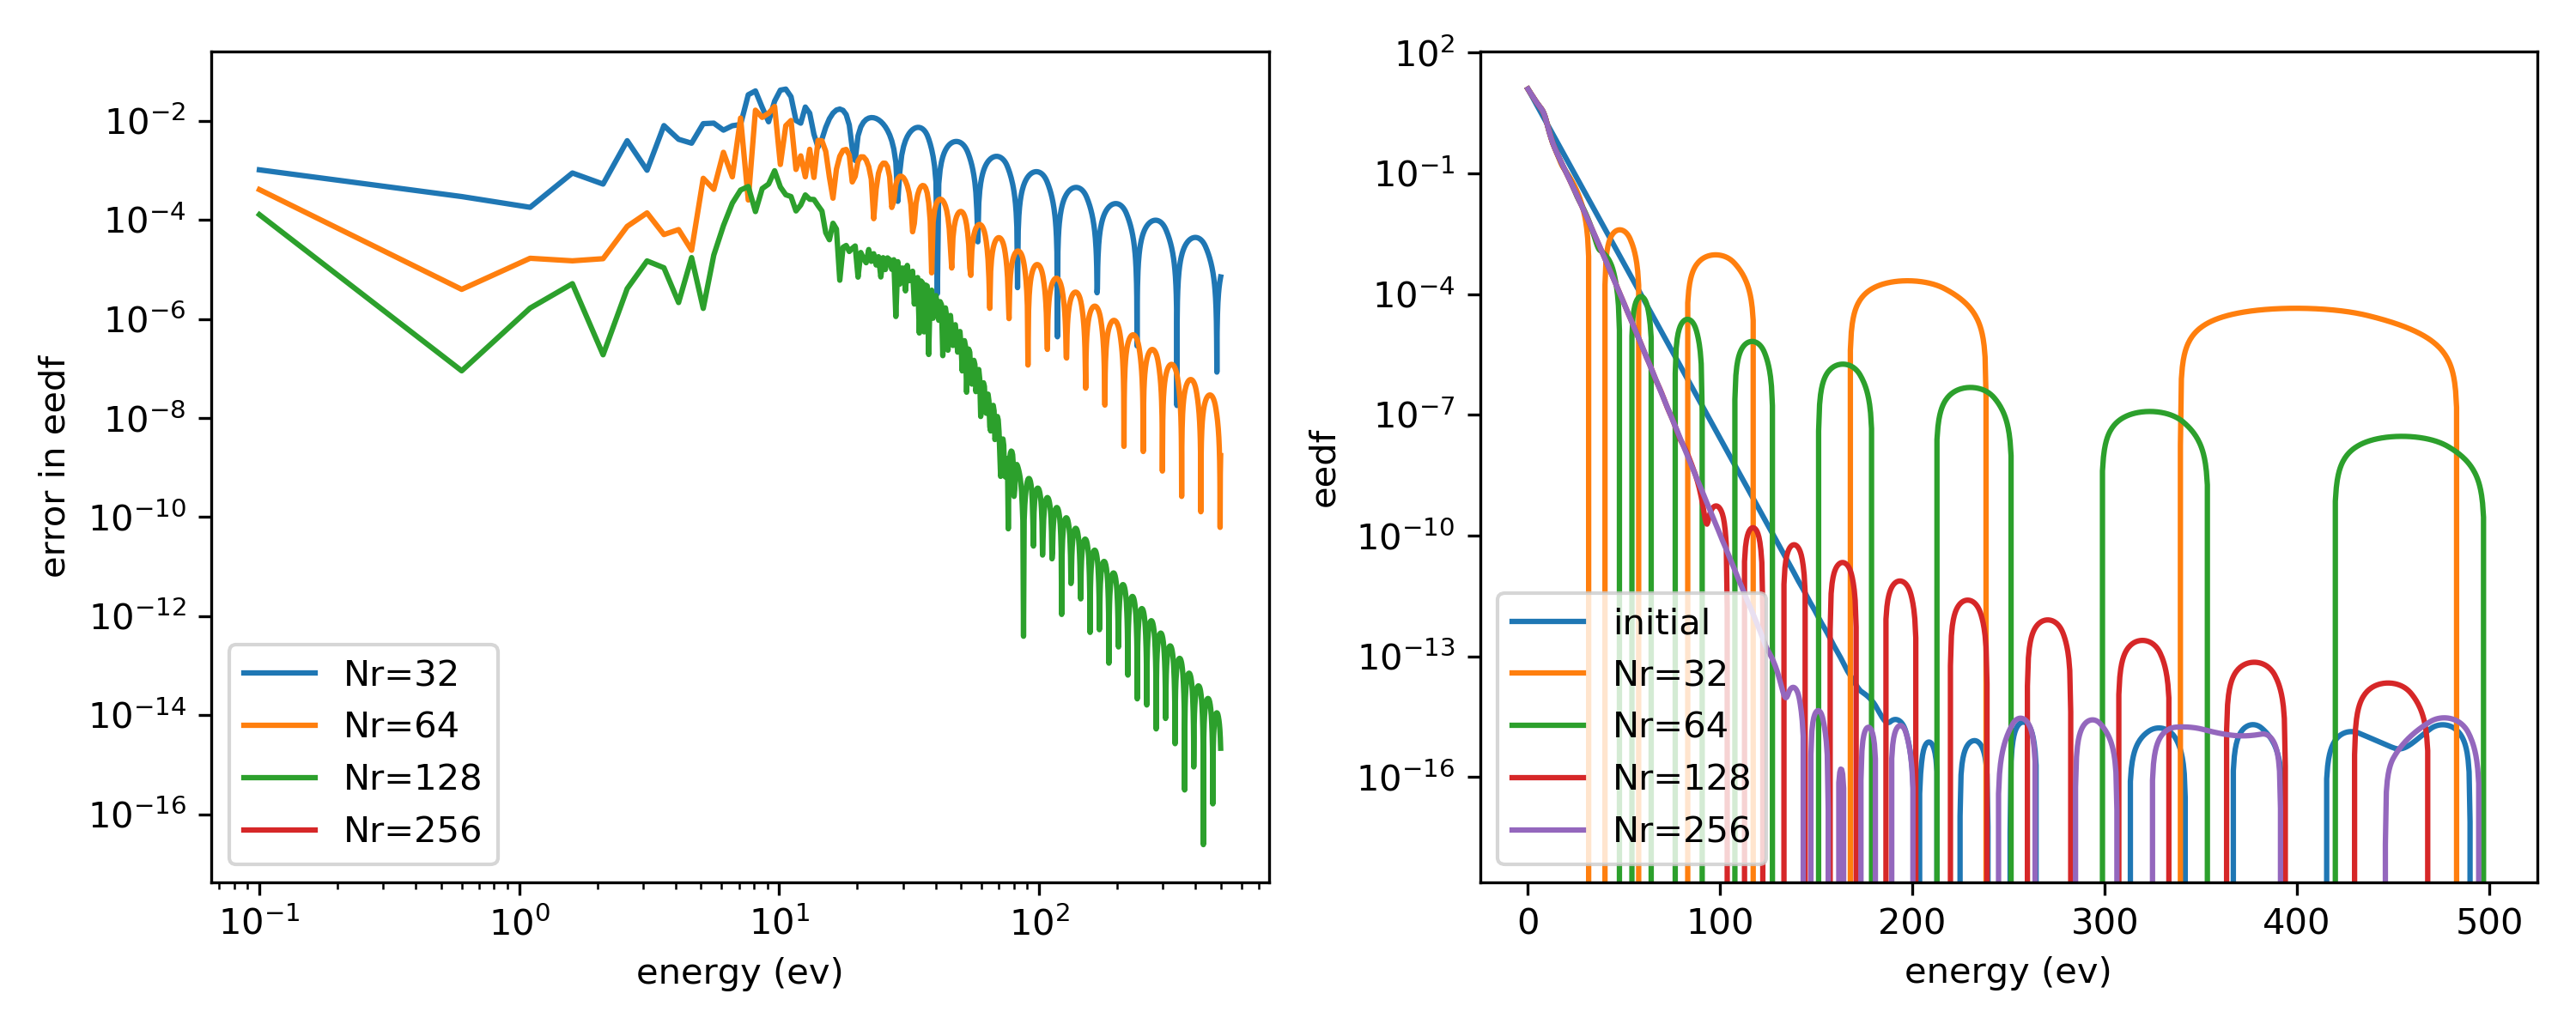
\includegraphics[width=0.48\textwidth]{figures/b_sp2_5ev_1e-6.png} 
		\end{tabular}
	\end{table}
	}
	
	\only<+>{
		Using Temp(t=0)=5eV, T=5e-6 s,
		\begin{table}
			\centering
			\begin{tabular}{cc}
				Maxwell &   quadratic splines\\
				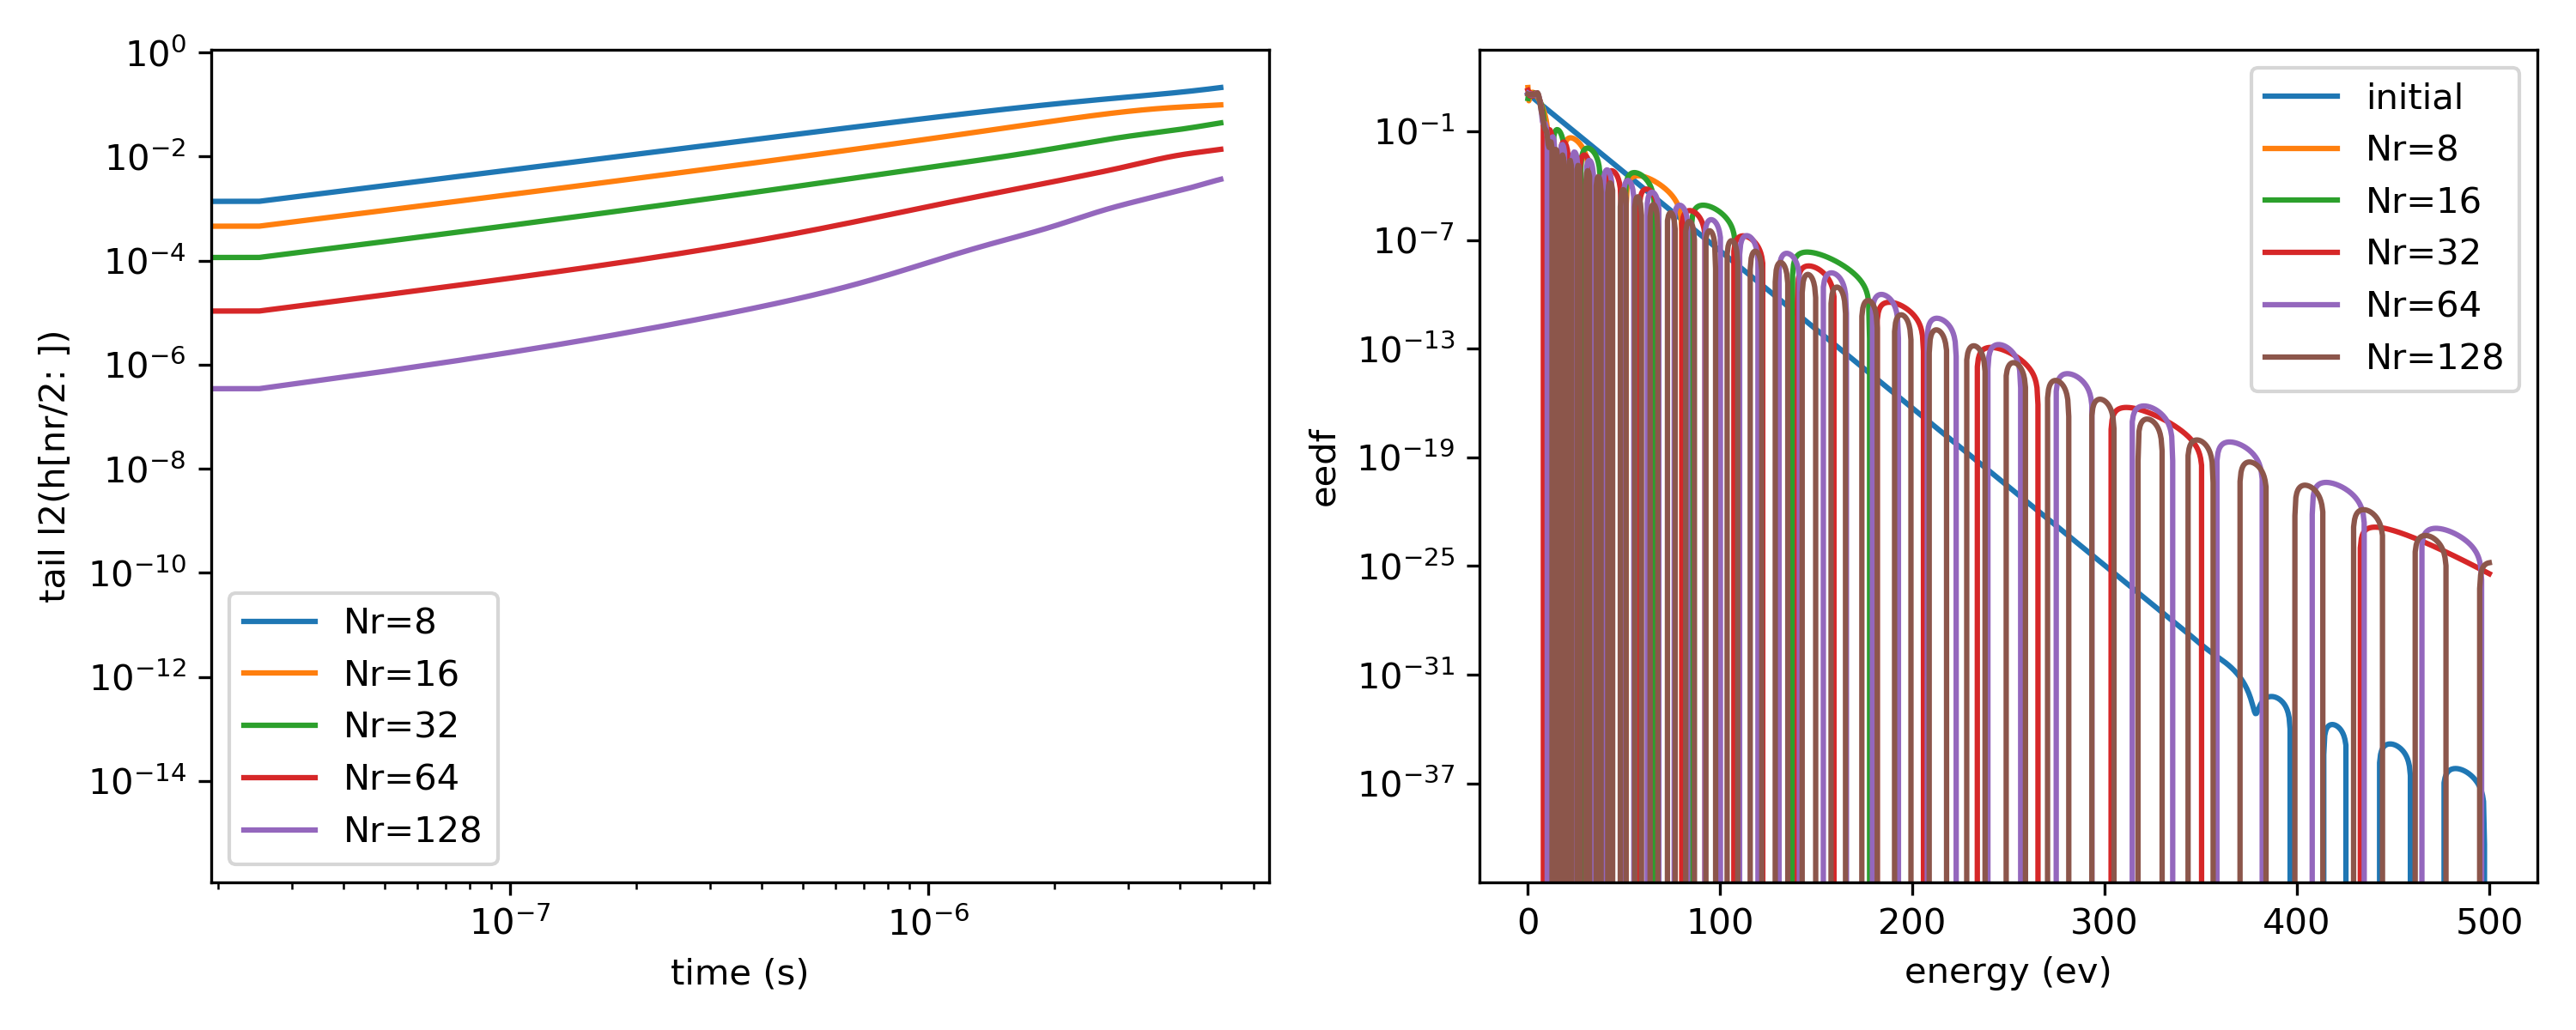
\includegraphics[width=0.48\textwidth]{figures/m_5ev_5e-6.png} & 
				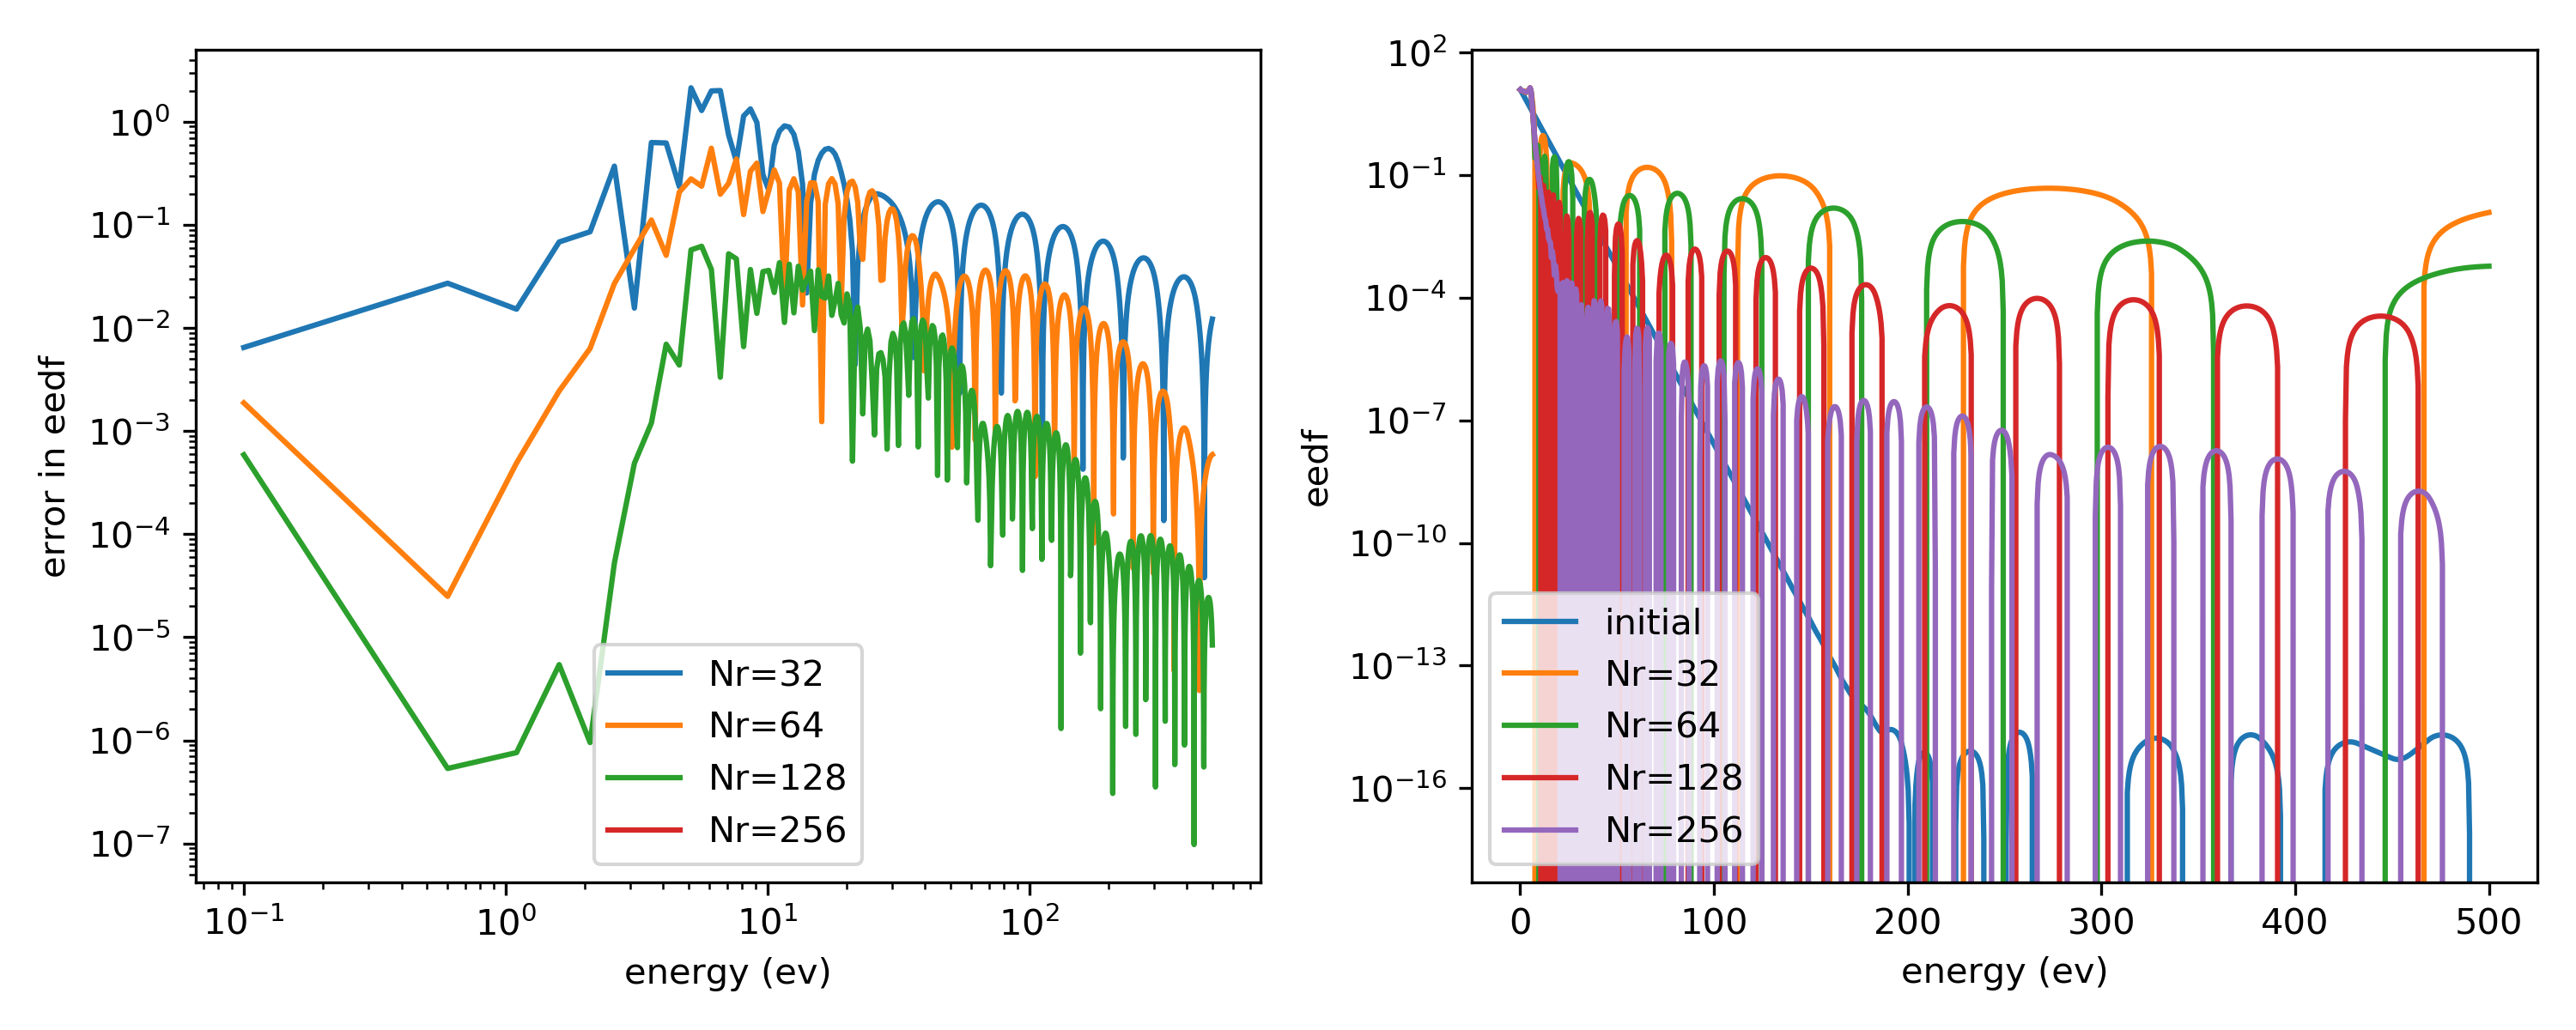
\includegraphics[width=0.48\textwidth]{figures/b_sp2_5ev_5e-6.png} 
			\end{tabular}
		\end{table}
	}
\end{frame}

\begin{frame}
	\frametitle{Accuracy tests}
	With elastic collisions without energy transfer and with angle independent differential cross section, isotropic distribution should stay isotropic during evolution. We start with $f(\vect{v},t=0) = M(\vect{v})$
	
	\begin{table}
		\centering
		\begin{tabular}{cc}
			Maxwell &   quadratic splines\\
			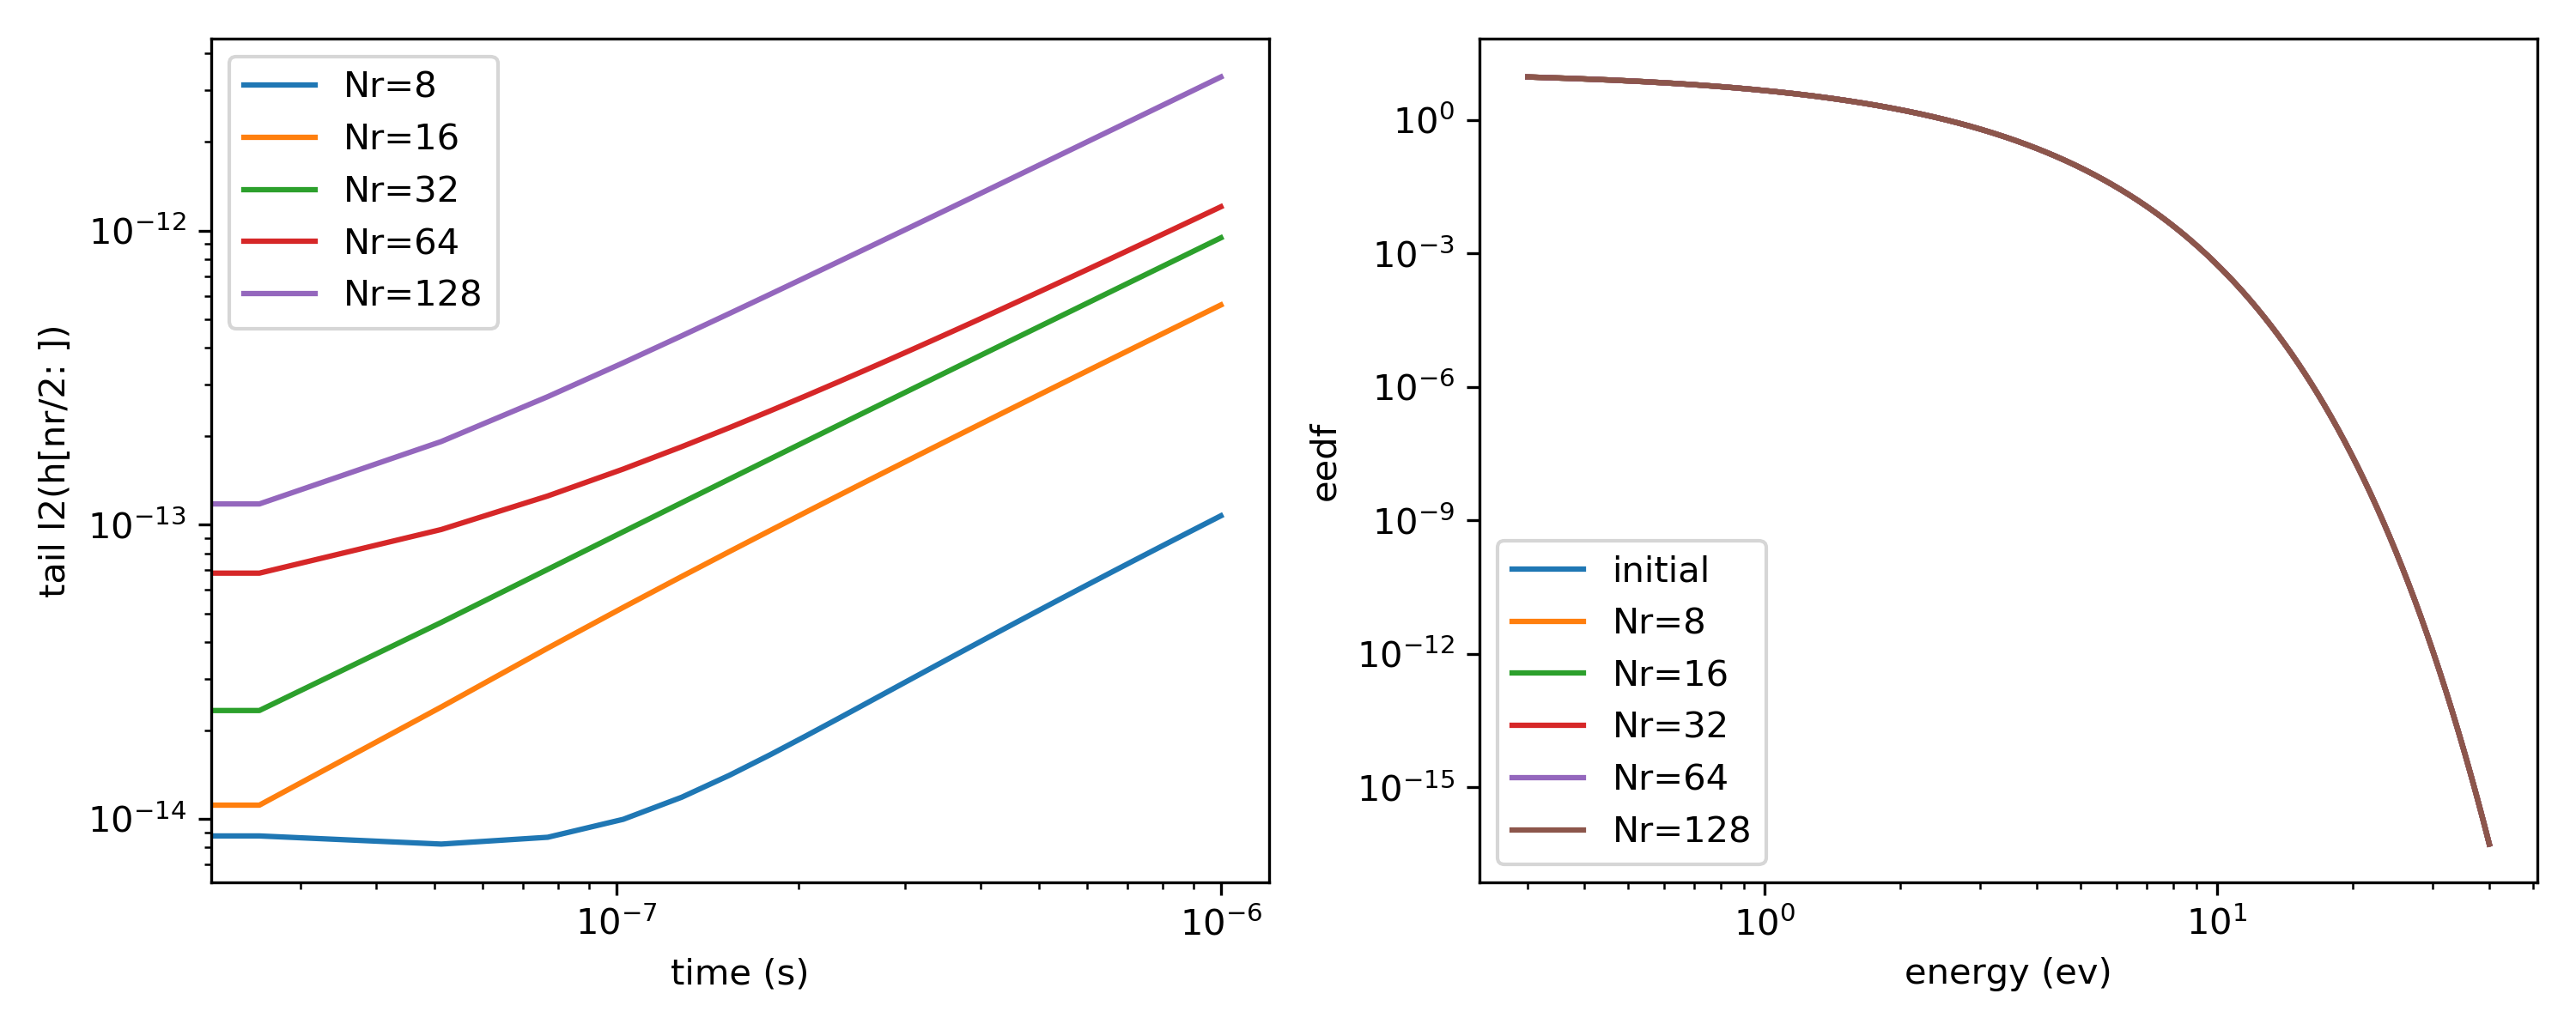
\includegraphics[width=0.48\textwidth]{figures/m_no_e_loss_1ev_1e-6.png} & 
			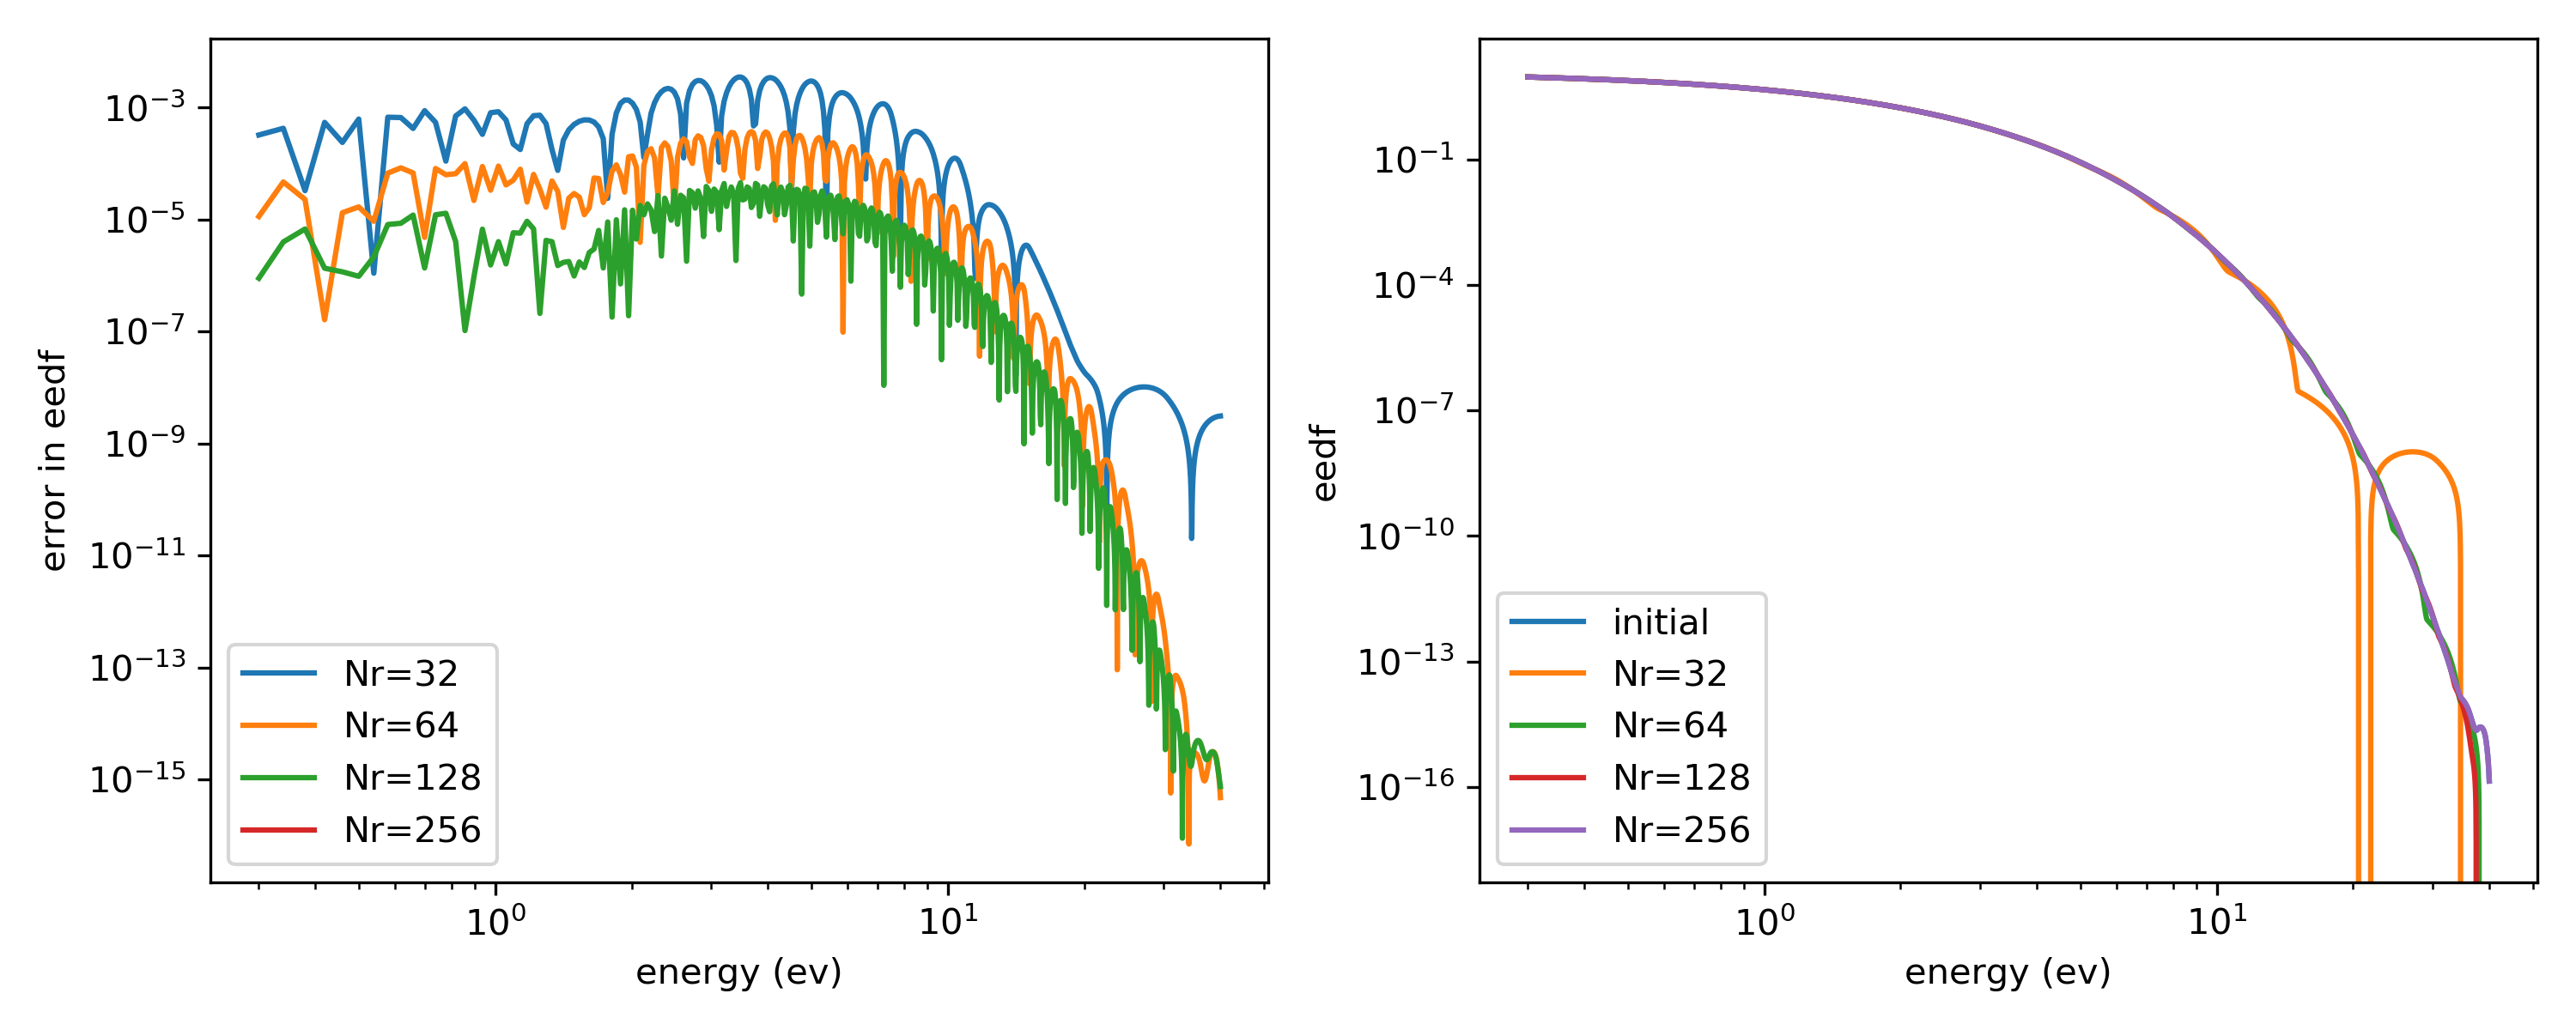
\includegraphics[width=0.48\textwidth]{figures/b_sp2_no_e_loss_1ev_1e-6.png} 
		\end{tabular}
	\end{table}
\end{frame}

\begin{frame}
	\frametitle{Accuracy tests}
	With elastic collisions without energy transfer and with angle independent differential cross section, if we start with anisotropic distribution we should reach isotropic distribution eventually. We start with $f(\vect{v},t=0) = M(\vect{v}) (1 + \tan v_\theta)$, evolved for time horizon T=4e-6 s.
	
	\only<+>
	{
		\begin{figure}
			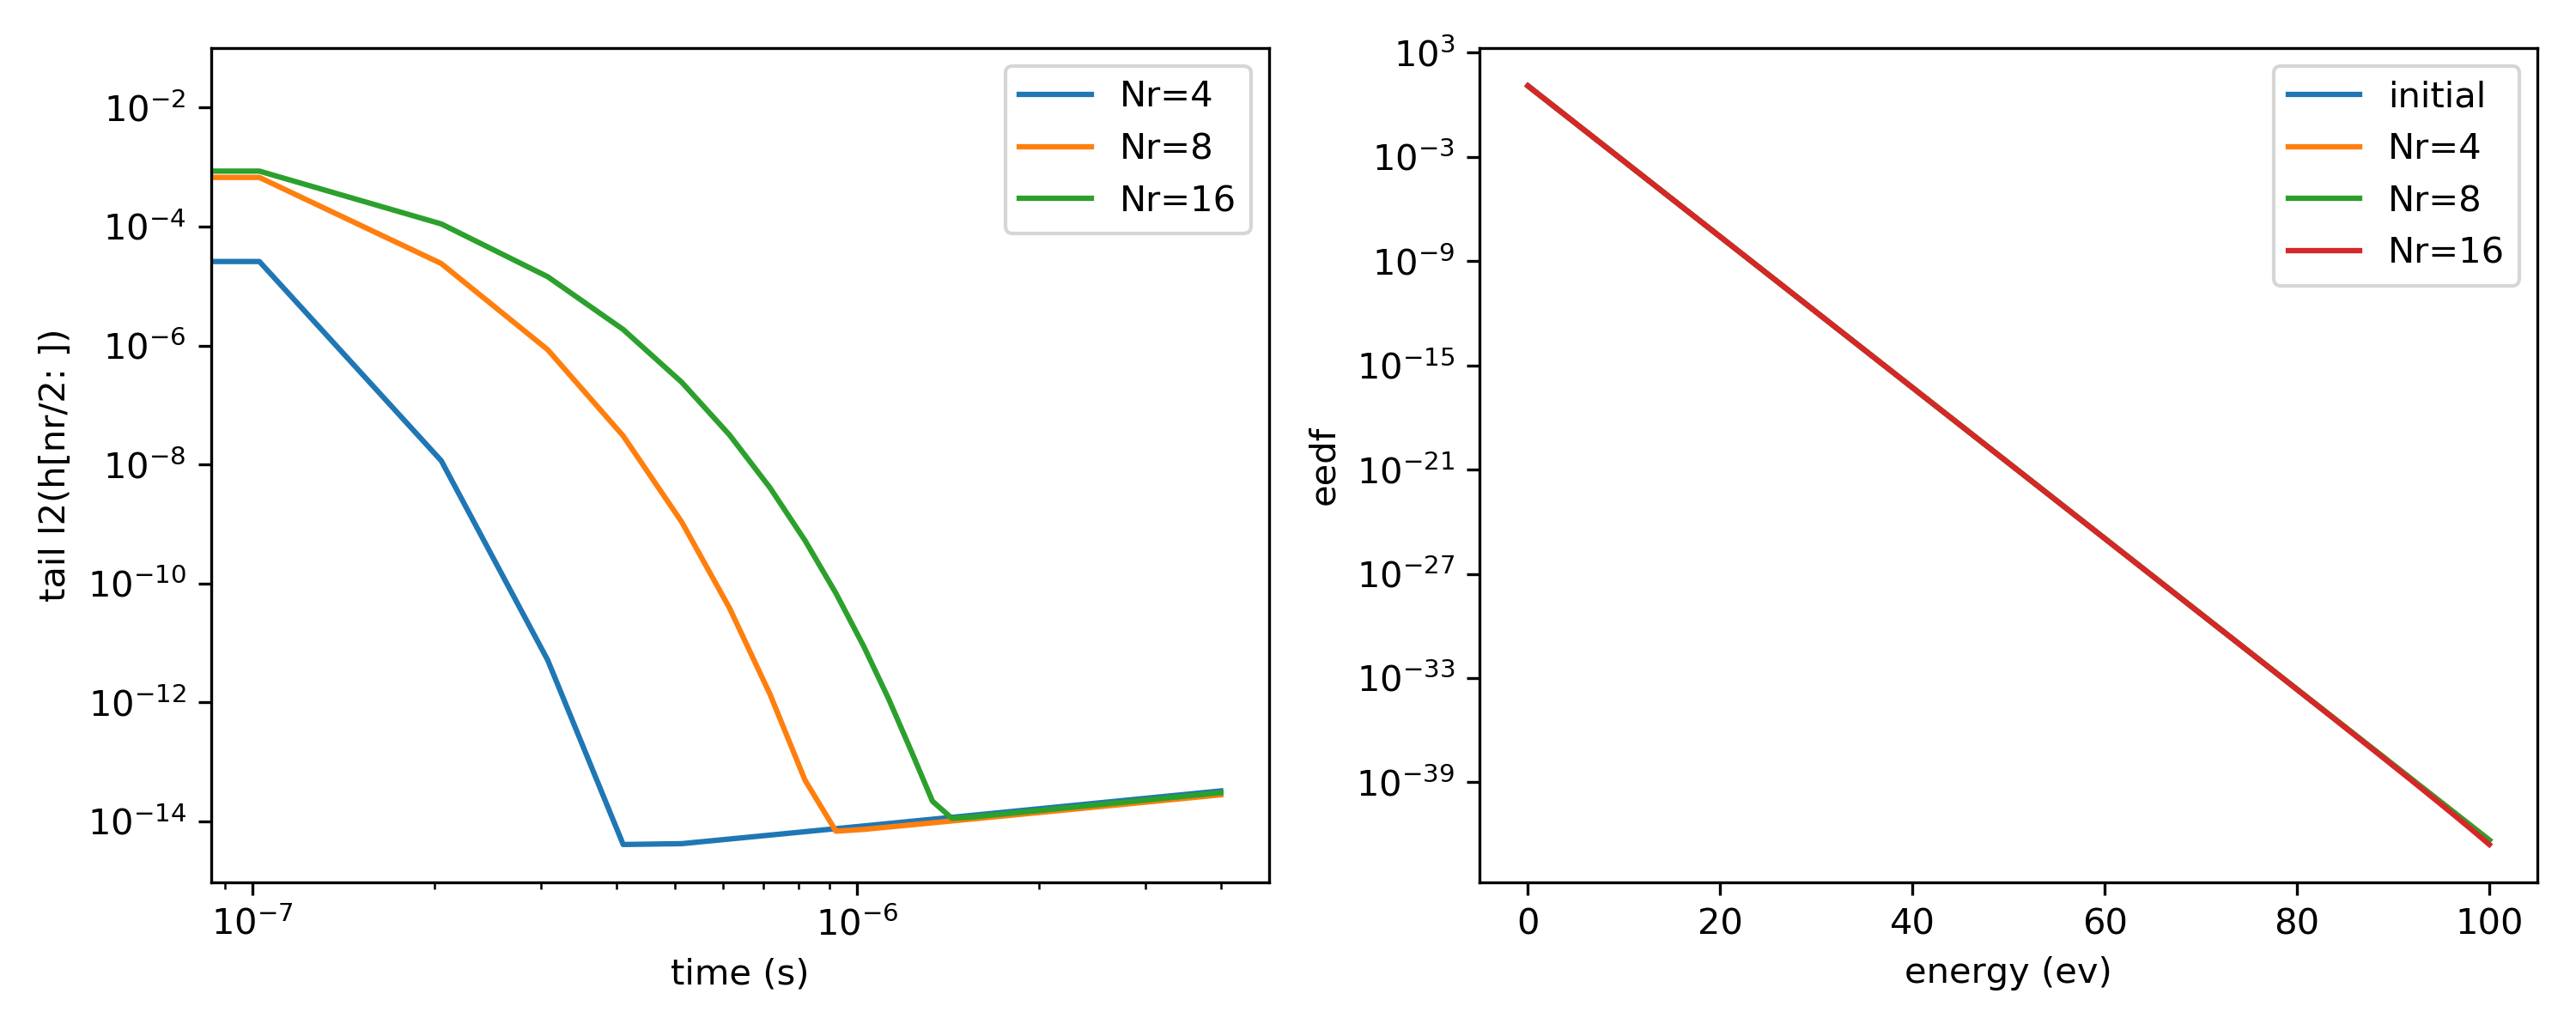
\includegraphics[width=0.8\textwidth]{figures/m_no_e_loss_aiso_test_1ev_4e-6_l2.png}
		\end{figure}
	}
	\only<+>
	{
		\begin{figure}
			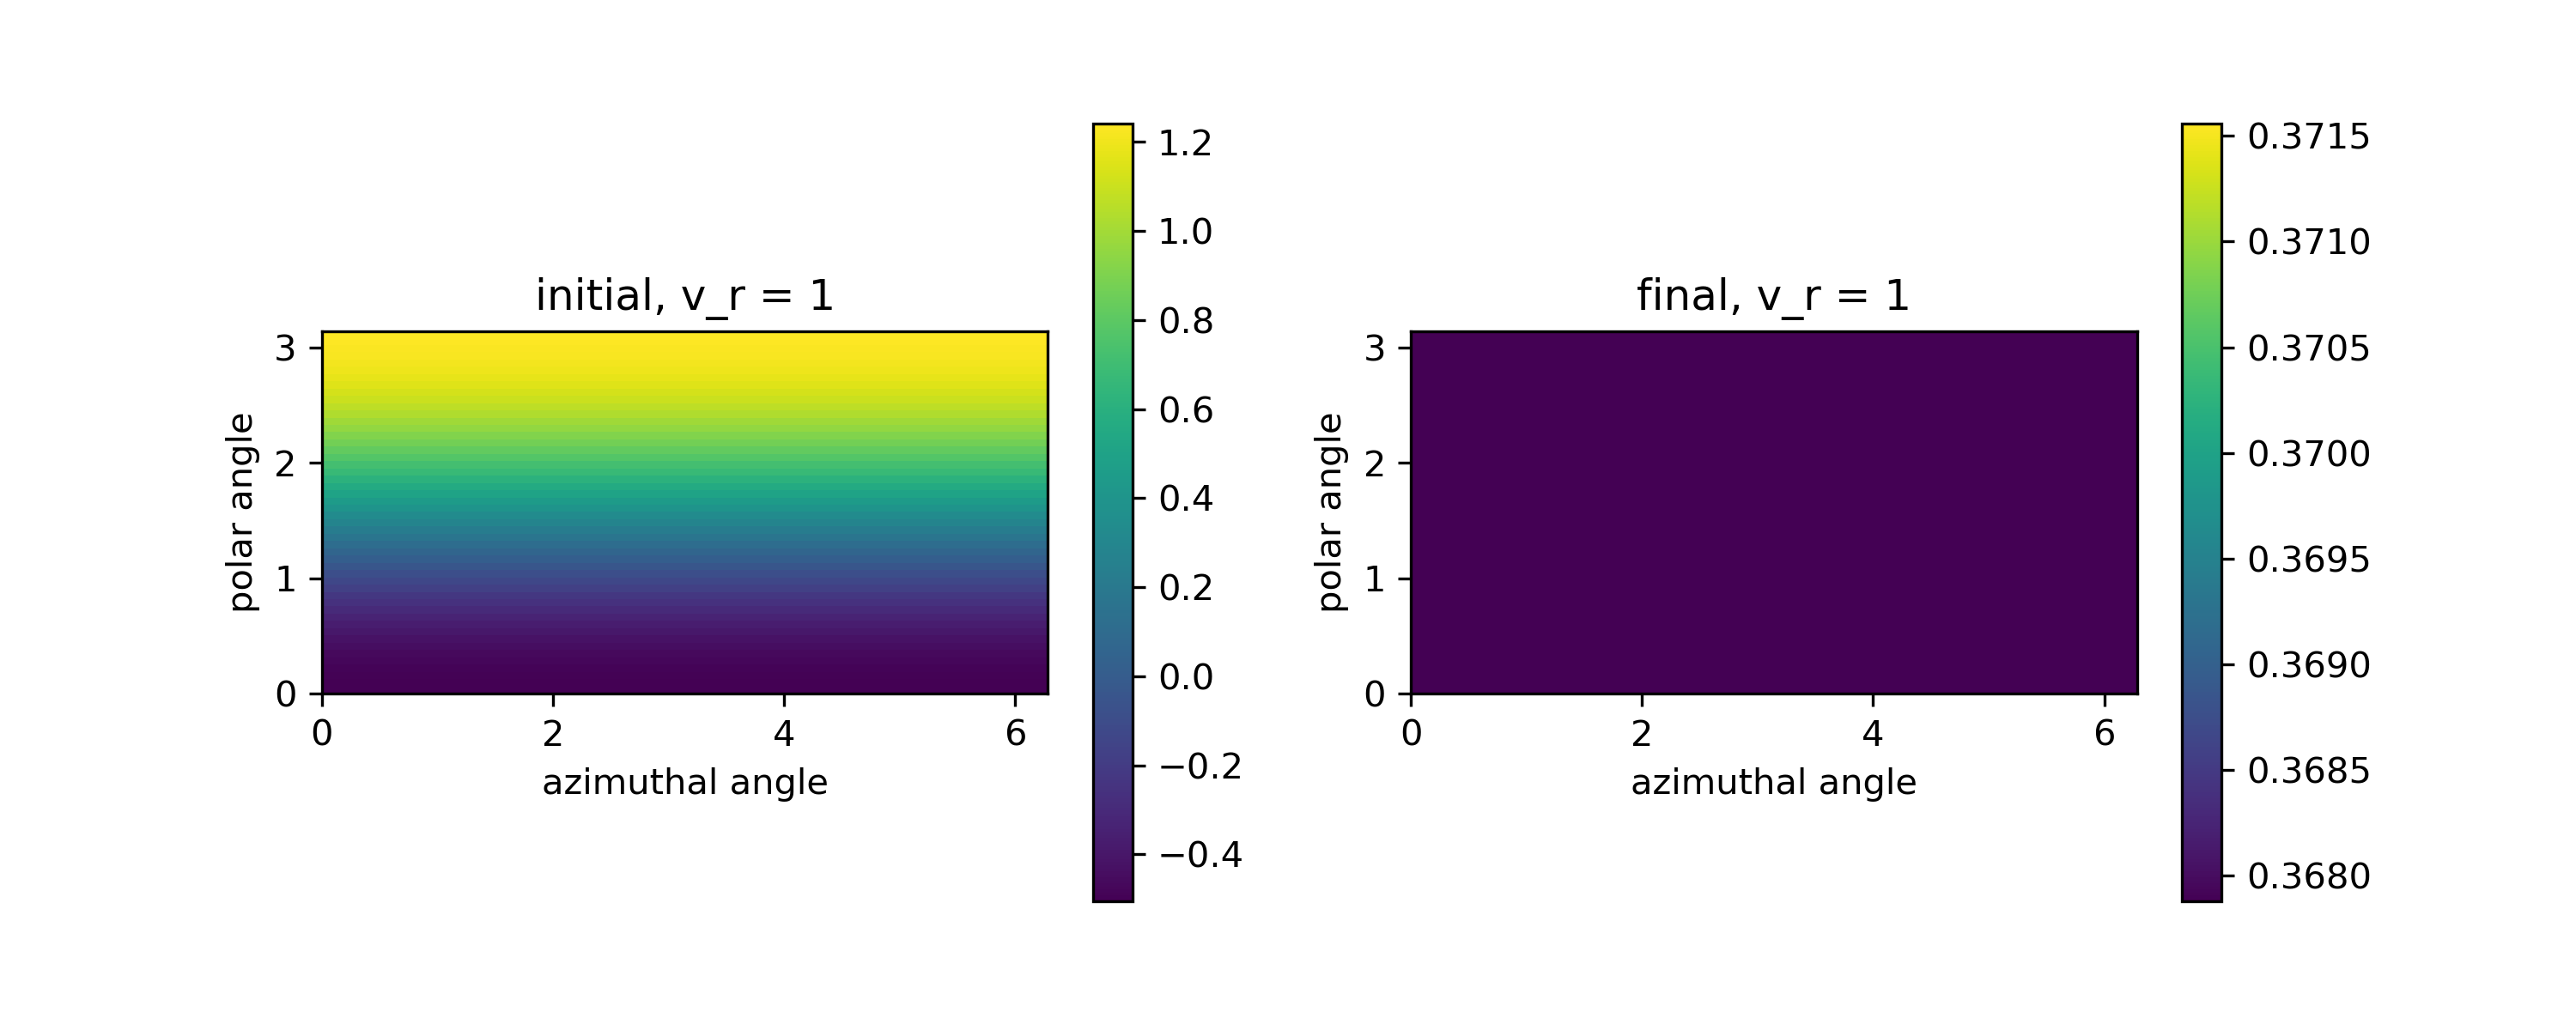
\includegraphics[width=0.8\textwidth]{figures/m_no_e_loss_aiso_test_1ev_4e-6_l2_const_r.png}
		\end{figure}
	}
\end{frame}


\begin{frame}{Changing expansion thermal velocity}
	Let $\beta$ be the chosen thermal velocity for the $f(\vect{v})$ expansion, $\alpha$ be the actual thermal velocity (i.e., for corresponding temperature).
	\begin{align*}
		f(\vect{v},0) &= \frac{n_e}{(\sqrt{\pi}\alpha)^3}\exp\of{-\frac{v_r^2}{\alpha^2}} = \underbrace{\frac{n_e}{(\sqrt{\pi}\beta)^3} \exp\of{-\frac{v_r^2}{\beta^2}}}_{M(\vect{v})} \underbrace{\left(\frac{\beta}{\alpha}\right)^3 \exp\of{-\frac{v_r^2}{\alpha^2} + \frac{v_r^2}{\beta^2}}}_{h(\vect{v})} 
	\end{align*}
\end{frame}

\begin{frame}{Maxwell polynomials with $\beta=\lambda \alpha$}
	\begin{center}
		\only<+>{
		chosen $\beta = 1.0 \alpha$
		\begin{figure}
			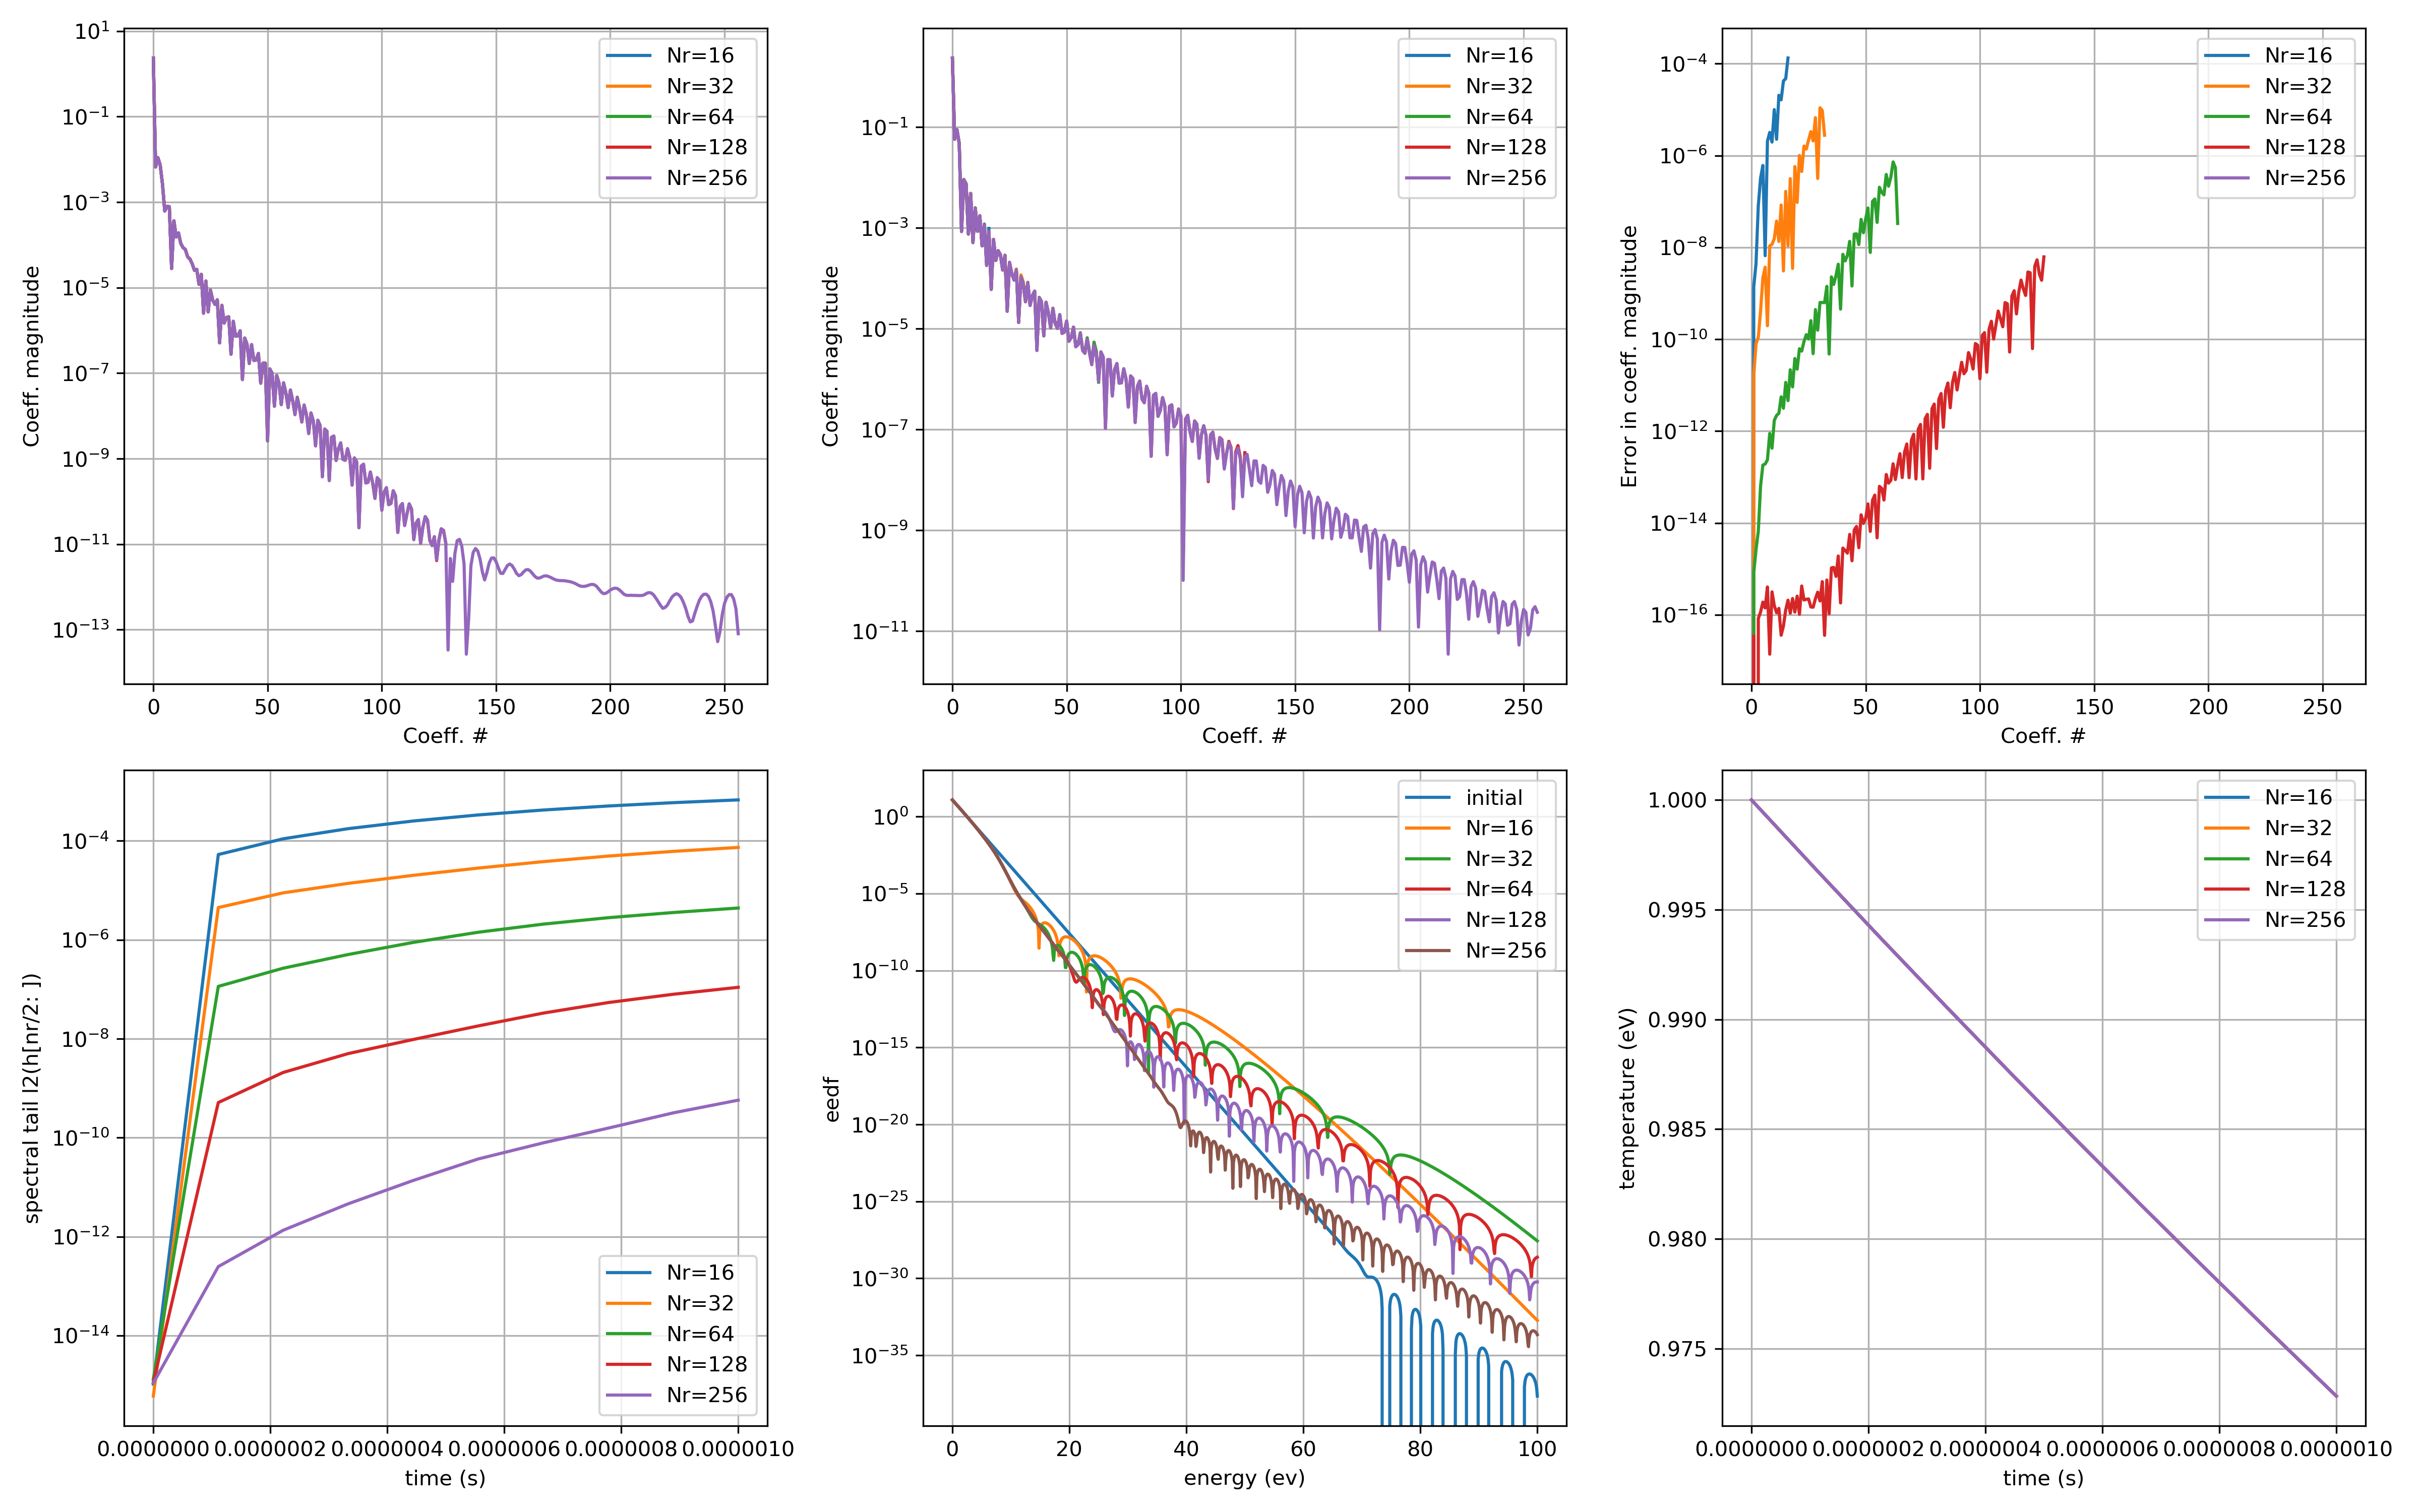
\includegraphics[width=0.6\textwidth]{figures/m_1ev_1e0vth_coeff.png}
		\end{figure}
		}
		\only<+>{
		chosen $\beta = 0.9 \alpha$
		\begin{figure}
		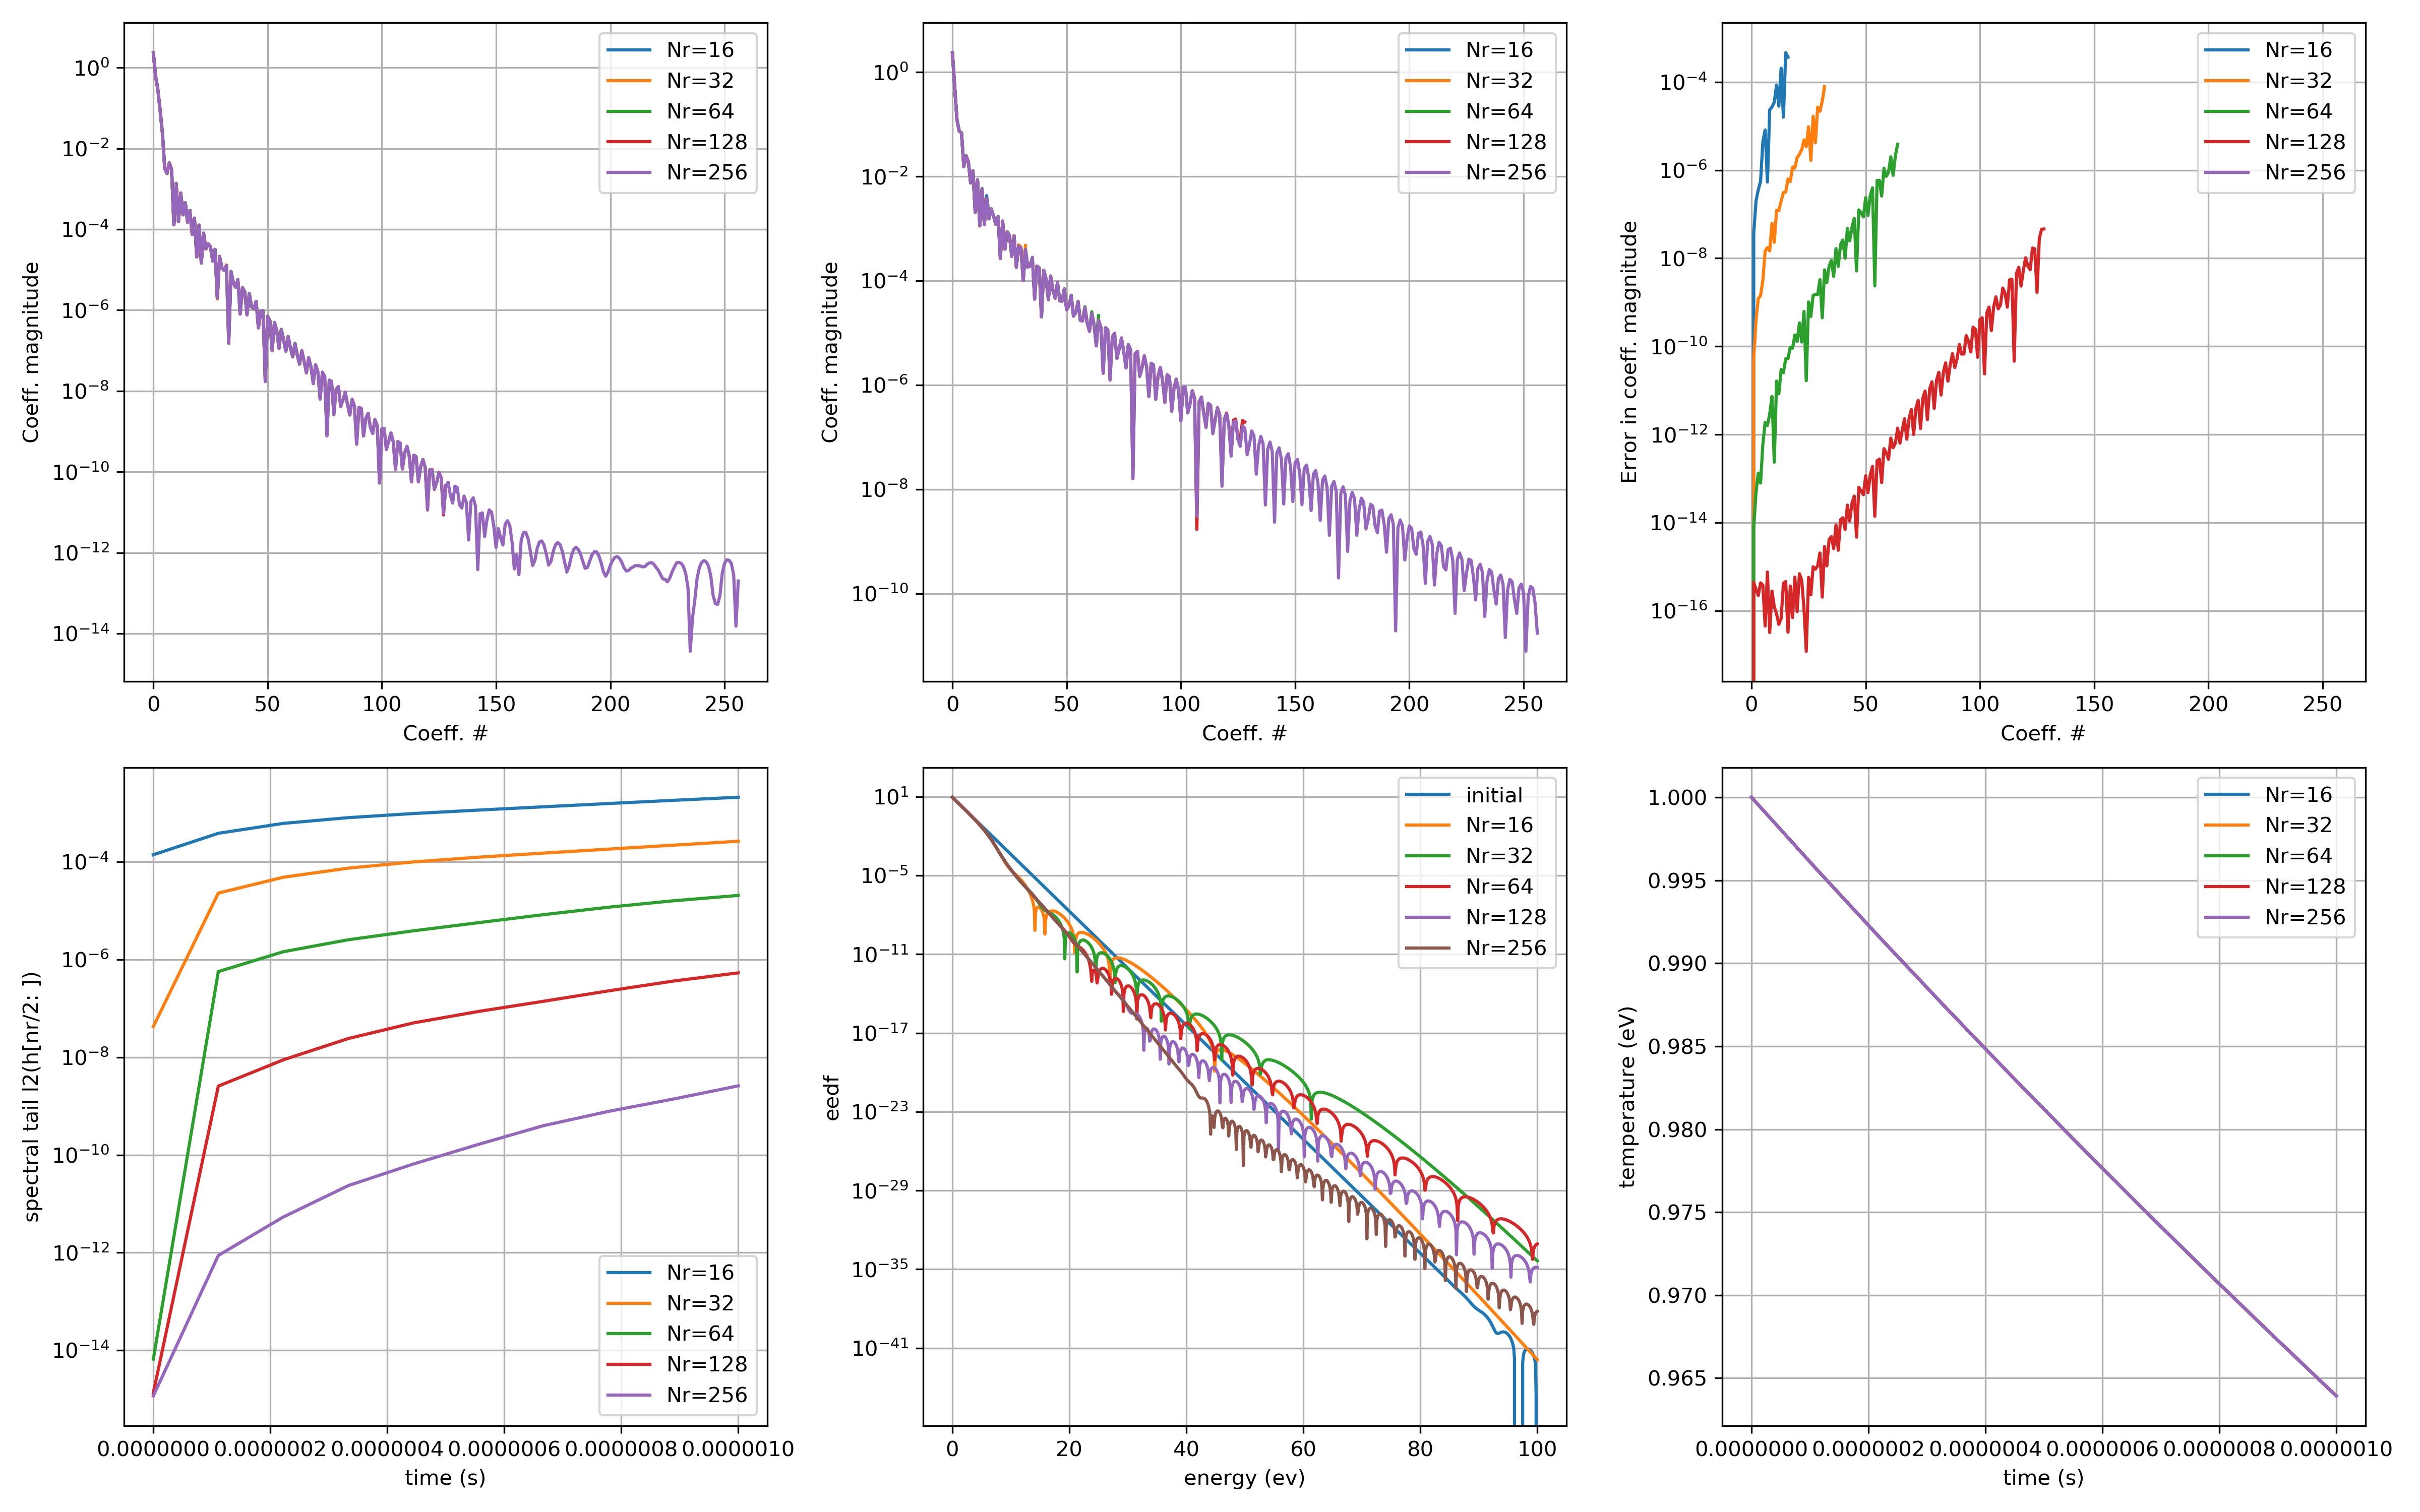
\includegraphics[width=0.6\textwidth]{figures/m_1ev_9e-1vth_coeff.png}
		\end{figure}
		}
		\only<+>{
		chosen $\beta = 0.8 \alpha$
		\begin{figure}
		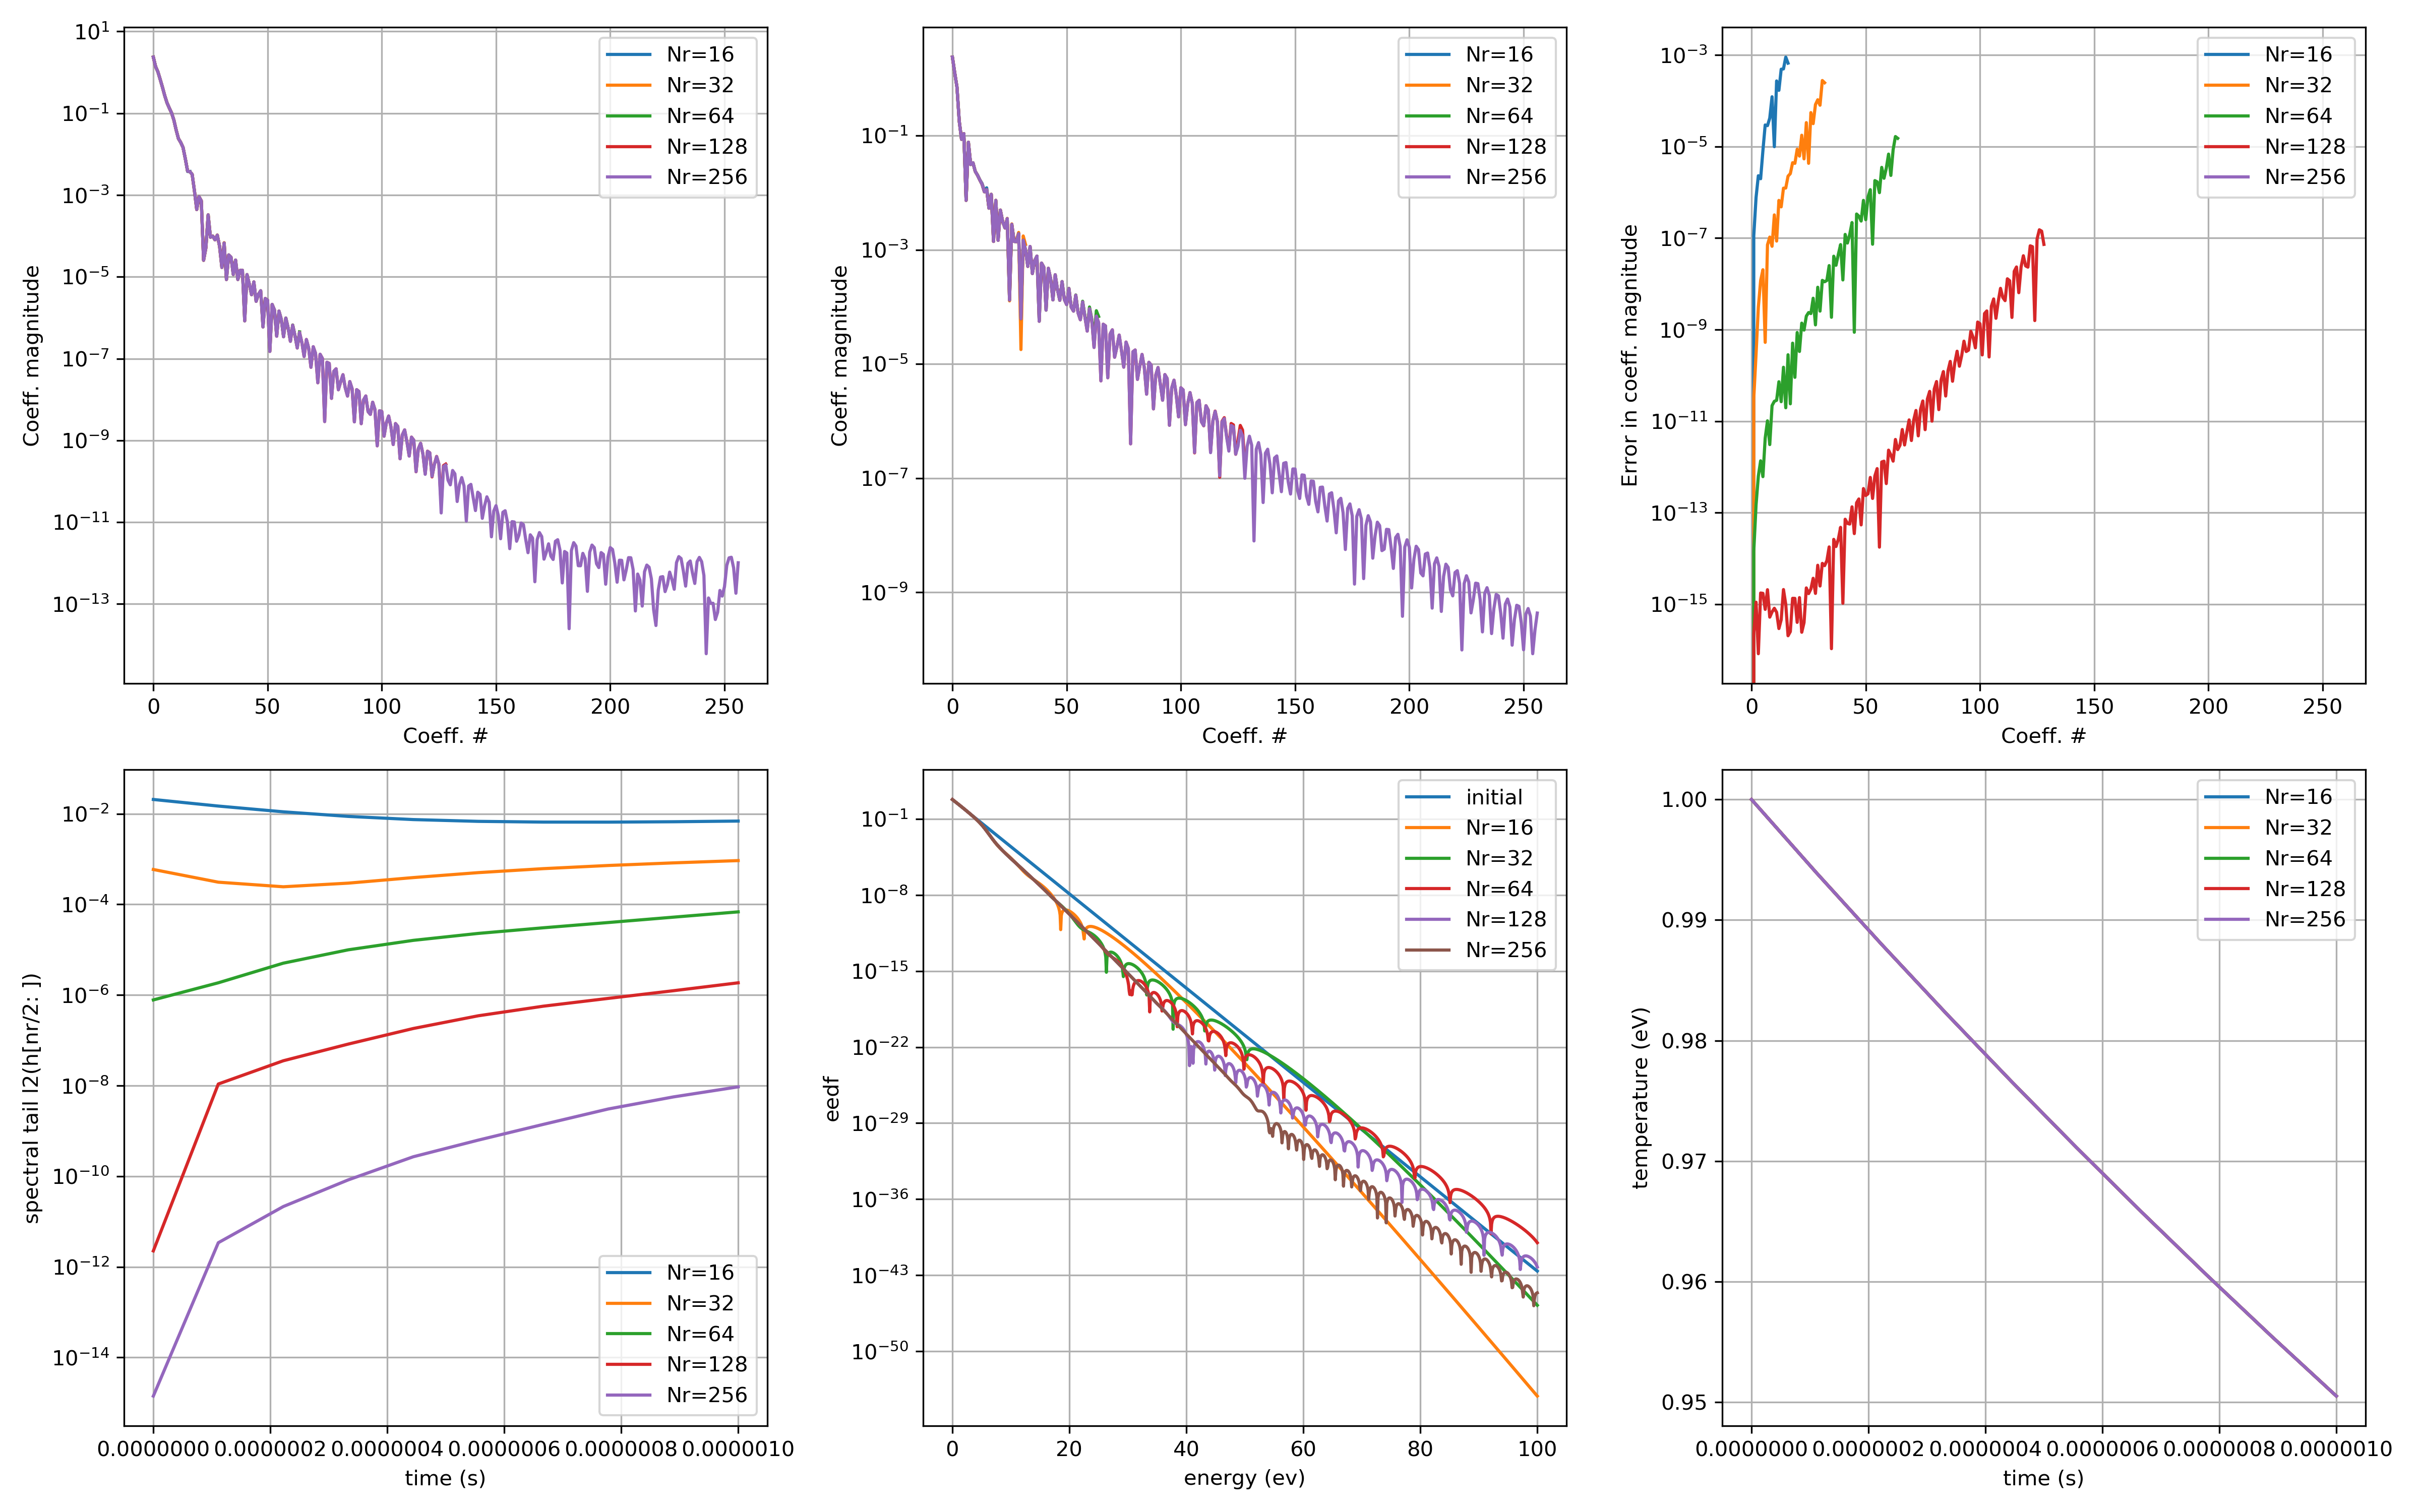
\includegraphics[width=0.6\textwidth]{figures/m_1ev_8e-1vth_coeff.png}
		\end{figure}

		}
		\only<+>{
		chosen $\beta = 0.7 \alpha$
		\begin{figure}
		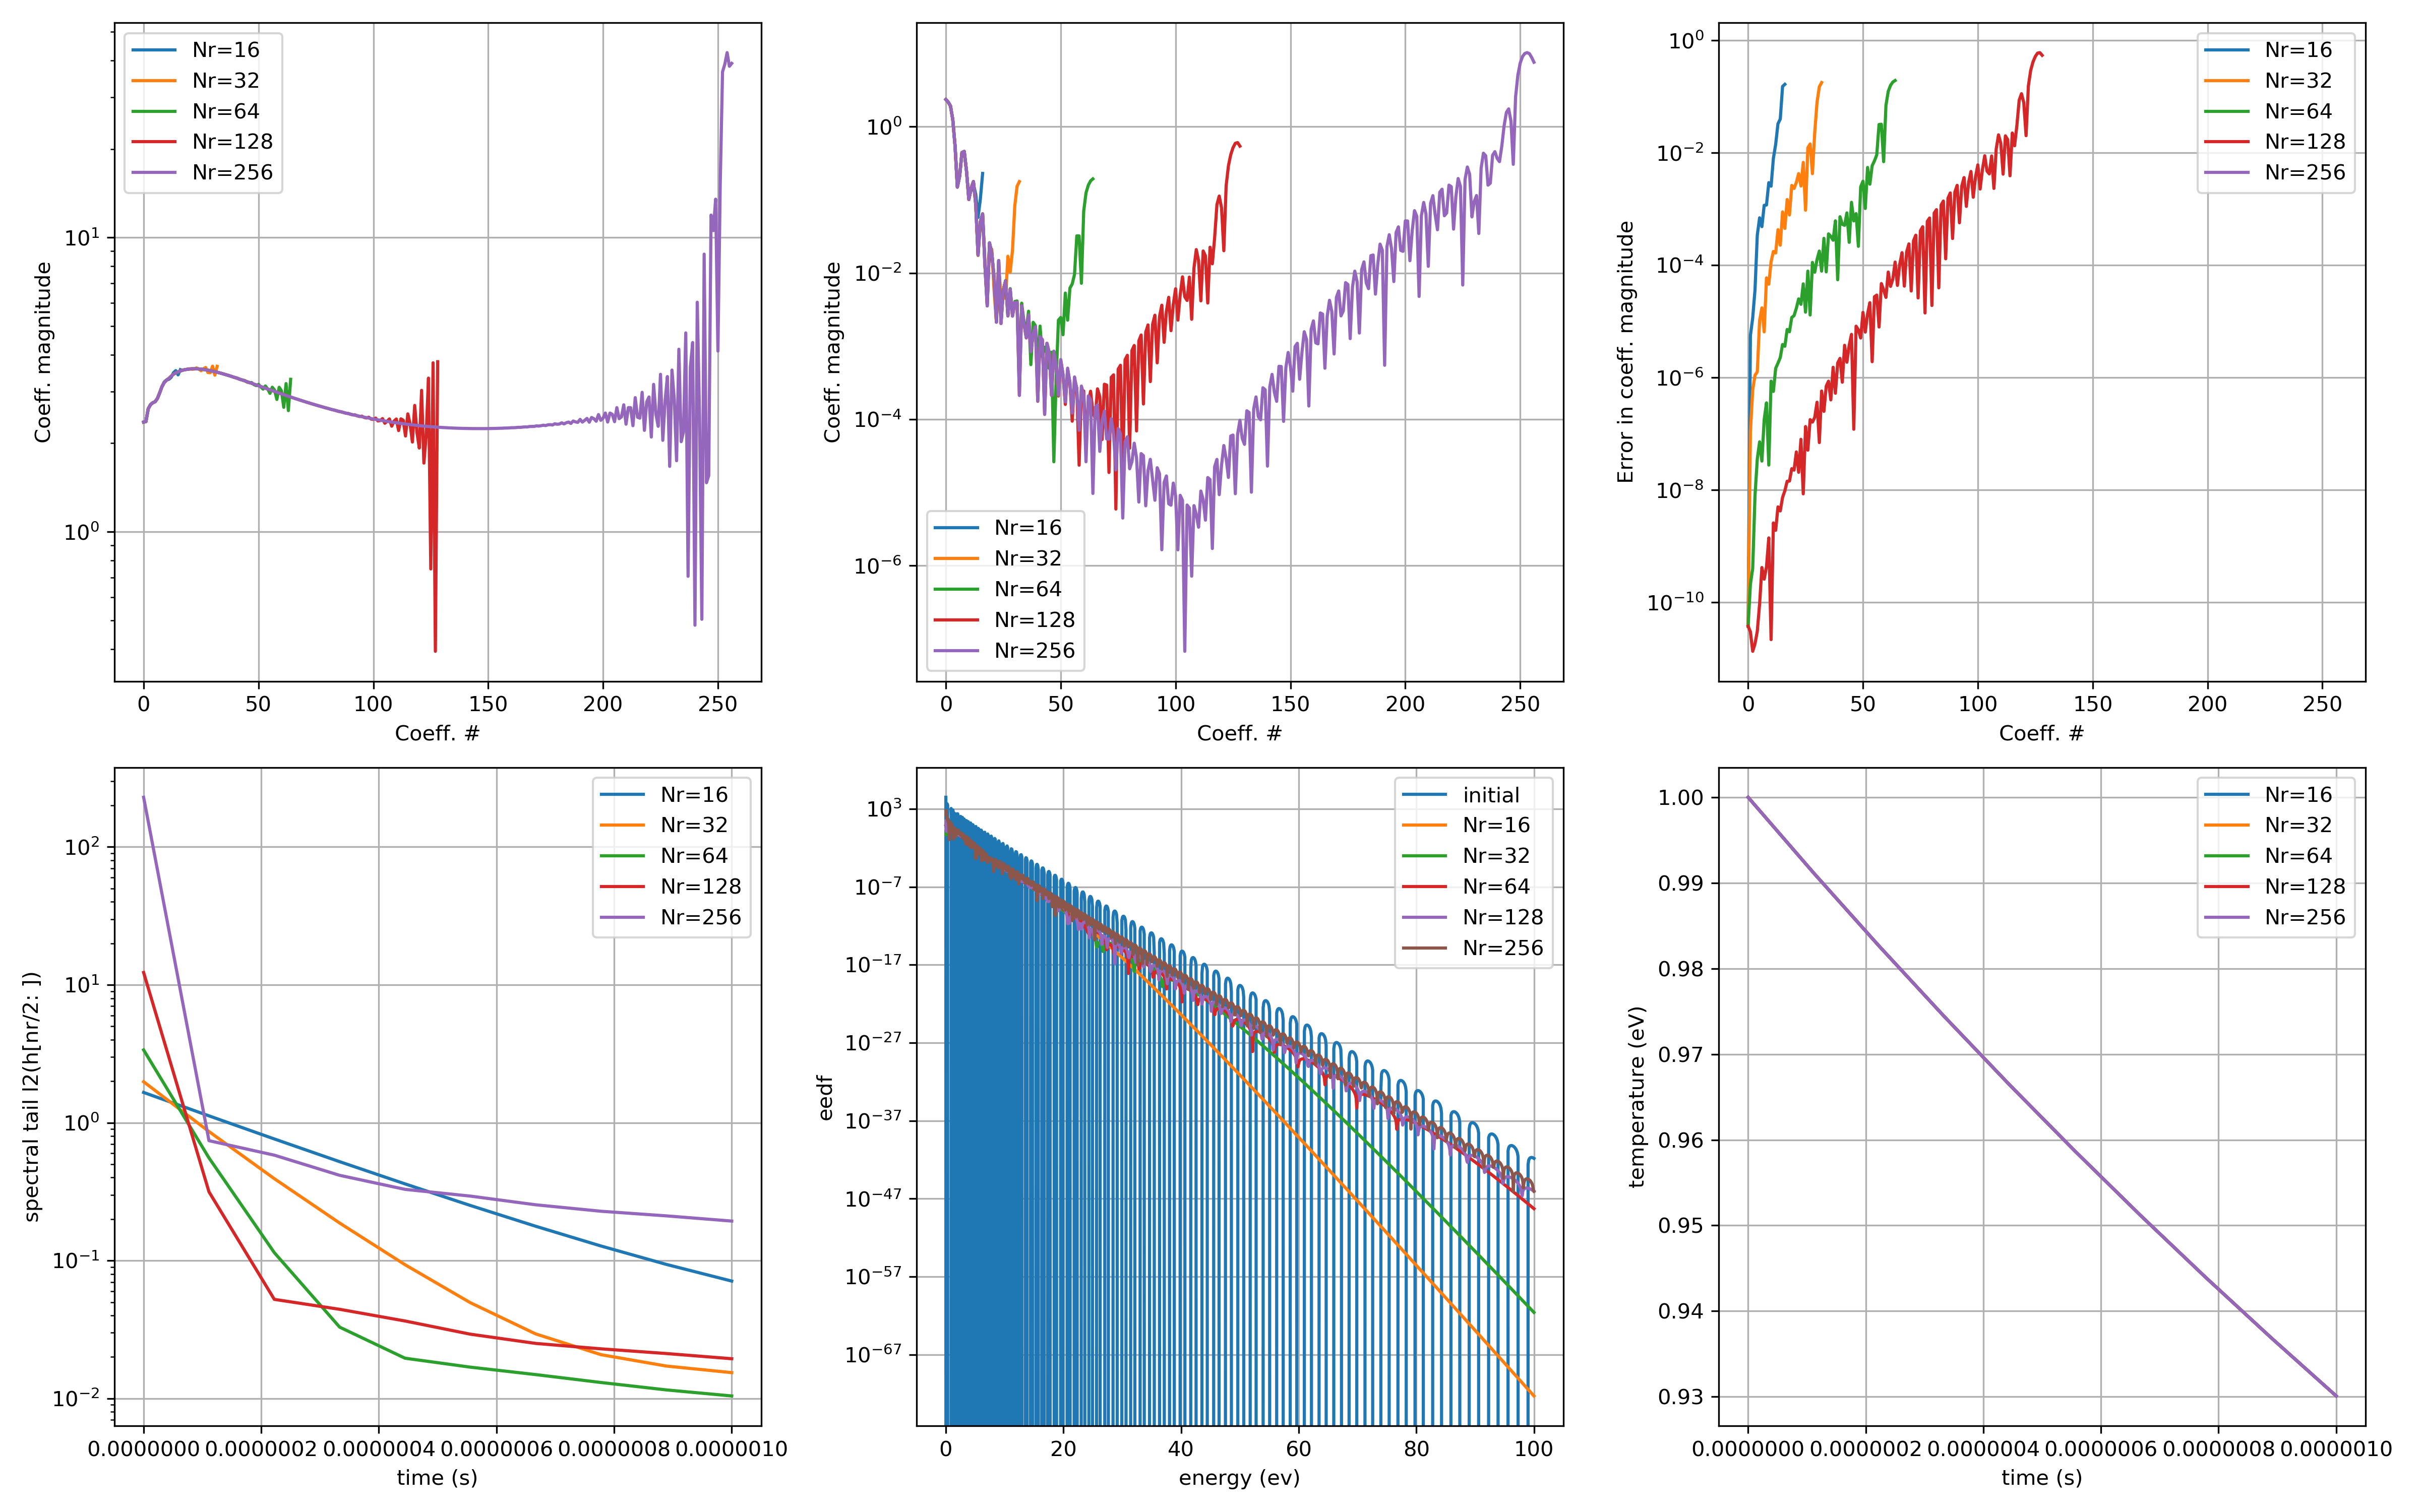
\includegraphics[width=0.6\textwidth]{figures/m_1ev_7e-1vth_coeff.png}
		\end{figure}
		}
	\end{center}
\end{frame}

\begin{frame}{Quadratic splines with $\beta=\lambda \alpha$}
	\begin{center}
		\only<+>{
			chosen $\beta = 1.0 \alpha$
			\begin{figure}
				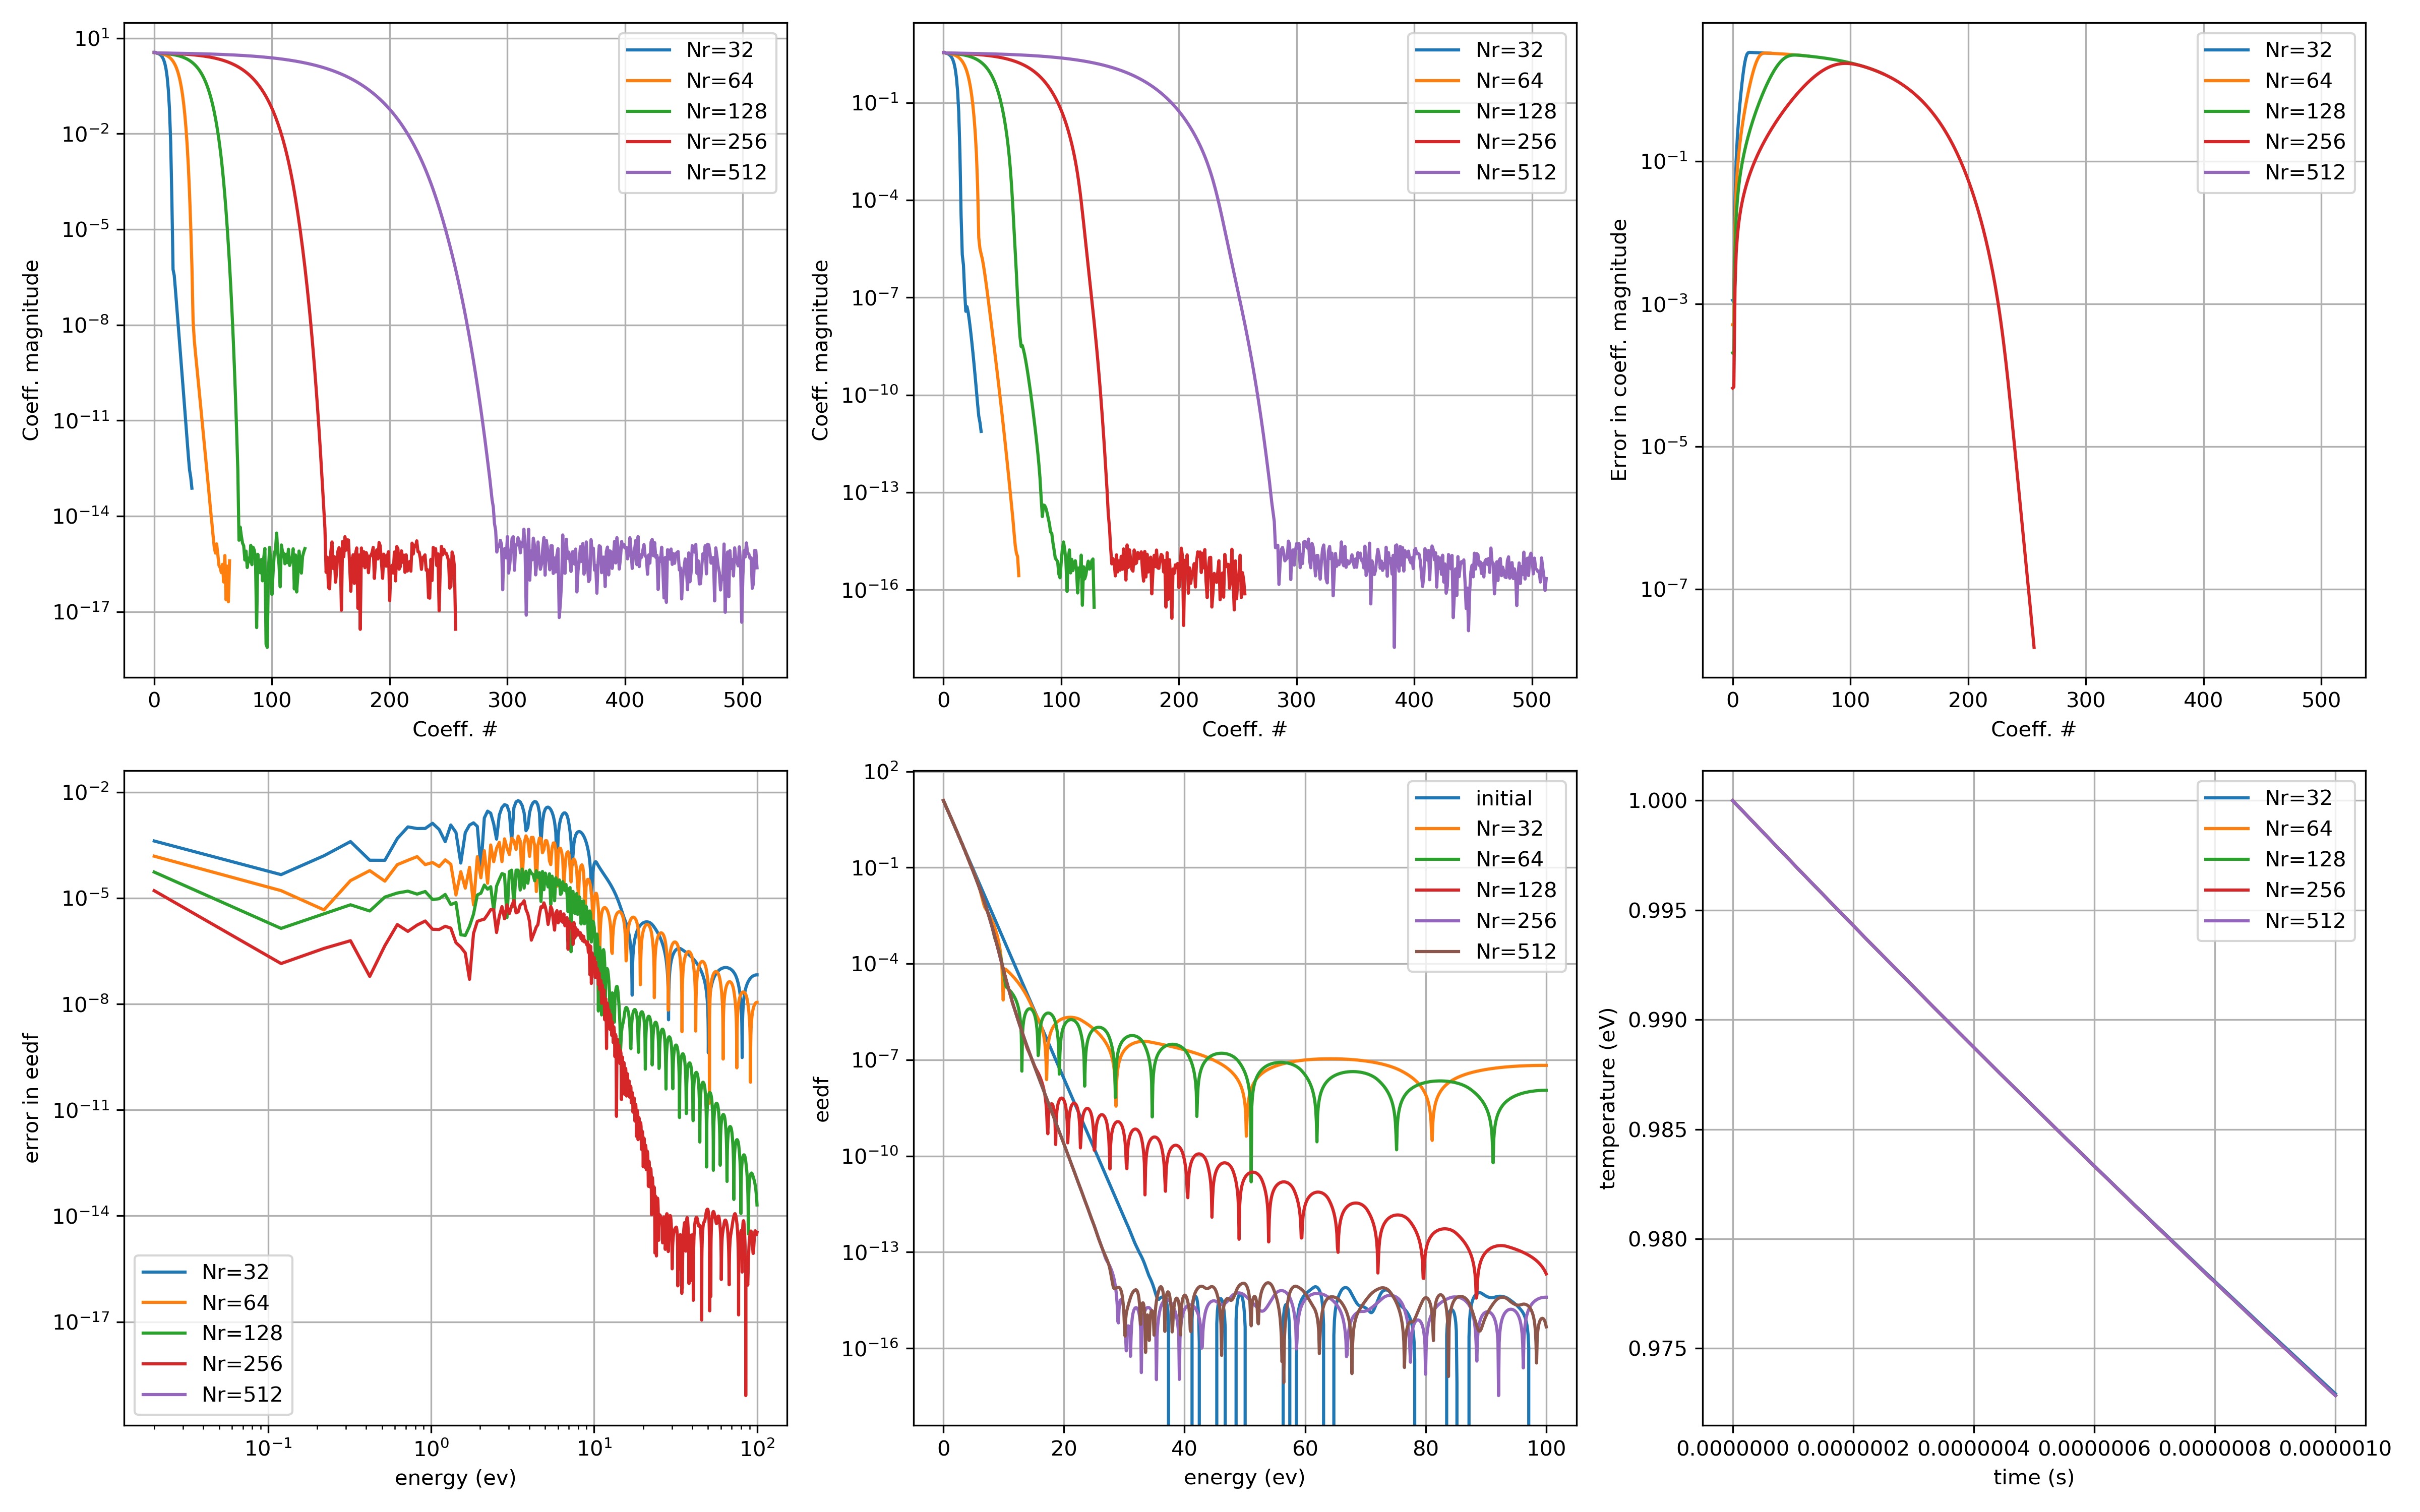
\includegraphics[width=0.6\textwidth]{figures/b_sp2_1ev_1e0vth_coeff.png}
			\end{figure}
		}
		\only<+>{
			chosen $\beta = 0.98 \alpha$
			\begin{figure}
				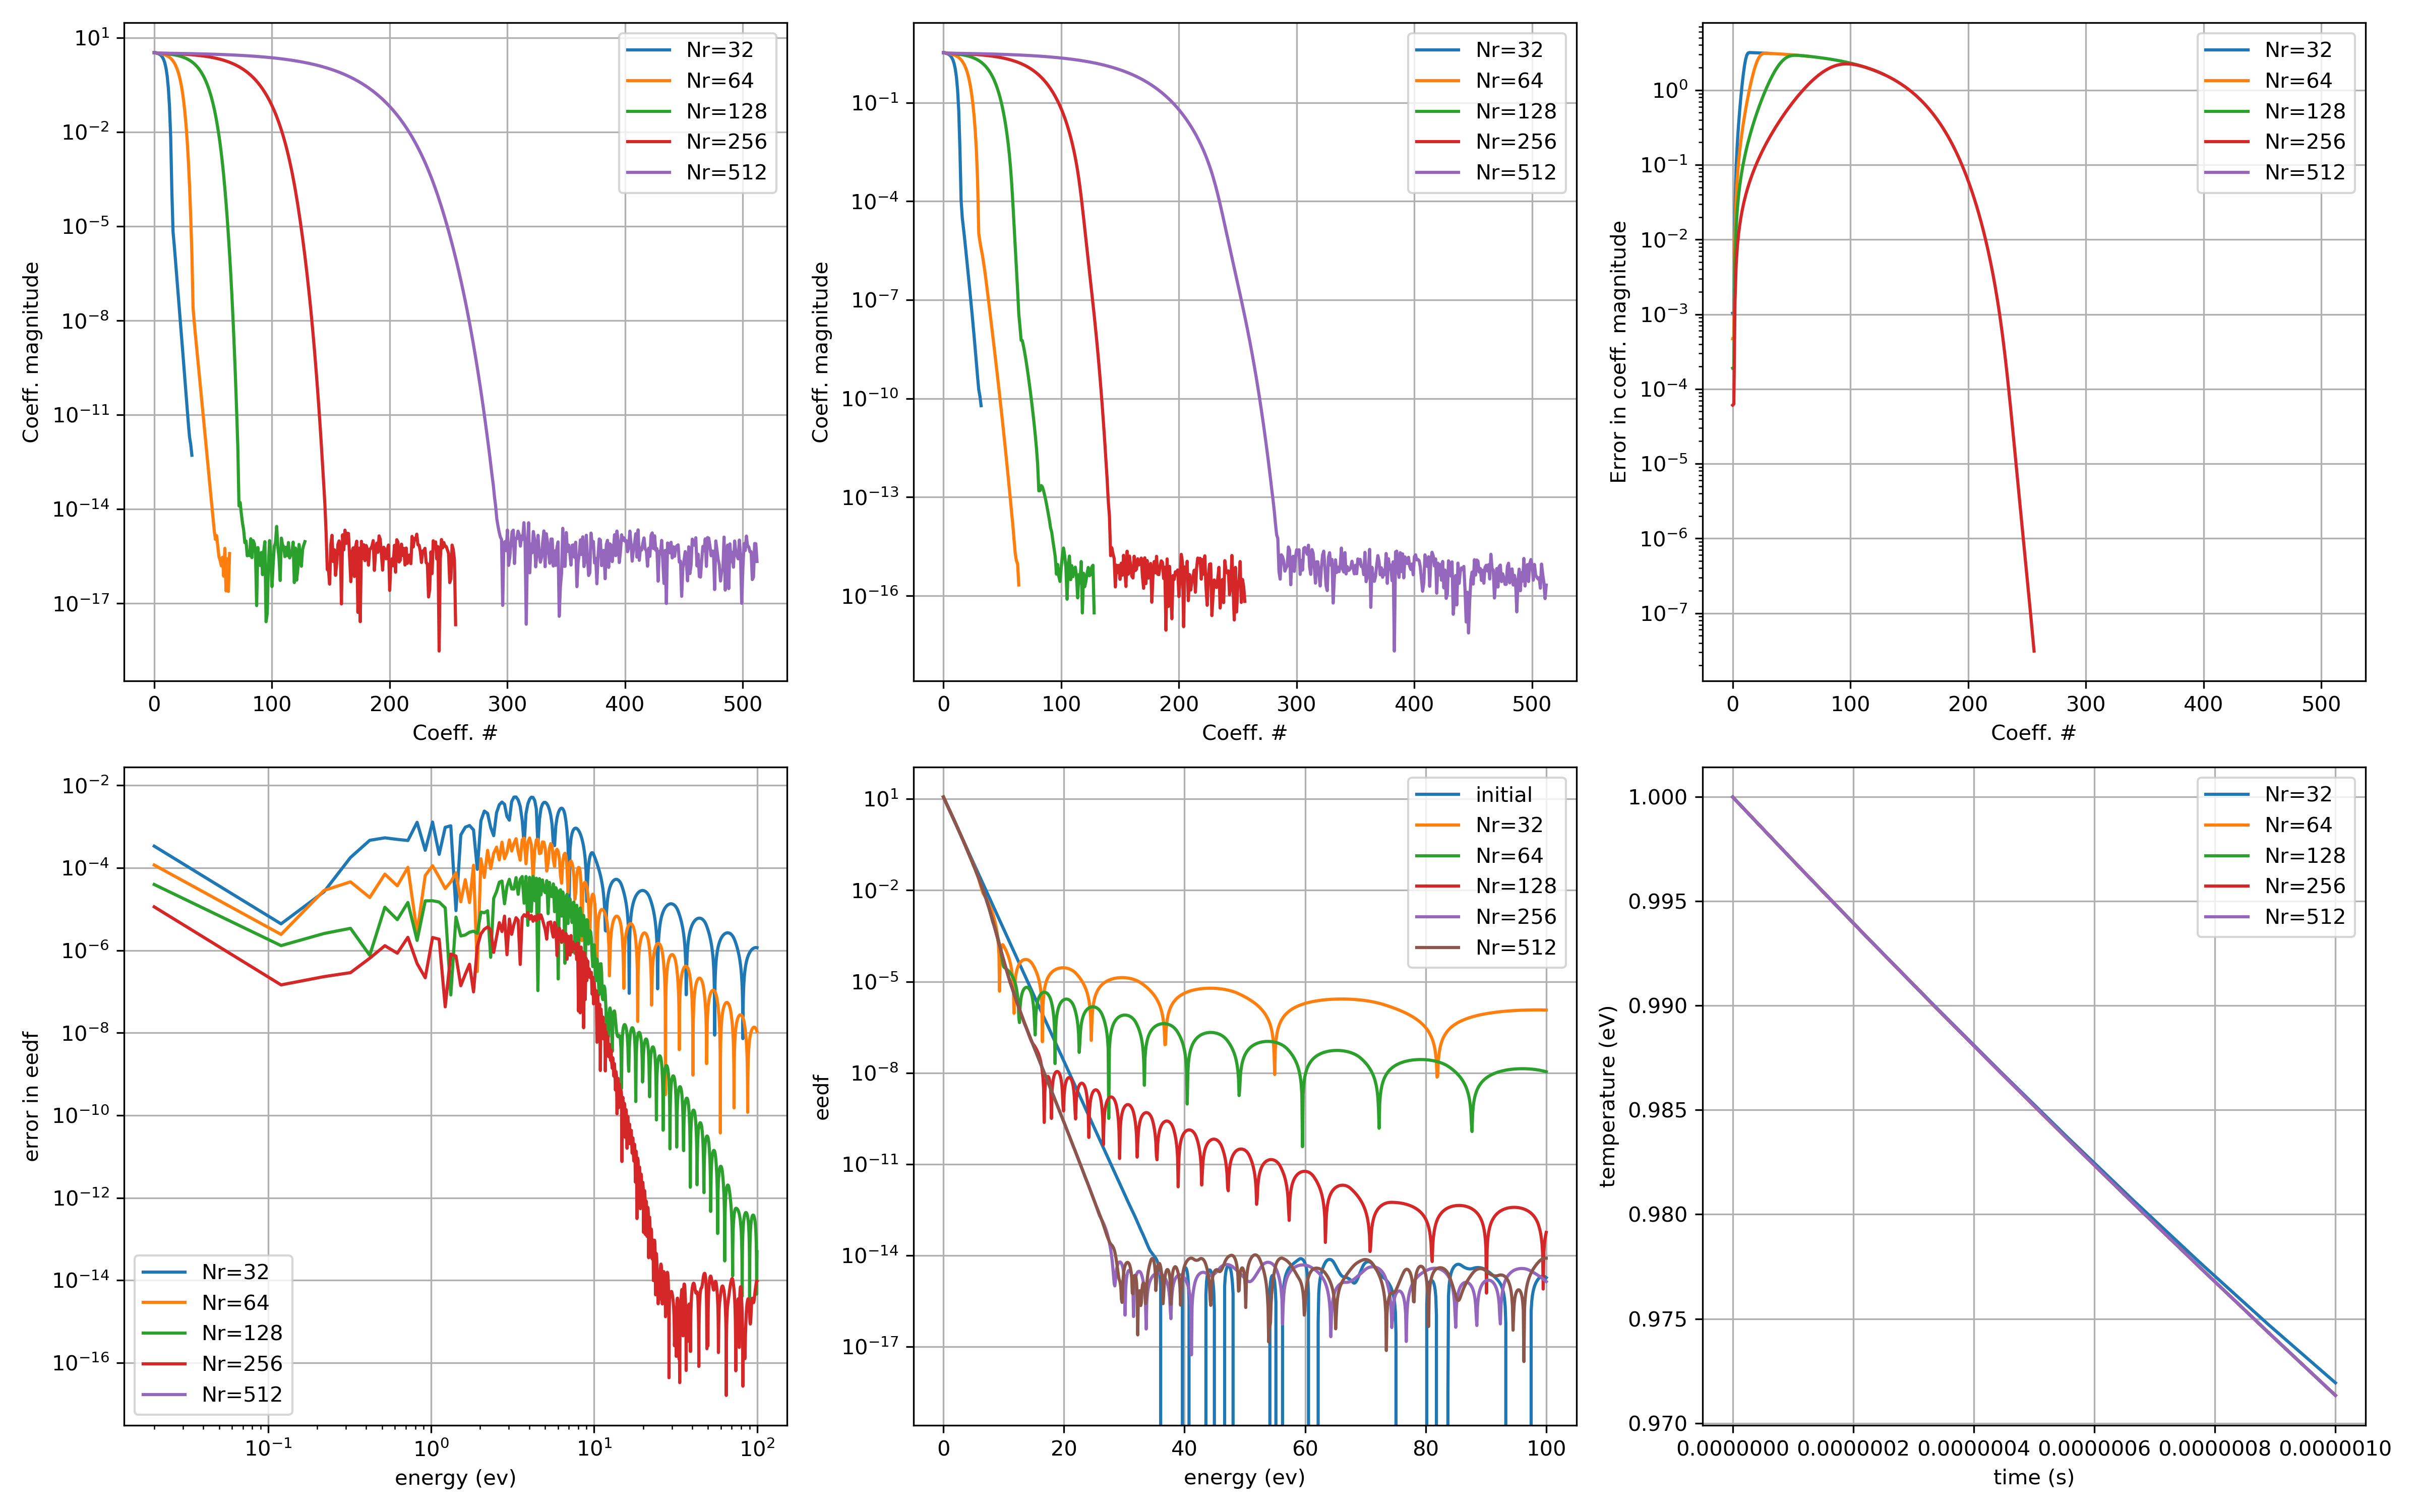
\includegraphics[width=0.6\textwidth]{figures/b_sp2_1ev_9.8e-1vth_coeff.png}
			\end{figure}
		}
		\only<+>{
			chosen $\beta = 0.96 \alpha$
			\begin{figure}
				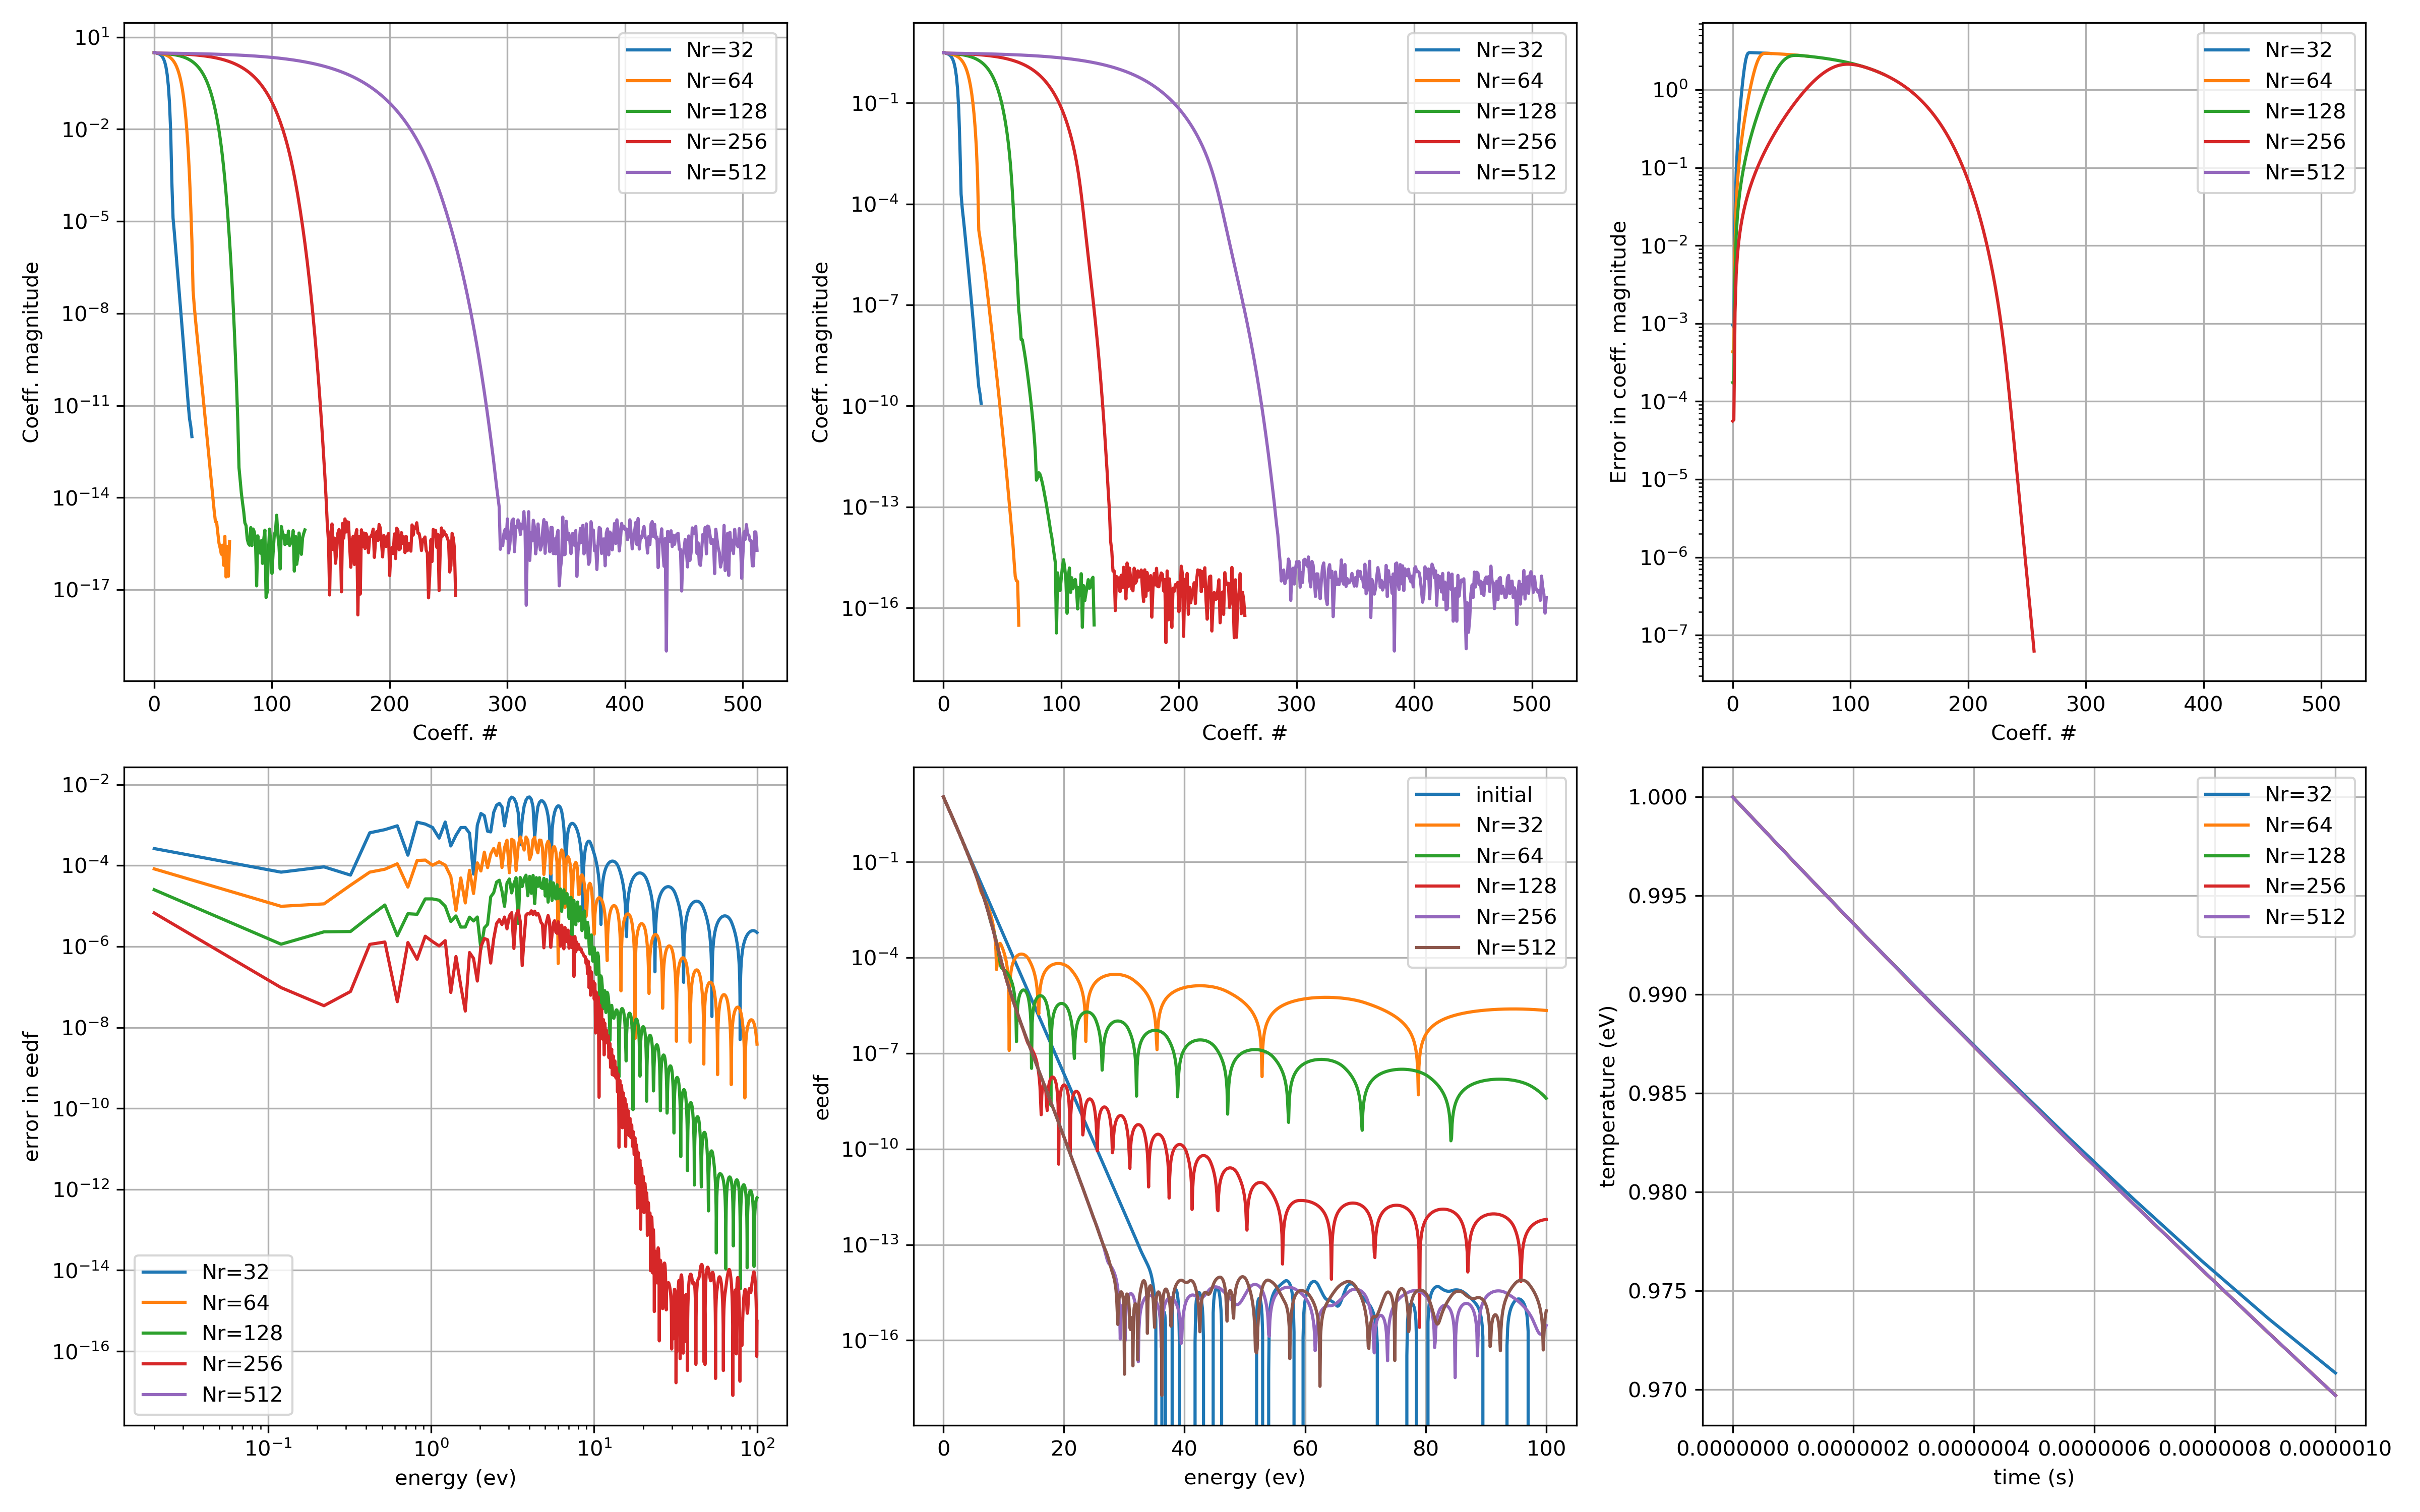
\includegraphics[width=0.6\textwidth]{figures/b_sp2_1ev_9.6e-1vth_coeff.png}
			\end{figure}
		}

		\only<+>{
			\begin{itemize}
				\item Log-spaced knot placement is not ideal for capturing tails. Struggles to capture the a perfect Maxwellian for energies > 40eV.
				\item Explore adaptive knot placement with appropriate error controls (i.e., binary tree with hierarchical splitting) ?
			\end{itemize}
		}
	
	\end{center}
\end{frame}





\begin{frame}
\frametitle{Convergence of expansion coefficients}
1eV, $\Delta t = 10^{-10}$ s, $t_{end} = 10^{-6}$ s\\
\includegraphics[width=0.99\textwidth]{figures/expansion_1ev.png}
\end{frame}

\begin{frame}
\frametitle{Convergence of expansion coefficients}
1eV, $\Delta t = 10^{-10}$ s, $t_{end} = 10^{-6}$ s\\
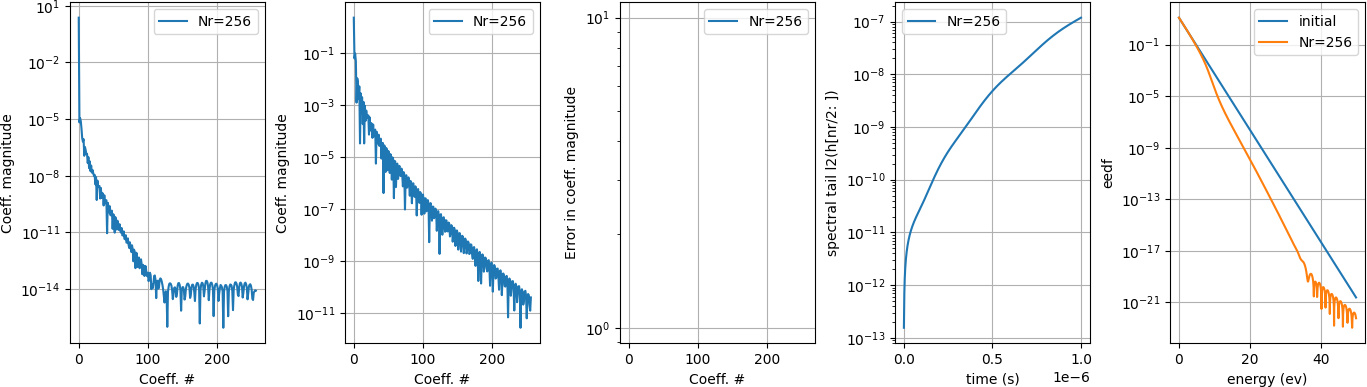
\includegraphics[width=0.99\textwidth]{figures/expansion_1ev_256.png}
\end{frame}

\begin{frame}
0.1ev\\
\includegraphics[width=0.99\textwidth]{figures/expansion_01ev.png}

5ev \\
\includegraphics[width=0.99\textwidth]{figures/expansion_5ev.png}
\end{frame}


\begin{frame}
\frametitle{V-space solver (with operator splitting)}
\begin{columns}
	\begin{column}{0.5\textwidth}
		\begin{center}
			\small
			\begin{align*}
			\partial_t f + \vect{E}\cdot \nabla_{\vect{v}} f = C[f]
			\end{align*}
			\begin{align*}
			&\left\{
			\begin{aligned}
			\partial_t f^{(0)} + \vect{E}\cdot \nabla_{\vect{v}} f^{(0)} &= 0, \quad t_n < t \leq t_n + \frac12 \Delta t \\
			f^{(0)}\of{t_n} &= f\of{t_n}
			\end{aligned}
			\right.
			\\
			&\left\{
			\begin{aligned}
			\partial_t f^{(1)} &= C[f^{(1)}], \quad t_n < t \leq t_n + \Delta t \\
			f^{(1)}\of{t_n} &= f^{(0)}\of{t_n + \frac12 \Delta t}
			\end{aligned}
			\right.
			\\
			&\left\{
			\begin{aligned}
			\partial_t f^{(2)} + \vect{E}\cdot \nabla_{\vect{v}} f^{(2)} &= 0, \quad t_n + \frac12 \Delta t < t \leq t_n + \Delta t  \\
			f^{(2)}\of{t_n} &= f^{(1)}\of{t_n + \Delta t}
			\end{aligned}
			\right.
			\\
			& f\of{t_n + \Delta t} = f^{(2)}\of{t_n + \Delta t}
			\end{align*}
		\end{center}
	\end{column}
	\begin{column}{0.5\textwidth}  %%<--- here
		\begin{center}
			Overall algorithm: given $\vect{v}_0$, $a_{klm}$ at $t_n$:
			\begin{enumerate}
				\item $\vect{v}_0 \leftarrow \vect{v}_0 - \myint_{t_n}^{t_n+\frac12 \Delta t} \vect{E}\of{\tau} d\tau$
				\item Solve collision op.  from $t_0$ to $t_0 + \Delta t$
				\item $\vect{v}_0 \leftarrow \vect{v}_0 - \myint_{t_n+\frac12 \Delta t}^{t_n + \Delta t} \vect{E}\of{\tau} d\tau$
			\end{enumerate}
		\end{center}
	\end{column}
\end{columns}
\end{frame}

\begin{frame}
	\frametitle{EEDF : Maxwell Polynomials (T=1e-6 s)}
	\begin{center}
		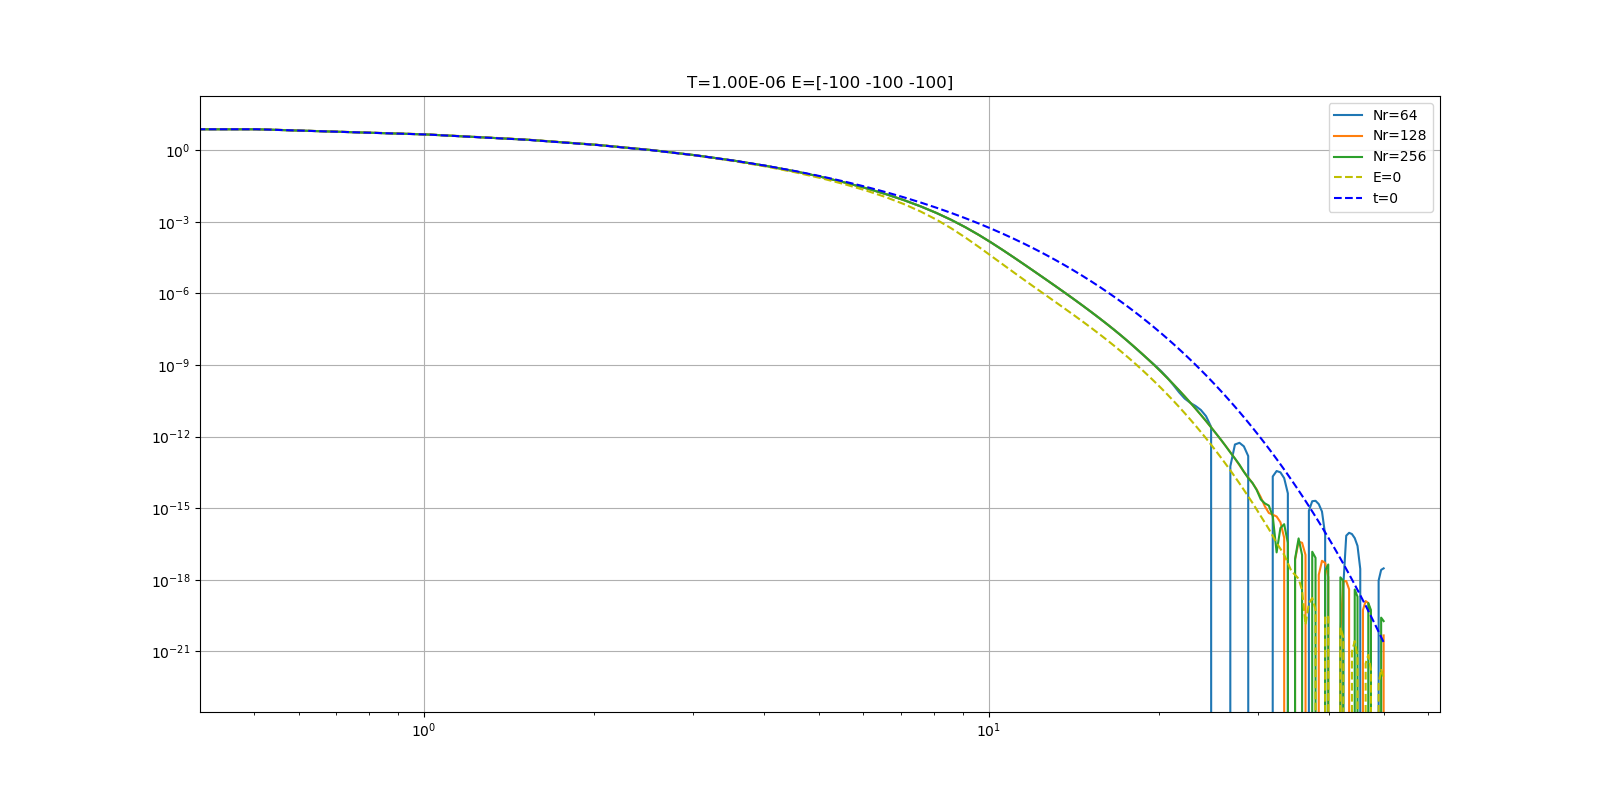
\includegraphics[width=0.9\textwidth]{figures/g0_1_maxwell_eedf.png}
	\end{center}
\end{frame}

\begin{frame}
	\frametitle{EEDF : Maxwell Polynomials (T=1e-6 s)}
	\begin{center}
		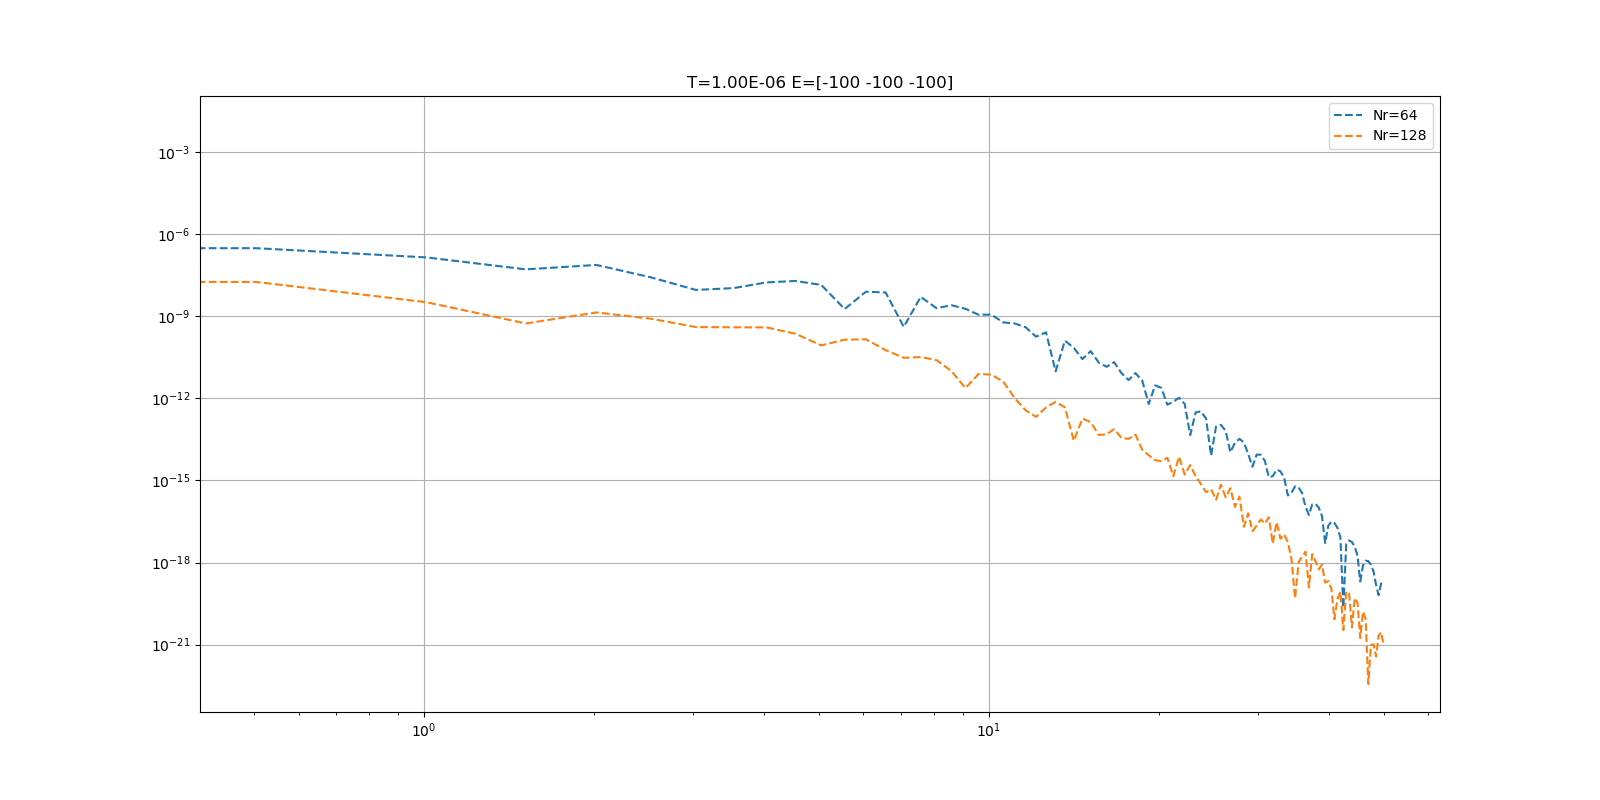
\includegraphics[width=0.9\textwidth]{figures/g0_1_maxwell_eedf_conv.png}
	\end{center}
\end{frame}

\begin{frame}
	\frametitle{EEDF : linear b-splines (T=1e-6 s)}
	\begin{center}
		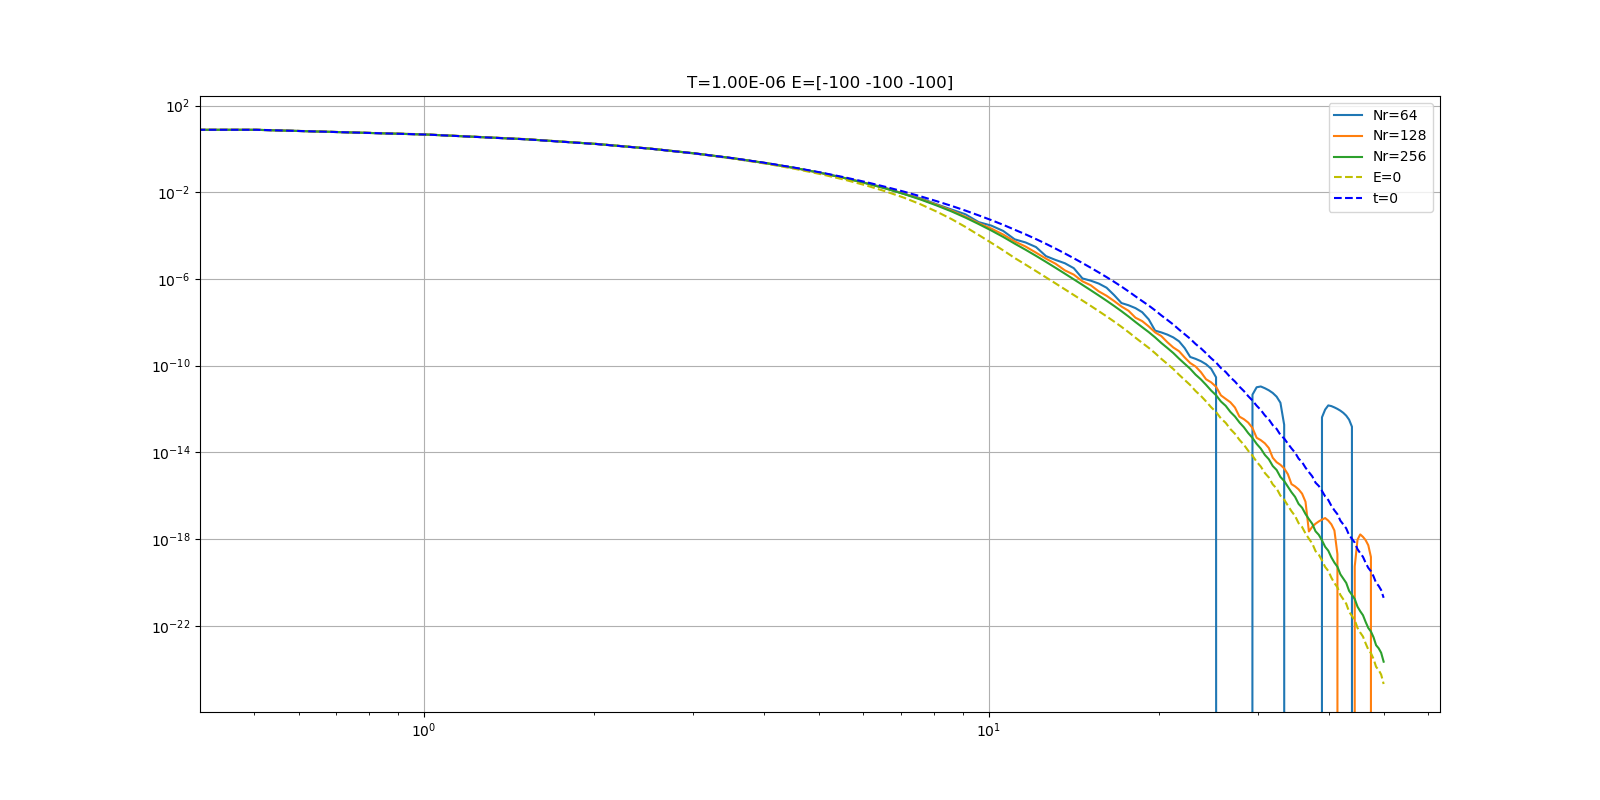
\includegraphics[width=0.9\textwidth]{figures/g0_1_bspline_eedf.png}
	\end{center}
\end{frame}

\begin{frame}
	\frametitle{EEDF : linear b-splines (T=1e-6 s)}
	\begin{center}
		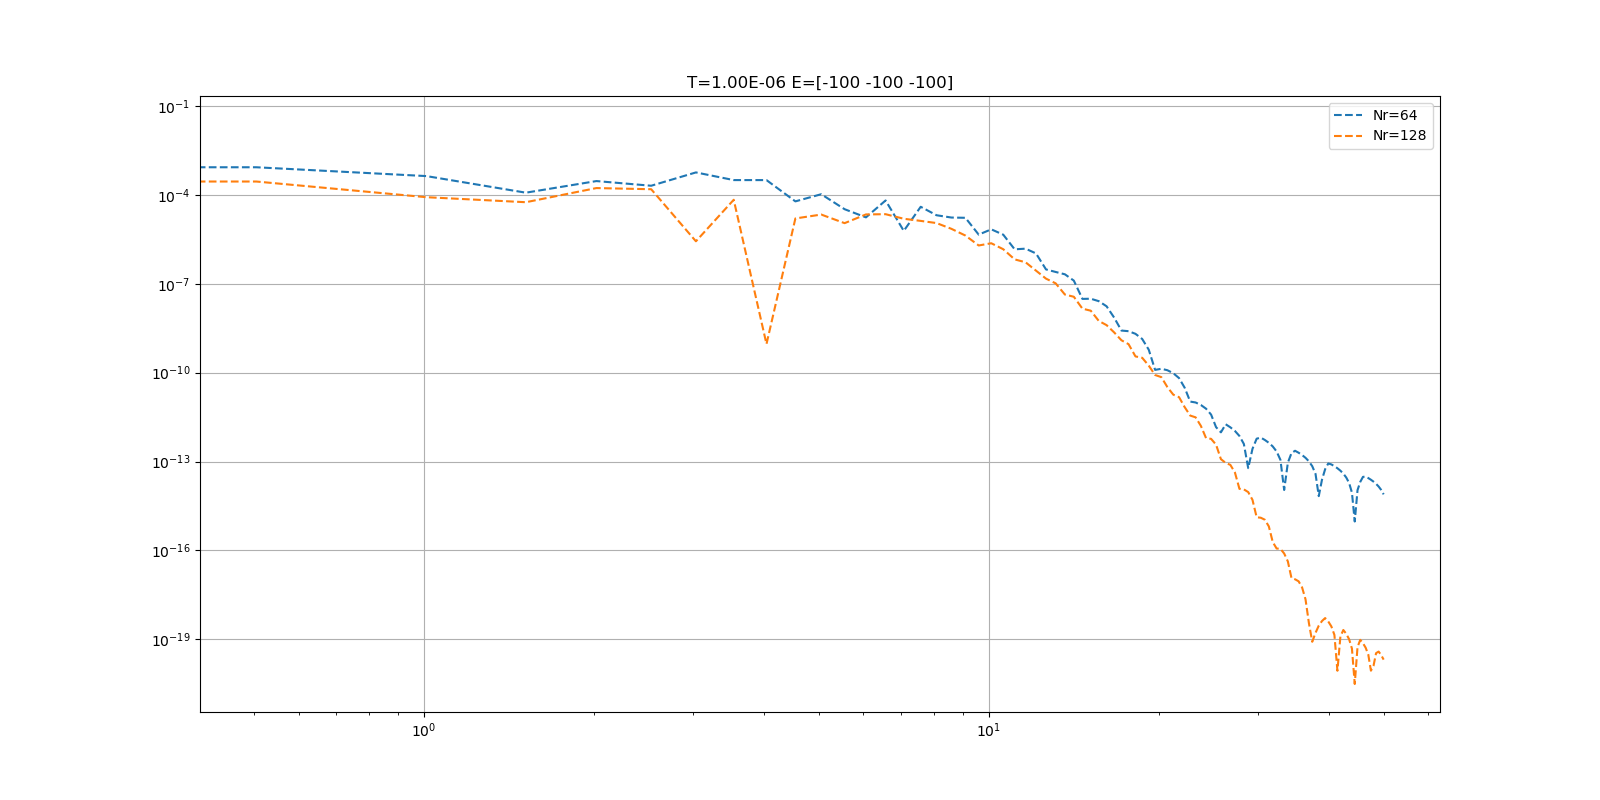
\includegraphics[width=0.9\textwidth]{figures/g0_1_bspline_eedf_conv.png}
	\end{center}
\end{frame}



\begin{frame}
	\frametitle{EEDF : Maxwell Polynomials (T=3e-6 s)}
	\begin{center}
		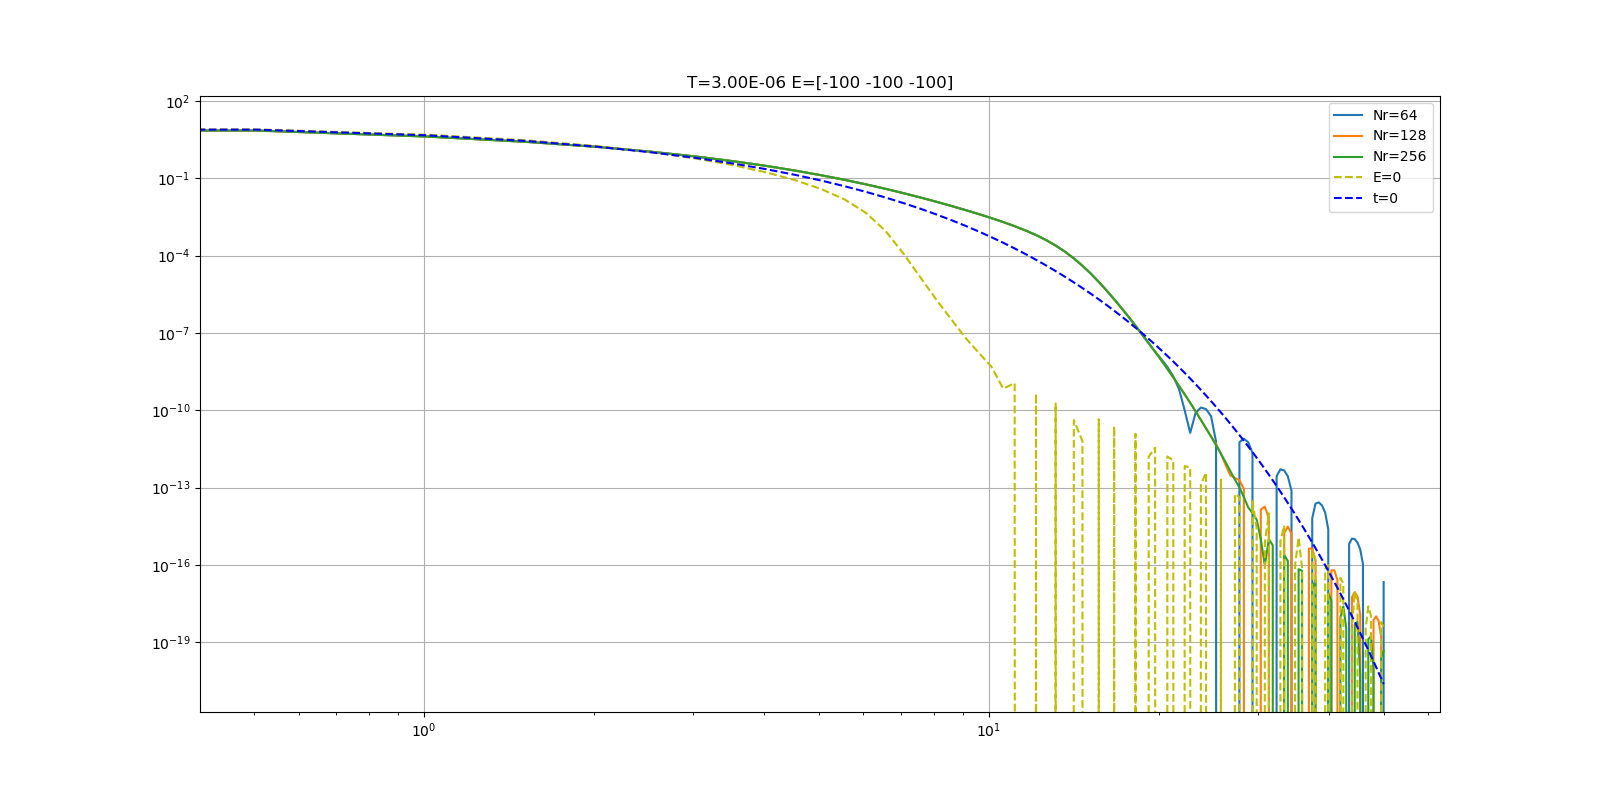
\includegraphics[width=0.9\textwidth]{figures/g0_3_maxwell_eedf.png}
	\end{center}
\end{frame}

\begin{frame}
	\frametitle{EEDF : Maxwell Polynomials (T=3e-6 s)}
	\begin{center}
		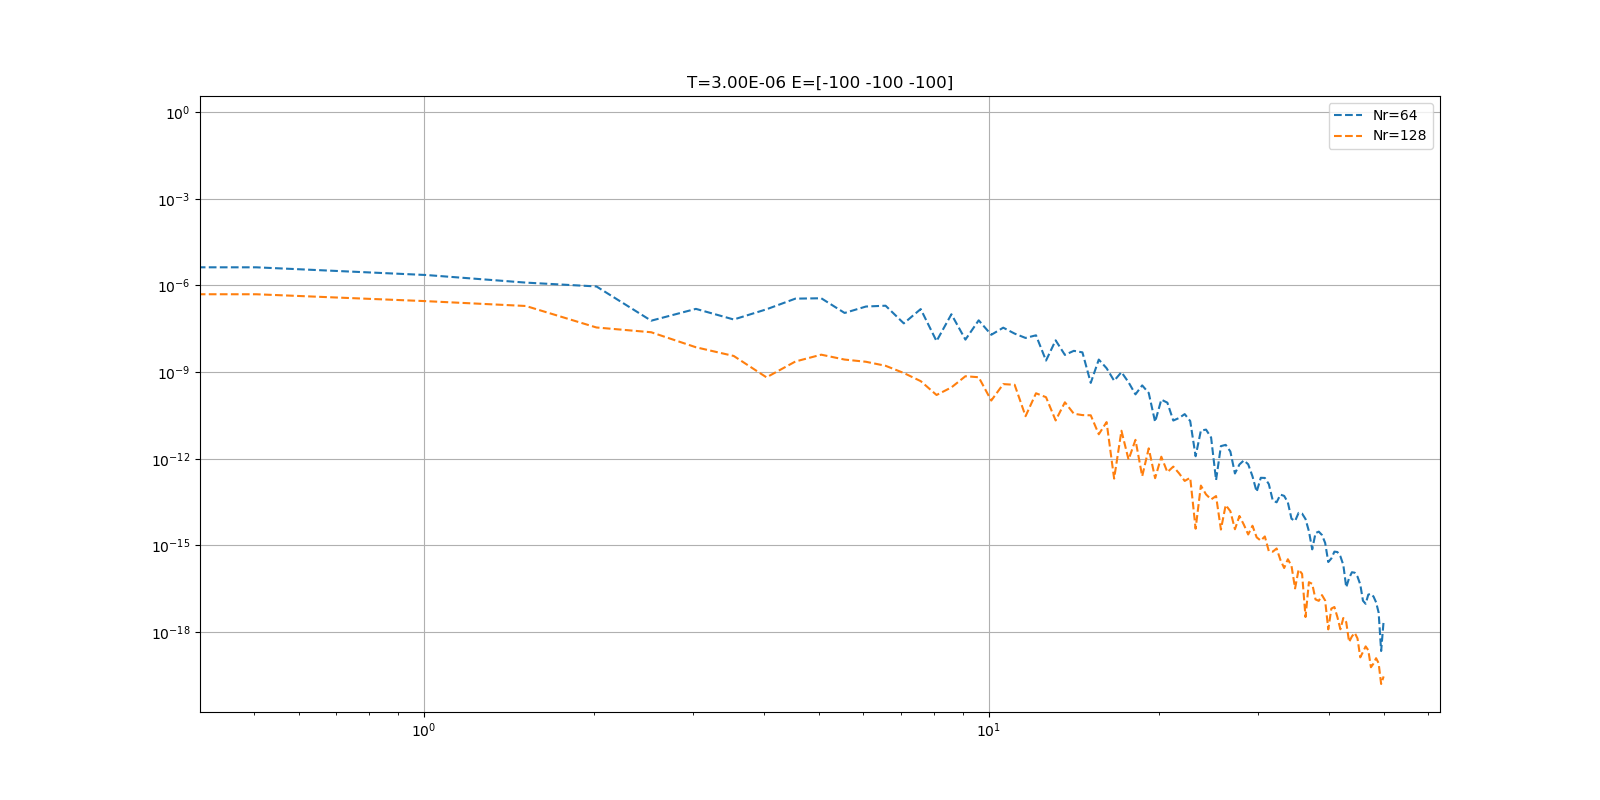
\includegraphics[width=0.9\textwidth]{figures/g0_3_maxwell_eedf_conv.png}
	\end{center}
\end{frame}

\begin{frame}
	\frametitle{EEDF : linear b-splines (T=3e-6 s)}
	\begin{center}
		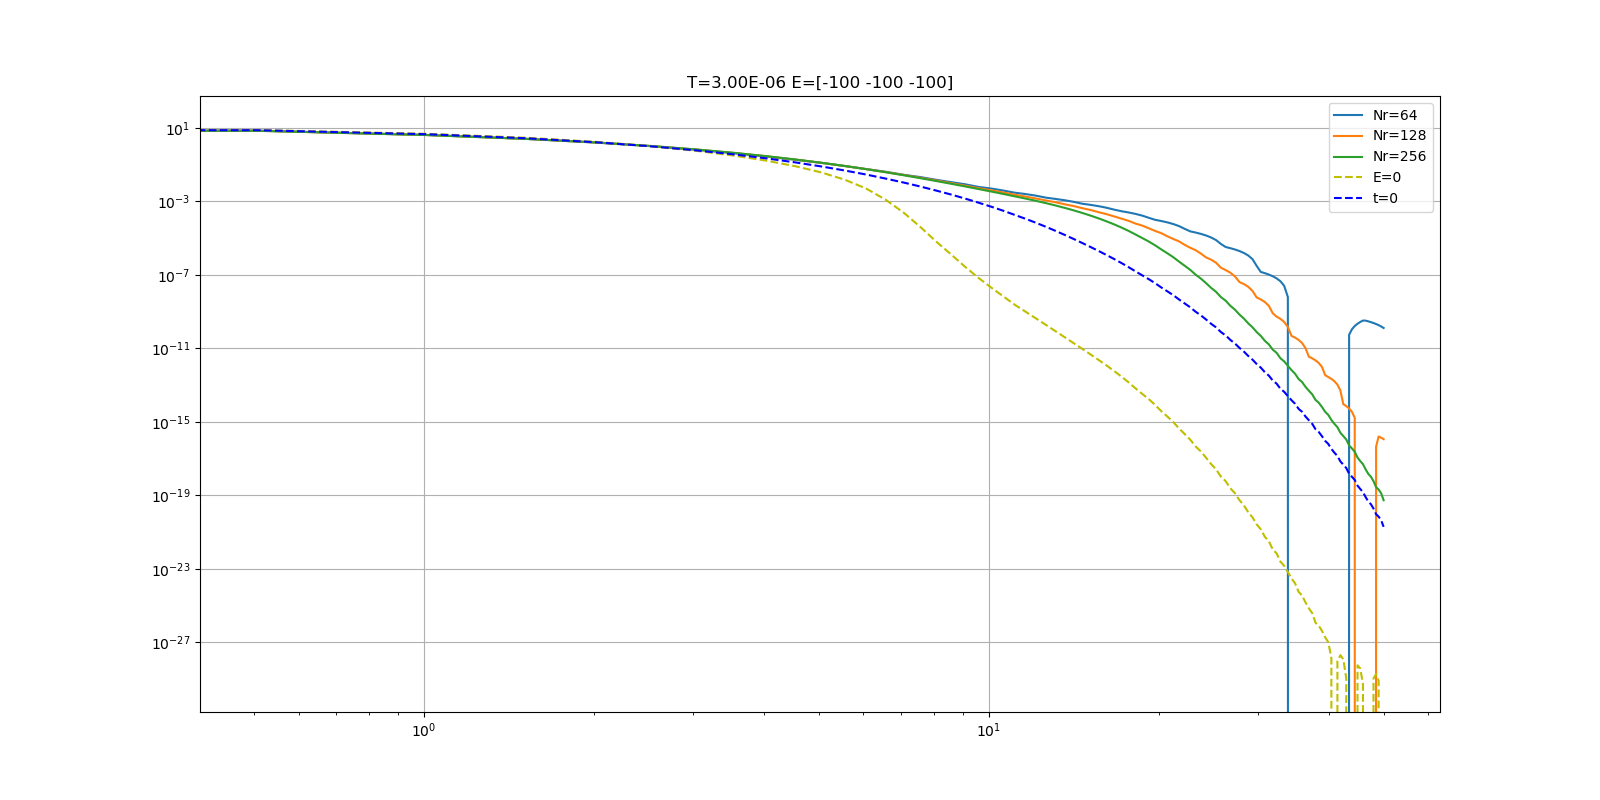
\includegraphics[width=0.9\textwidth]{figures/g0_3_bspline_eedf.png}
	\end{center}
\end{frame}

\begin{frame}
	\frametitle{EEDF : linear b-splines (T=3e-6 s)}
	\begin{center}
		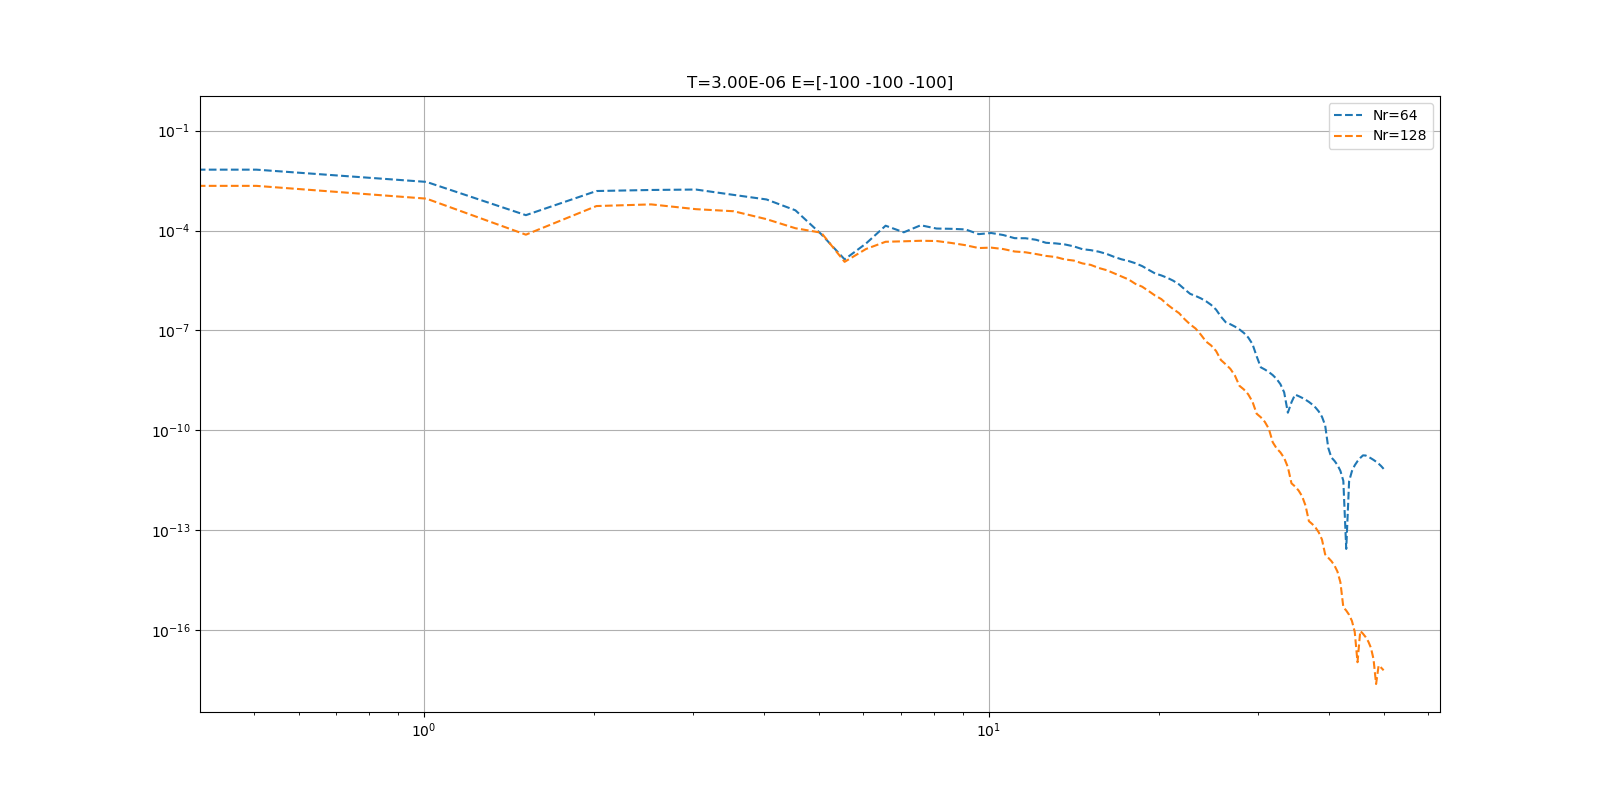
\includegraphics[width=0.9\textwidth]{figures/g0_3_bspline_eedf_conv.png}
	\end{center}
\end{frame}


\begin{frame}
	\frametitle{EEDF : Maxwell vs. b-splines}
	\begin{center}
		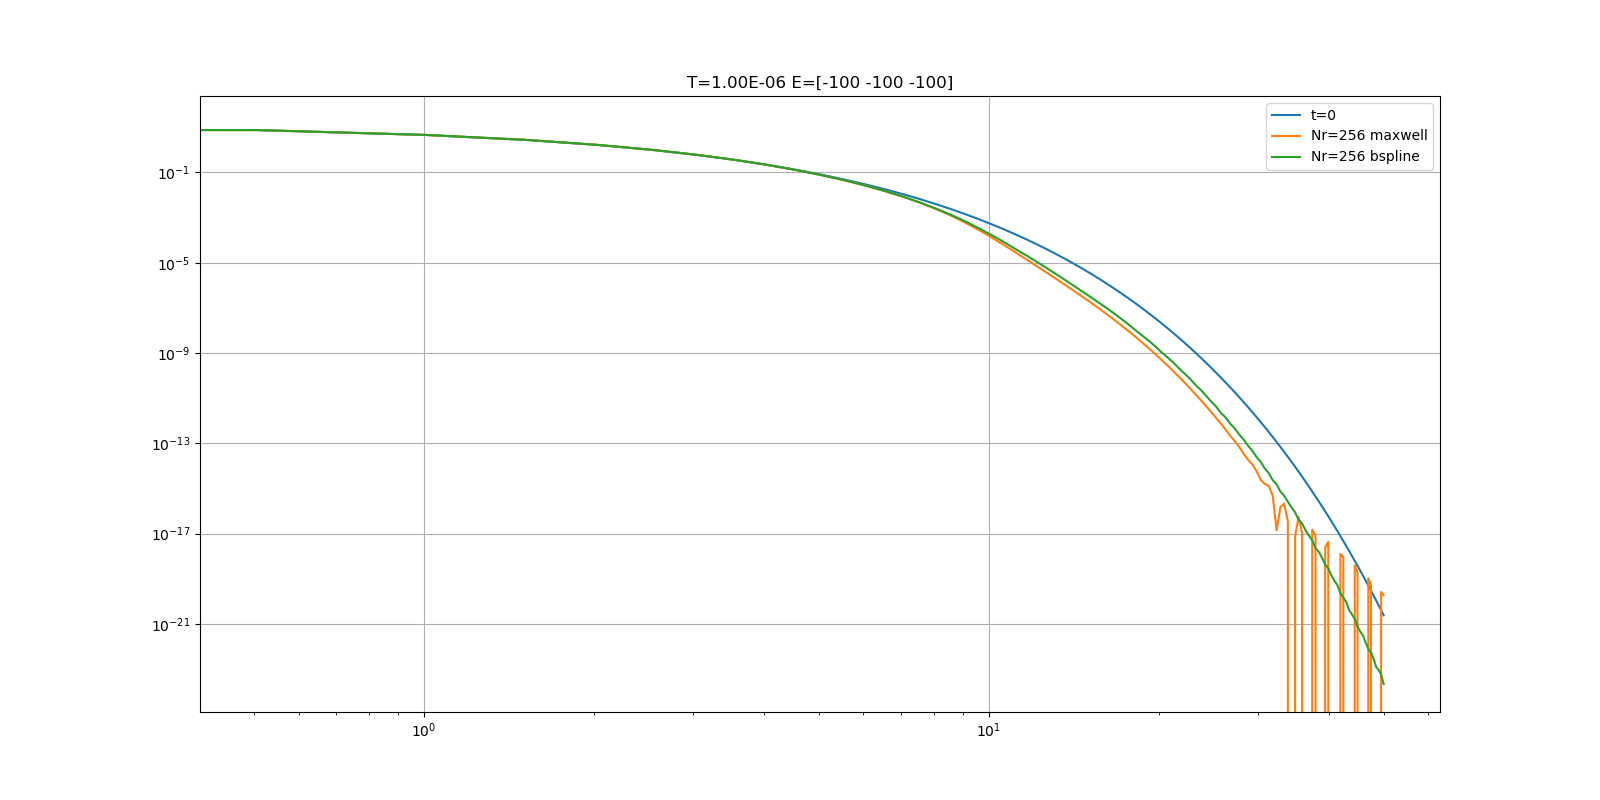
\includegraphics[width=0.9\textwidth]{figures/g0_1_bspline_vs_maxwell.png}
	\end{center}
\end{frame}

\begin{frame}
	\frametitle{EEDF : Maxwell vs. b-splines}
	\begin{center}
		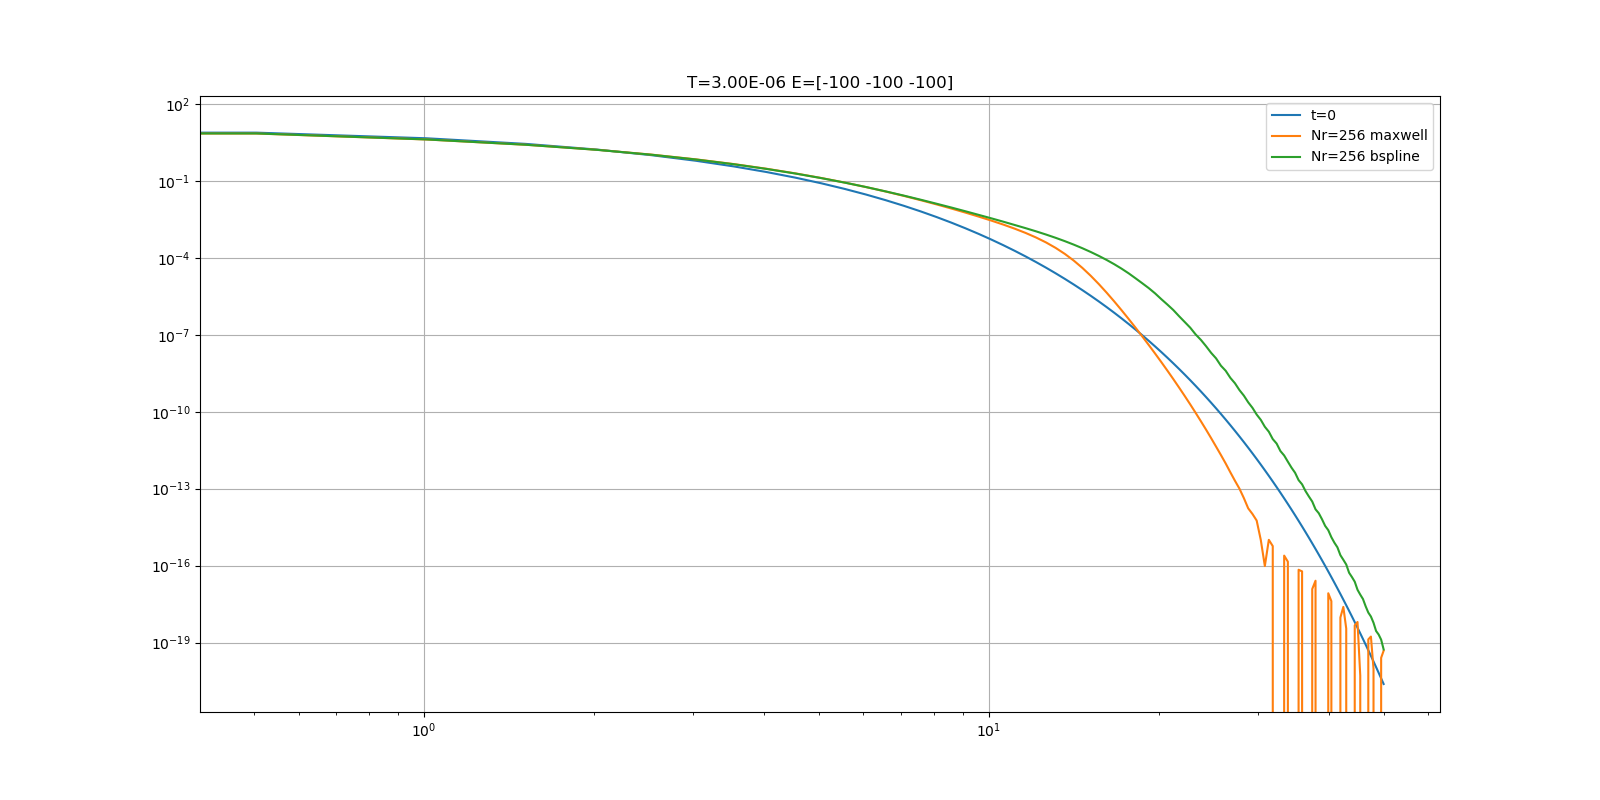
\includegraphics[width=0.9\textwidth]{figures/g0_3_bspline_vs_maxwell.png}
	\end{center}
\end{frame}





%===============================================================================
\end{document}

